\documentclass[11pt]{article}
\pdftrailerid{}
\pdfsuppressptexinfo=15
\usepackage[T1]{fontenc}
\usepackage{lmodern}
\usepackage[margin=1in]{geometry}
\usepackage{amsmath,amssymb,amsthm,mathtools}
\usepackage{microtype}
\usepackage{enumitem}
\usepackage{booktabs,array,longtable}
\usepackage{xcolor}
\usepackage{graphicx}
\usepackage{tikz}
\usetikzlibrary{arrows.meta,positioning,calc,decorations.pathreplacing,shapes.geometric,fit,backgrounds,matrix}
\usepackage[numbers,sort&compress]{natbib}
\usepackage{url}
\usepackage{hyperref}
\hypersetup{colorlinks=true,linkcolor=blue!45!black,citecolor=green!35!black,urlcolor=blue!50!black,
  pdftitle={Almost-Linear-Time Maximum-Cardinality Matching in General Graphs},pdfauthor={OpenAI},
  pdfsubject={Uniform exact maximum matching and prescribed-degree factor search with every-path almost-linear input-size running time}}
\urlstyle{same}
\numberwithin{equation}{section}
\newtheorem{theorem}{Theorem}[section]
\newtheorem{lemma}[theorem]{Lemma}
\newtheorem{proposition}[theorem]{Proposition}
\newtheorem{corollary}[theorem]{Corollary}
\theoremstyle{definition}
\newtheorem{definition}[theorem]{Definition}
\theoremstyle{remark}
\newtheorem{remark}[theorem]{Remark}
\DeclareMathOperator{\OPT}{OPT}
\DeclareMathOperator{\PM}{PM}
\DeclareMathOperator{\polylog}{polylog}
\DeclareMathOperator{\supp}{supp}
\DeclareMathOperator{\rank}{rank}
\DeclareMathOperator{\TV}{TV}
\DeclareMathOperator{\dist}{dist}
\DeclareMathOperator{\vol}{vol}
\newcommand{\E}{\mathbb E}
\setlist{topsep=4pt,itemsep=3pt,parsep=0pt}
\setlength{\emergencystretch}{1.5em}
\setcounter{tocdepth}{2}
\allowdisplaybreaks[2]

\title{Almost-Linear-Time Maximum-Cardinality\\Matching in General Graphs}
\author{OpenAI}
\date{September 24, 2026}
\begin{document}
\maketitle
\begin{abstract}
We prove that maximum-cardinality matching in a simple undirected graph with
$n$ vertices and $m$ edges can be found by one uniform randomized algorithm in
$(n+m)^{1+o(1)}$ time. The bound holds on every computation path in a
logarithmic-word model, and the algorithm returns an explicit maximum matching
with probability at least $2/3$.
An explicit reduction gives the same time and probability guarantees for
deciding whether a simple host graph has a spanning subgraph with prescribed
valid vertex degrees, and for finding one when it exists.
\end{abstract}
\tableofcontents
\clearpage
\section{Introduction}\label{sec:introduction}

A matching in a graph is a set of edges with pairwise disjoint endpoints.
The maximum-cardinality matching problem asks for such a set with the largest
possible number of edges. We prove an almost-linear bound in the adjacency-list
input size for general graphs, with explicit output and a single uniform algorithm.
The running-time guarantee includes every unsuccessful random computation,
all finite-precision work, and all input and output costs.

\subsection{Statement and computational model}

The input is a simple undirected unweighted graph $G=([n],E)$, where $n\ge1$
and $m=|E|$. It is given by an array of adjacency-list boundaries and two
neighbor occurrences per edge. Labels and indices use $O(\log(n+2))$ bits.
The lists may have any valid order. Isolated vertices count toward $n$, and
the graph need not be connected. Write $p=n+m$, which is within a constant
factor of the number of input word records, and write $\nu(G)$ for the maximum
matching size.

We use a classical randomized word-RAM whose word length is
\[
                     w=\lceil c_0\log_2(n+2)\rceil,
\]
for a fixed constant $c_0\ge2$ chosen with the algorithm. Unit-cost instructions
are word reads and writes, comparison, addition, subtraction, multiplication
modulo $2^w$, integer quotient and remainder with nonzero divisor, Boolean
operations, and shifts by fewer than $w$ positions. Each independent fair
random bit costs one instruction. Longer arithmetic uses charged multiword
implementations. Allocation, initialization, data movement, preprocessing,
and output writing are included. There is no oracle or nonuniform advice.
Since $n\le p\le n^2$ for a simple graph, the word length is also
$\Theta(\log(p+2))$.

\begin{theorem}[Exact matching in almost-linear input-size time]\label{thm:main}
There are a single uniform randomized word-RAM algorithm, fixed constants
$c_0\ge2$ and $C\ge1$, and a nonincreasing function
$\eta:\mathbb N_{\ge1}\to\mathbb R_{\ge0}$ with $\eta(q)\to0$ as
$q\to\infty$ such that the following holds.
For every input graph $G=([n],E)$ with $m=|E|$ and $p=n+m$, the algorithm
halts on every computation path in at most
\[
                          C p^{1+\eta(p)}
\]
instructions. With probability at least $2/3$ it outputs an explicit list of
edges of a matching of size $\nu(G)$.
\end{theorem}

For every fixed integer $\kappa\ge1$, this gives
$C_\kappa n^{1+\eta(n)}$ instructions on graphs with $m\le\kappa n$, for
some constant $C_\kappa$. The same algorithm and exponent envelope work for
all $\kappa$, which need not be supplied as an input. At the dense extreme
$m=\Theta(n^2)$, the bound is $n^{2+o(1)}$.

A perfect matching is not promised. In particular, the perfect-matching
procedure for graphs of maximum degree three will be used only after
reductions that preserve explicit witnesses. A separate algorithm for each fixed exponent slack
would also be insufficient; Section~\ref{sec:uniformization} constructs the
single finite program and the common envelope in Theorem~\ref{thm:main}.

A reduction also gives an almost-linear bound for prescribed vertex degrees. Given an
integer $f(v)$ with $0\le f(v)\le\deg_G(v)$ for every vertex $v$, an
\emph{$f$-factor} is a spanning subgraph $([n],F)$ with
$\deg_F(v)=f(v)$ for every $v$. Corollary~\ref{cor:f-factor} gives one
uniform randomized algorithm that decides whether an $f$-factor exists and
returns its edge list when it does, with success probability at least $2/3$
and $(n+m)^{1+o(1)}$ instructions on every computation path. The degree
prescription is an array of one-word integers. Section~\ref{sec:f-factors}
gives the witness-preserving reduction with only logarithmic expansion in
the number of edge incidences.

\subsection{Context and significance}

The structure of matchings has long connected combinatorial existence
criteria with efficient construction. Hall's theorem characterizes when
a family of sets has distinct representatives~\cite{Hall1935}, and Tutte's
perfect-matching theorem identifies the obstruction caused by odd
components~\cite{Tutte1947}. Berge's augmenting-path criterion turns
maximum cardinality into a question about alternating
paths~\cite{Berge1957}. Edmonds made this approach algorithmic in general
graphs through blossom contraction and expansion~\cite{EdmondsPaths}.
His matching-polytope theorem gives a complementary explanation of the
odd-set constraints~\cite{EdmondsPolytope}: vertex-degree inequalities
alone allow, for example, value $1/2$ on each edge of a triangle.

Tutte's short proof of the factor theorem reduces prescribed-degree
$f$-factors to perfect matchings~\cite{Tutte1954Factor}. The reduction in
Section~\ref{sec:f-factors} follows this incidence-port approach, replacing
the local complete connections to auxiliary vertices by the rearrangeable
networks used in Section~\ref{sec:uniformization}. This controls the size of
the perfect-matching instance even when a host vertex has high degree.
There are also direct algorithms: Gabow finds a maximum-cardinality edge
set subject to $\deg_F(v)\le f(v)$ in $O(n^{2/3}m)$ time on simple
graphs~\cite[Theorem~4.1]{Gabow2025FMatching}. After linear-time input
processing, including removal of zero-demand vertices, this gives an
$O(n+n^{2/3}m)$ factor test: an $f$-factor exists exactly when the returned
set has $2|F|=\sum_v f(v)$.

Batching shortest augmenting paths led to the bipartite algorithms of
Hopcroft and Karp~\cite{HopcroftKarp1973} and, independently,
Karzanov~\cite{Karzanov1973Representatives}, and to the Micali--Vazirani
algorithm for general graphs~\cite{MicaliVazirani,MicaliVaziraniAnalysis}.
The latter has running time $O(m\sqrt n)$ on a RAM; reading the explicit
input and removing isolates gives the convenient universal bound
$O(n+m\sqrt n)$. This is $O_\kappa(n^{3/2})$ when $m\le\kappa n$.
Gabow and Tarjan developed a different route through weighted
scaling~\cite{GabowTarjan1991}, and Gabow later gave a direct
weighted-search formulation at the same cardinality bound~\cite{Gabow2017}.
On very dense graphs, Goldberg and Karzanov improve the combinatorial bound to
$O(n+m\sqrt n\log(n^2/m)/\log n)$ by combining skew-symmetric flow
with graph compression~\cite[Theorem~10.3]{GoldbergKarzanov2004}.
The weighted problem has its own sequence of improvements: the scaling
algorithm of Duan, Pettie, and Su finds an exact maximum-weight matching in
$O(m\sqrt n\log(nW))$ time for integer weights of magnitude at most
$W$~\cite{DuanPettieSu2018}, with logarithms bounded below by a constant.

Algebraic methods offer another important approach. Random evaluation
of the Tutte matrix connects matching to linear algebra~\cite{Lovasz1979}.
Mucha and Sankowski, and subsequently Harvey, obtained randomized
algorithms that construct maximum matchings at the matrix-multiplication
time scale, conventionally written $O(n^\omega)$
field operations~\cite{MuchaSankowski2004,Harvey2009}.
These algorithms already recover explicit witnesses and can work over
finite fields of polynomial size. Their matrix-multiplication bound is
most competitive on dense graphs. Theorem~\ref{thm:main} instead gives an
almost-linear bound in the explicit input size throughout the range of
densities, including $n^{2+o(1)}$ at the dense extreme.

For bipartite matching, the unit-capacity flow formulation permits
continuous optimization to accelerate exact search. M\k{a}dry's
electrical-flow interior-point method~\cite{Madry2013CentralPath} and
the moderately dense algorithm of van den Brand
et al.~\cite{vanDenBrandEtAl2020BipartiteMatching} were intermediate
advances. The almost-linear exact integral-flow algorithms of Chen
et al.~\cite{FlowRandomized} and van den Brand
et al.~\cite{FlowDeterministic} then yield almost-linear exact bipartite
matching. General graphs require additional control of odd blocks.
Here that control is provided by the matching state and its local
projections. The deterministic flow theorem is used through the
explicit static interface in Lemma~\ref{lem:integral-flow}.

The proof combines several established ideas with interfaces tailored
to that state. Its constructive factor-critical blocks belong to the
contraction-and-expansion tradition, while Hall's theorem underlies
the reassignment of their exposed vertices. The multiscale allocation
and debt bounds are proved directly. The routing helper uses the
cut-matching structure of Khandekar, Rao, and
Vazirani~\cite{KhandekarRaoVazirani2006}, together with concentration
and conductance estimates~\cite{TroppBernstein,SinclairJerrum1989}.
Its recursive virtual graphs follow the hierarchical random-walk
embeddings of Ghaffari, Kuhn, and Su~\cite[Section~3.1.2]{GhaffariKuhnSu2017}.
Here the sampled support and the substituted routes must also preserve
supplied resource loads, with their full construction costs charged.

The use of approximate minimum-ratio circulations as optimization
directions has its modern antecedent in the almost-linear flow
framework~\cite{FlowRandomized,FlowDeterministic}. Chen et al.
prove a deterministic \emph{fully dynamic} approximate
minimum-ratio-cycle theorem with flat forest
representations~\cite[Definition~2.3 and Theorem~3.5]{IncrementalGraphs}.
Our routing hierarchy is related to the origin-aware construction of
Rozho\v{n} et al.~\cite{MinorAggregateRouting}; the finite forest family
and associated cycle extraction adapt the construction in
\cite[Section~4.5]{IncrementalGraphs}. The preallocated forest copies used
to lift recursive paths follow Kyng, Meierhans, and Probst
Gutenberg~\cite[Section~3.3, Lemma~3.21 and Algorithm~5]{KyngMeierhansProbstGutenberg2023FlatForest}.
Sections~\ref{sec:engine} and~\ref{sec:backend-updates} specify how retained
mapped edges preserve accumulated coordinate changes and absolute motion
through these representation updates. The recent distance-oracle
approach of Kyng et al.~\cite{MinRatioDistanceOracles2026} provides
another development of this method. Sections~\ref{sec:backend-quality}
and~\ref{sec:backend-updates} supply the complete backend used here,
including its adaptive guarantees, explicit changes of representation,
stable edge-copy lifetimes, and bounds on traversal length before
cancellation. Those guarantees are the inputs to our priced-step
analysis.

\subsection{Main ideas and organization}

The central subproblem is to find a perfect matching in a graph of maximum
degree three.  Section~\ref{sec:uniformization} reduces exact cardinality
queries to this subproblem while retaining the original edge identifiers,
so that every successful answer can be decoded into a matching of the
input graph.

The perfect-matching procedure maintains a current matching through a
partition of the vertices.  Its odd blocks, called \emph{bins}, come with
internal matchings after any prescribed vertex is left exposed.
Some outside singleton vertices, called \emph{rows}, are assigned along
original edges to distinct bins.  Each assigned bin matches its exposed
vertex to its row; an unassigned bin contributes one unmatched vertex.
The remaining vertices are stored as matched pairs, apart from unmatched
vertices set aside during repairs.  This representation permits a change
of exposure without immediately expanding a nested block.

The difficulty is to repair this representation after structural changes
without repeatedly scanning all its odd blocks. A \emph{ledger} allocates
a fixed amount from each row among its neighboring bins. The difference
between a bin's capacity and its allocated load is its residual. Several
ledgers impose residual margins proportional to bin size; a nonnegative
\emph{debt} allows a margin to fail temporarily. At each settled state,
the lowest ledger has no debt and certifies a strict Hall surplus for
every nonempty set of bins. The highest ledger carries a logarithmic
objective that must admit progress when a perfect matching exists and no
structural operation is available.

The intermediate ledgers turn that progress into affordable repairs. A
repair is an exact flow problem on row--bin incidences, initially explored
only at bins whose debt is substantial relative to their size. An
unexplored boundary bin temporarily accepts an optimistic amount of flow.
If enough arrives, the algorithm explores that bin and permanently locks
in an absorbed amount proportional to its size. The total available flow
is bounded by the starting debt, so these locks bound the number of
physical vertices examined. If the requested residual margin is
infeasible, the repair instead removes a set of bins. The gap between
adjacent margins makes this removal decrease debt in every preserved
coarser ledger by an amount proportional to the removed size. Thus debt
pays both for local exploration and for removing blocks from the state.
The logarithmic optimization uses exact
conservation throughout; integral cut inequalities turn a point whose
total bound violation is below one into a certificate of exact
feasibility.  A final local cut also recovers the entire residual
source-reachable set needed by the matching repair.

Both the matching objective and these local flow tests use the same
\emph{priced-step} interface.  It searches for a circulation direction
with sufficient objective increase relative to its weighted length.
When it accepts such a direction, it takes a small exact dyadic step.  The direction is represented by
individual edges and paths in a changing forest, so a long path need not
be expanded for every step.  The implementation separately records
signed coordinate changes and absolute motion.  The latter counts
repeated traversals before cancellation and controls when a coordinate
must be read and repriced.

The cycle data structure supplying this interface is constructed in
full.  A static routing sparsifier first provides short routes whose
total use of specified resources is bounded.  During an interval of
updates, a frozen collection of forests then decomposes every current
circulation into local correction cycles and a circulation in one
smaller graph.  A hierarchy of routing snapshots limits the number of
new representative edges added to that graph.  Finally, prebuilt copies
of the paths represented by its edges lift its forest back to the
current graph.  When recursive occurrences change at otherwise unaffected
child labels, these copies retain their identities. This preserves the exact
accumulated values used by the priced-step implementation; replacing an affected copy first transfers its saved history.

Let $S$ be a power-of-two upper bound on the number of vertices in the
reduced graph. For each sufficiently large fixed parameter $a$, these
ingredients yield time $S^{1+O(1/a)+o_a(1)}$ for a subcubic
perfect-matching test. The coefficient
hidden in $O(1/a)$ is absolute. Logarithmic powers may depend on the fixed
parameter. Deterministic prerequisite failures suspend a parameter branch;
exhausted random retries terminate its test with a possibly erroneous
negative answer. This distinction permits an every-path asymptotic bound.
Finally, instruction-level dovetailing with summable error budgets turns all
fixed-parameter guarantees into Theorem~\ref{thm:main}, without a convergence
rate or an input-dependent table of thresholds.

Sections~\ref{sec:matching-state} and~\ref{sec:projection-analysis} develop
the matching algorithm assuming the priced-step interface.
Section~\ref{sec:engine} proves that interface from the flat-cycle backend.
Section~\ref{sec:routing-helper} gives the static helper, and
Sections~\ref{sec:backend-quality} and~\ref{sec:backend-updates} prove
the backend's quality and implementation guarantees.
Section~\ref{sec:uniformization} completes the reductions and the uniform
finite-word implementation.
Section~\ref{sec:f-factors} applies the resulting matching algorithm to
prescribed-degree factors through a linearithmic-size reduction.

The principal interfaces and their proof dependencies are summarized below.
\begin{center}
\begin{tabular}{@{}p{.22\textwidth}p{.73\textwidth}@{}}
\toprule
Result & Role in the proof \\
\midrule
Theorem~\ref{thm:subcubic} & Fixed-parameter subcubic perfect-matching search;
  Sections~\ref{sec:matching-state}--\ref{sec:projection-analysis} use
  Lemma~\ref{lem:priced-steps}. \\[3pt]
Lemma~\ref{lem:priced-steps} & Priced logarithmic steps;
  Section~\ref{sec:engine} proves the interface from
  Lemma~\ref{lem:flat-cycle}. \\[3pt]
Lemma~\ref{lem:flat-cycle} & Flat-cycle backend;
  Sections~\ref{sec:backend-quality}--\ref{sec:backend-updates} construct it
  using the static routing helper, Lemma~\ref{lem:routing-helper}. \\[3pt]
Theorem~\ref{thm:main} & Explicit maximum matching with one input-size exponent
  envelope; Section~\ref{sec:uniformization} applies the witness reductions
  and instruction-level schedule to Theorem~\ref{thm:subcubic}. \\
\bottomrule
\end{tabular}
\end{center}

\section{Conventions and static primitives}\label{sec:preliminaries}

\subsection{Representations and fixed-parameter bounds}

Auxiliary graphs may have parallel edges or arcs, always distinguished by
identifiers. Fix a reference orientation on every variable edge. Traversing
an edge backward negates its coefficient. A signed circulation has zero
divergence at every vertex; its length norm for positive lengths $\ell$ is
\[
                       \|\ell f\|_1=\sum_e\ell_e|f_e|.
\]
This norm differs from the \emph{raw length} of a supplied traversal list:
the latter counts every traversal with its multiplicity, before cancellation.
Later a forest edge may map either to an actual graph edge, with its endpoint
correspondence specified, or to a null edge whose two endpoints have the
same image. A null traversal has zero actual projected length, although a
reduction may assign it an additional positive bookkeeping length.

All representation sizes include vertices or slots, individual edges,
terminal incidences, and explicitly stored lists. Ordinary adjacency lists,
heaps, balanced dictionaries, and path-copy persistent maps incur logarithmic
overhead per record operation. No argument permits a free scan of all
coordinates after an implicit path update. Arithmetic and key-length costs
are included separately when they exceed one word.

The matching procedure uses a master bound $S=2^s$, an integer parameter
$a\ge1000$, and a reliability parameter $\sigma$. In the final schedule
$\sigma\le a+1$. A bound of the form
\[
                       S^{O(1/a)+o_a(1)}
\]
has an absolute coefficient in $O(1/a)$; for each fixed $a,\sigma$, the second
exponent tends to zero as $S\to\infty$. Constants and powers of logarithms
may depend on these fixed parameters. All smaller local routines measure
their permitted logarithmic factors against the indicated master bound.
The parameters are not fixed uniformly while taking $a\to\infty$.

An implementation may check a deterministic size or precision prerequisite.
If that check is inadequate, it \emph{suspends} the entire parameter branch
without an answer. In contrast, exhaustion of a capped randomized routine
is a \emph{detected failure}; the calling perfect-matching test returns a
negative answer promptly. The fixed-parameter analysis proves that
deterministic suspensions cannot occur on any path once the input is
sufficiently large for that fixed parameter. It does not require random
attempts always to succeed. These conventions are used in
Theorem~\ref{thm:subcubic} and the schedule in
Section~\ref{sec:uniformization}.

\subsection{Exact integral flow}

\begin{lemma}[Static integral flow]\label{lem:integral-flow}
For an explicitly represented directed network of total size at most $P$,
with integral capacities, demands and costs bounded in magnitude by a fixed
power of $P$, exact integral minimum-cost flow can be computed uniformly and
deterministically in $P^{1+o(1)}$ time. Its finite-precision operations can
be simulated with polynomially logarithmic overhead on logarithmic-bit
words. In particular, integral source--sink maximum flow with nonnegative
upper capacities and zero lower capacities returns an explicit integral
arc vector and a residual-reachability minimum-cut certificate within that
bound.
\end{lemma}

\begin{proof}
Use the deterministic minimum-cost-flow theorem of van den Brand et
al.~\cite[Theorem~1.1]{FlowDeterministic}, with its finite fixed-point model
and deterministic integral rounding~\cite[Section~2 and Lemma~4.1]{FlowDeterministic}.
The stated logarithmic dependence on integral magnitudes and polynomial
logarithmic word lengths is absorbed in $P^{o(1)}$. A fixed-point word is
stored as a charged array of logarithmic-bit words. Longer virtual addresses
can be keys in a dictionary of touched cells; no unused address space is
initialized.

Maximum flow is obtained by adding a bounded sink-to-source return arc and
minimizing its negative flow. Its capacity can be the sum of the original
capacities. Feasibility and absence of a residual source--sink path certify
maximality. Residual reachability supplies the cut.
\end{proof}

Only the nonnegative-upper-capacity maximum-flow specialization is called
algorithmically below. Integral lower bounds are used in feasibility
arguments through the classical cut criteria for circulation
feasibility~\cite{Gale1957,FordFulkerson1958}. The following consequence
records the precision margin we use.

\begin{lemma}[Integral cuts from a small total violation]\label{prelim:small-violation}
Let every lower and upper arc bound be integral, with lower bound no larger
than upper bound. If an exactly conserved real arc vector has total bound
violation less than one, the bounds admit an exactly feasible integral
circulation.
\end{lemma}

\begin{proof}
For a vertex set $X$, feasibility requires the sum of lower bounds on arcs
leaving $X$ to be at most the sum of upper bounds on arcs entering $X$.
Conservation of the real vector implies that any failure of this inequality
is at most its total bound violation. The two bound sums are integers, so
a positive discrepancy would be at least one, a contradiction. The
circulation cut criterion therefore holds. To obtain that criterion, subtract
the lower bounds, introduce a super-source and super-sink for the resulting
vertex imbalances, and apply the integral maximum-flow/minimum-cut theorem.
Saturating the imbalance arcs gives the asserted integral circulation.
\end{proof}

Large capacities relative to a small local graph do not require a different
finite program for each magnitude exponent.

\begin{lemma}[One polynomial-capacity implementation]\label{lem:capacity-scaling}
For maximum flow with nonnegative integral upper capacities of at most $b$
bits, a single fixed polynomial-capacity version of
Lemma~\ref{lem:integral-flow} suffices, using $b$ calls on linear-size
residual graphs, together with the charged capacity arithmetic and identifier
translations.
\end{lemma}

\begin{proof}
Begin with zero capacities. In each binary digit round write the new
capacity vector as $c'=2c+\xi$, where every $\xi_e$ is zero or one.
If $f$ was a maximum flow of value $v$ for $c$, then $2f$ is feasible for
$c'$. Let $A$ be the number of original arcs. An old minimum cut has new
capacity at most $2v+A$, so the largest residual augmentation has integral
value $\Delta\le A$.

Decompose an optimal integral residual augmentation into source--sink paths
and cycles and discard the cycles. Its remaining total path value is
$\Delta$, so every forward and reverse residual arc carries at most
$\Delta\le A$. Truncating every residual capacity at $A$ therefore preserves
the optimum augmentation. Compute it with the fixed polynomial-capacity
routine. Adding forward usage and subtracting reverse usage updates $2f$
to a maximum flow for $c'$. This proves the induction over digits.

Local vertices and arcs can be renumbered, using dictionaries to translate
their caller identifiers on input and output. Integer arrays, comparisons,
and translations are charged at their actual bit or multiword cost.
In the fixed-parameter applications below, $b$ and all key lengths contribute
only the permitted logarithmic powers in the master size.
\end{proof}

When paths from an integral flow are needed, pair incoming and outgoing flow
units and trace source paths, dropping cycles. We charge the total represented
throughput, not merely the number of graph arcs. The routing helper supplies
the explicit throughput bounds at each such use.

\subsection{A clocked fallback}

The final schedule needs one fixed polynomial fallback, solely to guarantee
halting and polynomial physical addressability at every finite input size.
Edmonds' deterministic algorithm supplies the following interface.

\begin{lemma}[Polynomial perfect-matching fallback]\label{lem:fallback}
There is one uniform deterministic algorithm on explicit loopless graphs of
maximum degree three that halts within a fixed polynomial number of finite-word
instructions. It returns a checked perfect matching when one exists and a
negative answer otherwise.
\end{lemma}

\begin{proof}
Run Edmonds' deterministic polynomial-time maximum-cardinality matching
algorithm~\cite[Section~2, pp.~451--452]{EdmondsPaths}. For parallel edge
copies, first deduplicate unordered endpoint pairs while retaining one
original edge identifier for each pair. This preserves perfect matchability
and explicit witness decoding. Return the computed matching if it covers
every vertex, and a negative answer otherwise; check every returned identifier and
vertex incidence before acceptance.

The classical algorithm, the deduplication, and this check have a fixed
polynomial clock without a matchability promise. Their combinatorial records
and polynomially bounded integer indices have polynomial bit cost, so
charged multiword and touched-address implementations retain a fixed
polynomial bound in the stated model. Exact maximum cardinality makes the
returned answer correct in both cases.
\end{proof}

The two witness-preserving reductions used with this fallback are proved
explicitly in Section~\ref{sec:uniformization}.

\section{Matching states and structural operations}
\label{sec:matching-state}

We describe a perfect-matching procedure on a loopless graph of maximum
degree three.  This section develops its combinatorial state, exact
ledger transformations, and structural searches.  The local implementation
of projection and the phase analysis follow in
Section~\ref{sec:projection-analysis}.  The dynamic optimization interface
used here is Lemma~\ref{lem:priced-steps}, proved later.

The graph has \(N\le S\) vertices, where \(S=2^s\) is a master size bound.
Disconnected graphs are allowed; parallel edge copies retain separate
identifiers, and degree counts incidences.  A successful answer is an
explicit perfect matching, checked before acceptance.  A negative answer
may arise from a capped randomized search, whose error is bounded later.
A deterministic prerequisite failure instead suspends this parameter
branch without an answer.  Perfect matchability will prove progress,
never a running-time bound.

\subsection{The phase state and its ledgers}
\label{match:parameters}

The empty graph is settled directly, and odd \(N\) gives a negative
answer.  Otherwise start with the empty matching and work in phases.
A phase starts with an actual matching \(M\), whose positive deficit
is \(K=N/2-|M|\).  At deficit zero the procedure is finished.
Within a phase we represent the changing matching by odd blocks and
single vertices assigned to those blocks.

A \emph{bin} is a physical odd vertex set with a constructive
factor-critical witness: after prescribing any one vertex as its
exposure, the others can be matched internally.  Its weight is
\(w_d=(|d|+1)/2\).  The bins form a disjoint family \(\mathcal D\).
The \emph{rows} \(\mathcal A\) are physical singleton vertices outside
them.  An explicit injection
\[
                         \mu:\mathcal A\longrightarrow\mathcal D
\]
assigns each row along a specified physical edge to its bin.
The bipartite incidence graph \(\mathcal B\) contains \emph{every}
physical row--bin edge, with different incidences retained separately.
Each row has degree at most three.

An assigned bin exposes the physical endpoint of its assigned edge
and is matched there to its row.  A free, or unassigned, bin exposes
one unmatched vertex.  The remaining unblocked vertices form a set
\(U\) of explicitly matched pairs.  A phase may also set aside
individual unmatched vertices as \emph{blockers}.  This state specifies
an actual matching, although a changed internal exposure need not be
propagated through a bin witness until materialization.  Initially the
bins are the unmatched singleton vertices, \(U\) contains all matched
pairs, and there are no rows or blockers.

Constructive odd blocks, with an exposed vertex chosen during expansion,
follow the blossom contraction-and-expansion tradition of
Edmonds~\cite[Sections~4.10--4.14 and 7.1--7.2]{EdmondsPaths}.
Here each block carries the witness needed to expand the represented
matching; the phase analysis below proves the required progress bound.

For \(X\subseteq\mathcal D\), define its captive rows and deficiency by
\begin{equation}
 A(X)=\{r\in\mathcal A:N_{\mathcal B}(r)\subseteq X\},
 \qquad h(X)=|X|-|A(X)|.
 \label{match:deficiency}
\end{equation}
Each row has its assigned bin as a neighbor.  The injection therefore
gives \(h(X)\ge0\), even at intermediate states.
Write \(v(X)=\sum_{d\in X}v_d\) for a bin function \(v\).

Fix integers \(a\ge1000\) and \(0\le\sigma\le a+1\), and set
\(C=a+1\).  The phase seeks
\begin{equation}
 g_*=\max\left\{1,\left\lfloor\frac{K}{100C}\right\rfloor\right\},
 \qquad L=\left\lceil\frac{10000CN}{K}\right\rceil
 \label{match:phase-parameters}
\end{equation}
gains, each increasing the matching size by one.  The parameter \(L\)
will be the amount allocated by each row in the ledgers below.
The choices balance the gain target against the work permitted per
gain: \(Lg_*=O_a(N)\), including when \(K<100C\), since then
\(g_*=1\) and \(L\le10000CN+1\).  At a phase boundary we materialize
the matching and initialize a new state.

For the reset periods, pricing steps and exact arithmetic, put
\begin{equation}
 B=2^{\lceil s/a\rceil},\qquad q=B^{-100},\qquad
 \delta=S^{-1000},\qquad \varepsilon=S^{-3000}.
 \label{match:small-parameters}
\end{equation}
The top ledger uses the grid \(\varepsilon\mathbb Z\); the other
ledgers use integers.  Their common purpose is to retain enough
unallocated capacity at each bin to rearrange the row assignment.
Debt records a temporary shortfall from the specified residual floor.

\begin{definition}[Ledger invariant]
\label{match:invariant}
There are ledgers \(j=0,\ldots,a\), with \(c_j=C-j\).
Ledger \(j\) has nonnegative incidence allocations \(x^j_e\), with
\[
 \sum_{e\text{ at row }r}x^j_e=L\qquad(r\in\mathcal A).
\]
Its column residual and nonnegative debt are
\[
 y^j_d=L-\operatorname{load}^j_d,\qquad
 \operatorname{load}^j_d=\sum_{e\text{ at bin }d}x^j_e,\qquad
 p^j_d\ge0,
\]
and they satisfy
\begin{equation}
                         y^j_d+p^j_d\ge c_jw_d.
 \label{match:ledger-floor}
\end{equation}
At the top level,
\begin{equation}
 x_e=x^0_e>0,\qquad s_d=y^0_d+p^0_d-Cw_d>0
 \label{match:top-slack}
\end{equation}
are \(\varepsilon\)-grid coordinates.  The other ledgers are integral.
At each settled main-loop state, the bottom debt \(p^a\) is zero.
\end{definition}

Initially allocations are empty and debts vanish.  Singleton residuals
are \(L\), and \(L>C\), so the top slacks are positive.

\begin{lemma}[Bottom surplus]
\label{match:bottom-surplus}
At each settled state and every nonempty \(X\subseteq\mathcal D\),
\begin{equation}
                       Lh(X)\ge y^a(X)\ge w(X)>0.
 \label{match:bottom-certificate}
\end{equation}
Thus \(h(X)\ge1\), every bin has weight at most \(L\), and a tight
set \(h(X)=1\) has total weight at most \(L\).
\end{lemma}
\begin{proof}
Every captive row allocates all \(L\) units inside \(X\), so
\(\operatorname{load}^a(X)\ge L|A(X)|\) and \(y^a(X)\le Lh(X)\).
Zero bottom debt and \(c_a=1\) give \(y^a(X)\ge w(X)\).
Weights are positive integers, proving the assertions.
\end{proof}

The ledgers have three roles.  At settled states the debt-free bottom ledger supplies the
strict Hall surplus just proved; the top ledger supplies a smooth progress
objective; and the intermediate integral ledgers make repairs local and
amortizable.  Adjacent floors differ by one.  In a failed projection,
this gap provides the margin that pays for the peeled
weight in each preserved coarser ledger, as proved in
Lemma~\ref{match:exchange-projection}.

\subsection{The top objective and the pricing primitive}

The top ledger chooses its next allocation by increasing
\begin{equation}
             \Phi=\sum_{e\in E(\mathcal B)}\log x_e+
                         \sum_{d\in\mathcal D}\log s_d.
 \label{match:top-objective}
\end{equation}
Orient allocation arcs from rows into bins, and add a slack arc
\(s_d\) from one common auxiliary vertex into each bin.
For fixed \(p^0,w\), circulation increments preserve exactly the
row sums and the column equations
\[
                 \sum_{e\text{ at }d}x_e+s_d=L+p^0_d-Cw_d.
\]
Conversely, respecting these equations gives a circulation:
the common slack-source equation follows by summing them and the
row equations.

Here is the part of Lemma~\ref{lem:priced-steps} needed to read the
matching algorithm.  Let \(f\) denote the vector of its positive
allocation and slack coordinates; here the gradient and derivative-sum
lengths are \(g_e=\lambda_e=1/f_e\).  A successful pricing call makes
an exact \(\varepsilon\)-grid circulation increment \(h\) with
\(\sum_e |h_e|/f_e\le q/100\), preserves positivity, and increases
\(\Phi\) by \(\Omega(q^2)\).  Its alternative outcome
\(\mathrm{LOW}\) is impossible whenever a circulation direction
\(d\ne0\) satisfies
\[
                  \sum_e\frac{d_e}{f_e}
                     \ge\frac12\sum_e\frac{|d_e|}{f_e},
\]
unless the primitive reports a stochastic failure or suspends.
The sums here range over both kinds of arc in the top graph.

The primitive stores the exact values implicitly and supplies cached
registers \(\widehat f_e\).  After settling its notifications they obey
\( |f_e-\widehat f_e|\le(q/100)\widehat f_e\).
It reports refreshed coordinates in a list, so the client can repair
small arguments and update expansion eligibility without scanning all
coordinates after a step.  The number of these notifications is charged
to successful pricing steps by Lemma~\ref{lem:priced-steps}.
Explicit point reads and settings remain available.  Section~\ref{sec:engine}
proves this interface and its time and reliability bounds; below we verify
the positivity and representation conditions required of this client.

Check the loose prerequisites
\begin{equation}
 S\ge2^{100},\qquad 100000C\le S^{1/20},\qquad
 B\le S^{1/20},\qquad q\ge S^{-1}.
 \label{match:initial-guards}
\end{equation}
Cap main-loop actions, including structural operations and pricing
attempts, at \(S^{20}\) per phase.  Separately cap pricing iterations in
each local threshold test of Section~\ref{sec:projection-analysis}
at \(S^{20}\).  Each engine instance has its stated \(S^{100}\)
external-operation guard, together with incrementally checked numerical
and representation bounds.  Failed prerequisites or deterministic caps
suspend the branch.  Exhaustion of a prescribed randomized search
instead returns a negative perfect-matching answer immediately.
The guarded-prefix analysis will show that the deterministic checks
interrupt no path for sufficiently large \(S\), at each fixed
sufficiently large choice of \(a,\sigma\).

\subsection{The main actions and exact ledger edits}

The actions below distinguish progress in matching size from changes
to its representation.  A gain increases the size by one; contraction
and expansion preserve it.  A projection may also peel bins, moving
their free exposures to the blocker list without changing matching
size.  Whenever the phase continues, the scheduled projection restores
the debt-free bottom ledger before the next settled state.

At a settled state, take the first applicable action in this order.
\begin{enumerate}[label=\arabic*.]
\item If a physical edge joins distinct bins \(i,j\), use it.
If the injection can be rearranged to leave both free, match their
prescribed exposed endpoints along this edge and move their vertices
into \(U\).  This is a gain.  The \(g_*\)-th gain ends the phase
immediately, without further ledger repair.
Otherwise contract the unique minimal tight \(X\supseteq\{i,j\}\),
with \(h(X)=1\), together with its captive rows to one bin.
The witnesses and efficient randomized implementation are proved below.
\item If bin \(d\) has an edge to \(v\in U\) and cached top slack
\(\widehat s_d\ge4C\), expand along it.  Make \(v\) a row and its
current \(U\)-mate a singleton bin, with their old match as assigned edge.
\item If neither action applies, request a top pricing step from
Lemma~\ref{lem:priced-steps}.  LOW or explicit sampling failure returns
a negative answer; suspension suspends the parameter branch.
\end{enumerate}
After each nonterminal structural operation, perform the scheduled
projection below before returning to a settled state.

In a contraction, \(|A(X)|=|X|-1\), so the new block has physical
size \(2w(X)-1\) and weight \(w(X)\).  Delete captive rows and preserve
every other assignment.  At most one exterior assignment entered
\(X\), because captive rows already assigned \(|X|-1\) of its bins.
Retain allocations on surviving incidences and aggregate \(p,y\),
and top \(s\), by summing over \(X\).  This is exact: removing captive
rows deletes \(L(|X|-1)\) load, while \(|X|\) residual columns become
one.  New incidences, including edges from a surviving row to a
swallowed row, start at zero in integral ledgers; the top uses the
positivity modifications below.

On expansion, ledger \(j\ge1\) allocates the new row's whole \(L\)
to its assigned child and gives that child debt \(c_j\).
Its other new incidences start at zero.  At the top, place \(C+1\)
units on the trigger incidence into the parent and \(L-C-1\) on
the assigned child incidence, with no initial child debt.
The child has top slack one.  Lemma~\ref{match:top-maintenance}
ensures actual parent slack at least \(3C\), leaving it positive
after paying \(C+1\).  Other new top incidences receive the small
positive padding specified there.

The following deletion transformation applies to gains and projection
peels.  Given bins \(R\), remove all rows assigned to \(R\).
For a peel, materialize each assigned bin with its row as matched
pairs in \(U\).  For each free bin, place its exposed vertex on the
blocker list and its other vertices into matched pairs in \(U\).
At a gain the two newly freed bins instead use their joining edge,
so no blocker is introduced.

\begin{lemma}[Deletion and net debt]
\label{match:deletion}
In a preserved ledger of floor \(cw\), redirect each allocation of
a surviving row into \(R\) to its current assigned edge, adding an
equal debt at the recipient bin.  This preserves the exterior
ledger invariant.  If \(O\) is redirected mass, \(I\) is removed
rows' allocation to the exterior, and \(f\) is the number of free
bins removed, then
\begin{equation}
 \begin{split}
 O&=I+Lf-y(R),\\
 I&\le L(h(R)-f),\\
 \Delta\!\left(\sum_d p_d\right)=O-p(R)&\le Lh(R)-cw(R).
 \end{split}
 \label{match:deletion-debt}
\end{equation}
The last bound is at most \(2L\) at a gain.
A gain decreases the represented unmatched count by two;
contractions, expansions, and peels leave it unchanged.
\end{lemma}
\begin{proof}
A surviving row's assigned bin is outside \(R\).
The added allocation and debt cancel in \(y+p-cw\);
removing rows only increases exterior slack.

Exactly \(|R|-f\) rows are removed.  Their allocation into \(R\)
is \(L(|R|-f)-I\), giving
\[
 y(R)=L|R|-\bigl(L(|R|-f)-I+O\bigr)=Lf+I-O.
\]
Every captive row is removed, as its assigned bin lies in \(R\).
Only the other \(h(R)-f\) removed rows contribute to \(I\).
Deleting debt \(p(R)\) and adding \(O\) gives the exact net debt
change, and \eqref{match:ledger-floor} gives the inequality.
At a gain, \(R\) has two bins and \(h(R)\le2\).

There is one unmatched vertex per free bin or blocker.
Expansion adds one bin and one assigned row.  Contraction replaces
\(|X|\) bins and \(|X|-1\) assigned captive rows by one bin,
preserving any exterior assignment.  A peel transfers free bins'
unmatched vertices to blockers.  A gain matches two free exposures.
This proves the unmatched-count assertions.
\end{proof}

\subsection{Maintaining the top barrier}

Structural edits change the graph and its column equations, while pricing
preserves those equations.  We now specify the local positivity repairs
that make both operations compatible with the pricing interface.

\begin{lemma}[Top maintenance]
\label{match:top-maintenance}
The top ledger can be maintained on the \(\varepsilon\)-grid with
logarithmic arguments above \(\delta\) before pricing and above
\(\delta/10\) at refreshes.  Apart from structural work, repairs
cost constantly many explicit point operations per dirty coordinate.
Between structural operations a small-allocation repair decreases
\(\Phi\) by at most \(O(\delta)\), and slack repairs never decrease it.
Positivity repairs add less than \(S^{-800}\) debt on every guarded
phase prefix.  Moreover,
\begin{equation}
 \begin{split}
 \widehat s_d\ge4C&\ \Longrightarrow\ s_d\ge3C,\\
 \text{no eligible expansion}&\ \Longrightarrow\
 s_d\le5C\quad\text{for every bin with a \(U\)-contact}.
 \end{split}
 \label{match:contact-slacks}
\end{equation}
\end{lemma}
\begin{proof}
A new positive allocation receives \(4\delta\) from a large donor
in its row.  Reading its at most three entries finds such a donor,
since their sum is \(L\).  Add \(4\delta\) debt at the destination
bin.  Its increased load is canceled by the debt; the donor bin's
slack increases by \(4\delta\).  If both bins coincide, their load
is unchanged and their slack still increases by that amount.
The two specified large entries of a newly expanded row may be
installed first and used as donors for its remaining incidences.

Use the same transfer whenever an existing allocation has cached
value at most \(3\delta\).  If a cached slack is at most \(3\delta\),
increase that slack and its debt by \(4\delta\).  Read touched values
exactly and re-anchor explicit settings.  Check touched slacks after
exact re-anchoring too, including values at the small-value threshold.

Between motions or structural changes, each row has at most three
entries to repair.  A donor initially at least \(L/3\) remains large
after these tiny transfers.  Both changed allocations are re-anchored
at nonsmall values.  Transfers never decrease a slack, and a slack
repair changes no other barrier coordinate.  Engine notifications
arising during settlement are queued and served, but price and
forest maintenance itself causes no primal motion.  Without a new
motion or structural change, an already repaired coordinate cannot
require another repair.  Thus there is no uncharged repair chain.

For a single positive logarithm the register bound gives
\[
                         |f-\widehat f|\le(q/100)\widehat f.
\]
After service, an unrepaired coordinate has cached value above
\(3\delta\), while a repaired one has been increased and re-anchored
by \(4\delta\).  This bound and the step-size bound leave the stated
margins before a step and at refreshes after it.
Contraction aggregates positive slacks; deletion increases surviving
slacks; expansion has the positive margins specified above.
New descriptors are inserted only after their positive final values
are computed.  All settings are exact \(\varepsilon\)-grid operations.

Only the large donor's logarithm can decrease during a transfer,
by \(O(\delta)\); recipient allocation and donor slack increase.
A slack repair increases its logarithm.  There are \(O(S)\)
coordinates at any state, with constantly many repairs per coordinate
or changed physical incidence between motions or structural batches.
The \(S^{20}\) phase-action cap and the no-motion observation give,
very crudely, at most \(S^{30}\) such fixes on a guarded prefix,
including the last completed edit batch.  Consequently their
\(4\delta\) debt additions total less than \(S^{-800}\).
This precision estimate does not permit scanning all coordinates
after each step: only touched entries and dirty notifications are
serviced.

Maintain bin-to-\(U\) contact lists and a cached-slack eligibility
index.  The relative register inequality, with \(q<1\), gives
\(s_d\ge3C\) when \(\widehat s_d\ge4C\); if no eligible contact
exists, its cached slack is below \(4C\) and its true slack below
\(5C\).
\end{proof}

An explicit edit batch reads affected coordinates exactly, retains
unchanged allocations on retargeted incidences, and computes positive
final settings before insertions or descriptor changes.  No pricing
occurs before its full row and column equations settle.  The identity
\(y^0_d=s_d-p^0_d+Cw_d\) supplies a top residual without summing
implicitly moving incidences.  Old descriptors and edge mappings
remain available through removal transactions.  Dirty-entry service
is completed before selecting the next main action.

Use nominal top-engine lifetime size \(R=SB\).  Lifetime size counts
vertex and edge births and endpoint insertions, including retargeting;
mere value settings, positivity fixes, and repricing on retained
topology do not create new incidences.  Lemma~\ref{lem:priced-steps}
charges
\[
 \bigl(R+B+\#\{\text{external pricing, point, or edge operations}\}\bigr)
                  S^{O(1/a)+o_a(1)}
\]
instructions under \(R+B\le S^{1+2/a}\), with polynomial labels
renumbered if needed.  The phase analysis verifies this nominal
size and the numerical bounds on sufficiently large guarded prefixes.
Engine notifications are paid by actual pricing motion, not by a
global scan.

\subsection{Reset schedule and the exact exchange problem}
\label{match:reset}

A phase has a tick counter initially zero.  A contraction or expansion
contributes one tick; a gain needing ledger repair contributes \(L\).
A projection peel contributes no ticks.  For \(j=0,\ldots,a\), put
\begin{equation}
                             b_j=B^{a-j}.
 \label{match:periods}
\end{equation}
After preliminary structural edits, choose the smallest
\(j\in\{1,\ldots,a\}\) whose period quotient increased during the
event.  Such a level exists since \(b_a=1\).  Construct a fresh
zero-debt \(j\)-ledger of floor \(c_jw\), and give every deeper
level a copy with zero debt.  Projection may peel one simultaneous
bin set.  The coarser levels \(0,\ldots,j-1\) are preserved through
it using Lemma~\ref{match:deletion}.

For \(j>1\), start from the just-current integral parent \(j-1\),
whose debt total is \(P=\sum_dp_d\).  For \(j=1\), instead use
\(L\) on each current assigned edge and zero elsewhere; no top
snapshot is needed.  Set \(c=c_j\) and define
\begin{equation}
 b(d)=(cw_d-y_d)_+,\qquad u(d)=(y_d-cw_d)_+,\qquad
 \beta=\sum_db(d).
 \label{match:exchange-demands}
\end{equation}
The exchange network has source-to-bin capacities \(b(d)\),
bin-to-sink capacities \(u(d)\), and, for every incidence \(e=(r,d)\),
\[
                d\longrightarrow r\quad[x_e],
       \qquad   r\longrightarrow d\quad[L+1],
\]
where brackets indicate integral upper capacities and all lower
capacities are zero.

\begin{lemma}[Exact exchange projection]
\label{match:exchange-projection}
An integral maximum flow in the exchange network produces either
a zero-debt ledger of floor \(cw\) on the whole state, or a nonempty
bin set \(R\) whose peel leaves such a ledger on the remaining state.
In the latter case,
\begin{equation}
                              Lh(R)<c_jw(R).
 \label{match:failed-floor}
\end{equation}
Every preserved coarser ledger loses at least \(w(R)\) in net debt,
and the number \(f\) of new blockers satisfies
\begin{equation}
                         f\le h(R)<\frac{Cw(R)}{L}.
 \label{match:peel-blockers}
\end{equation}
\end{lemma}
\begin{proof}
For an integral maximum flow \(F\), set
\[
                   x'_e=x_e-F_{d,r}(e)+F_{r,d}(e).
\]
Every row has total incoming exchange capacity \(L\), so its
outgoing exchange flow is at most \(L\).  Thus \(x'\ge0\), its
row sums are \(L\), and no row-to-bin arc of capacity \(L+1\)
is saturated.  If \(F_{\mathrm{src},d}\) and
\(F_{d,\mathrm{snk}}\) denote source and sink arc flows, then
\[
                 y'_d=y_d+F_{\mathrm{src},d}-F_{d,\mathrm{snk}}.
\]
At value \(\beta\), all deficits are filled while a spare loses
at most \(u(d)\), proving \(y'\ge cw\).

Otherwise let \(R\) be \emph{all} residual-reachable bins.
For an incidence \(e=(r,d)\), residual capacity from \(d\) to \(r\),
combining the original arc and the reverse of its companion, is
\[
                       x_e-F_{d,r}(e)+F_{r,d}(e)=x'_e.
\]
A positive allocation into a reachable bin makes its row reachable.
All that row's neighbors are reachable because its row-to-bin arcs
are unsaturated.  The rows allocating into \(R\) are therefore
exactly its captives, which allocate their full \(L\) there.  Hence
\(y'(R)=Lh(R)\).  Every reachable spare sink arc is saturated,
whereas some reachable source deficit remains unsaturated.
Summing the residual changes over \(R\) gives
\eqref{match:failed-floor}.

Every deficit outside \(R\) is saturated, as otherwise its source
arc would make it reachable; so \(y'\ge cw\) there.  A surviving
row has no allocation into \(R\), since such a row would be captive
and removed.  Removing the assigned rows of \(R\) only increases
exterior residuals.  Restricted \(x'\) is the requested ledger.

For a coarser level \(\ell<j\), one has \(c_\ell\ge c_j+1\).
Lemma~\ref{match:deletion} gives net debt change at most
\[
                         Lh(R)-c_\ell w(R)<-w(R).
\]
Thus at least \(w(R)\) is paid.  Every captive is among the
removed assigned rows, giving \(f\le h(R)\); now
\eqref{match:failed-floor} and \(c_j\le C\) give the blocker bound.
\end{proof}

At \(j=1\), construct this network globally and use
Lemma~\ref{lem:integral-flow}, with
Lemma~\ref{lem:capacity-scaling} if necessary.  Its size is \(O(S)\)
and its capacities are polynomial in \(S\), yielding
\(S^{1+o(1)}\) time including the arc-flow vector and residual cut.
For \(j>1\), the parent inequality \(y+p\ge(c_j+1)w\)
permits the local implementation of Lemma~\ref{lem:projection}.
It returns these exact allocation modifications and, when needed,
the entire residual-reachable peel set in
\[
                            (P+B)S^{O(1/a)+o_a(1)}
\]
time.  Its engine calls have their individual conditional failure
budgets.  A flagged failure ends this perfect-matching test negatively;
a deterministic suspension suspends the branch.

\subsection{Tight sets and factor-critical contraction}

\begin{lemma}[The tight-set alternative]
\label{match:tight-contraction}
Suppose \eqref{match:bottom-certificate} holds and an edge joins
distinct bins \(i,j\).  Either the injection can be rearranged to
leave both free, or a unique inclusion-minimal
\(X\supseteq\{i,j\}\) satisfies \(h(X)=1\).
In the latter case \(w(X)\le L\), and the physical block
\(\bigl(\bigcup_{d\in X}d\bigr)\cup A(X)\) is constructively factor-critical using the joining
edge, its row--bin incidences, and its child-bin witnesses.
\end{lemma}
\begin{proof}
An injection avoiding forbidden bins \(F\) exists precisely when
\[
                        |A(Z)|\le |Z\setminus F|
                   \qquad(Z\subseteq\mathcal D).
\]
Necessity is immediate.  For sufficiency, apply Hall's condition~\cite[Theorem~1]{Hall1935}
to any row subset: if \(Z\) is its full neighbor set, those rows
belong to \(A(Z)\), and \(Z\setminus F\) is large enough.
For \(F=\{i,j\}\), the criterion becomes
\begin{equation}
                          h(Z)\ge |Z\cap\{i,j\}|.
 \label{match:joint-hall}
\end{equation}
By the bottom surplus, failure means exactly a tight set containing
both bins.

Each neighborhood-inclusion indicator in \(|A(Z)|\) is
supermodular; thus \(h\) is submodular.  Two tight sets containing
\(i,j\) have nonempty intersection and union, both of deficiency
at least one.  Submodularity forces their intersection to be tight.
Intersecting all such sets gives the unique minimal \(X\).
Its weight bound follows from Lemma~\ref{match:bottom-surplus}.

To expose a physical vertex \(v\) in child bin \(d\in X\),
match all captive rows into \(X\setminus\{d\}\).
The Hall inequalities are \(h(Z)\ge1\) when \(d\in Z\)
and \(h(Z)\ge0\) otherwise, for \(Z\subseteq X\).
Expose \(v\) inside \(d\) and each assigned edge's physical contact
inside every other child.

To expose a captive row \(r\), match \(i,j\) along the joining edge,
and match the other captives into \(X\setminus\{i,j\}\).
The needed Hall inequalities are
\begin{equation}
 h(Z)+\boldsymbol1_{\{r\in A(Z)\}}\ge |Z\cap\{i,j\}|
                         \qquad(Z\subseteq X).
 \label{match:captive-exposure-hall}
\end{equation}
A proper subset containing both \(i,j\) has \(h(Z)\ge2\) by
minimality and integrality.  Other nonempty proper subsets use
\(h(Z)\ge1\), and the empty set is harmless.  For \(Z=X\),
the deficiency is one and \(r\) is captive.  Thus
\eqref{match:captive-exposure-hall} holds.  Each child exposes its
actual prescribed physical contact, so the child witnesses lift
these injections and the joining edge to the desired internal
matchings.
\end{proof}

\subsection{Bounded searches for a bin pair}

We implement the alternative without examining the physical interiors
of visited bins, first testing for a small tight set and then trying
a joint freeing.

\paragraph{A capacity-one witness.}
Use a directed reverse graph with split vertices
\(d_{\rm in}\to d_{\rm out}\) of capacity one for each bin.
The source has capacity-two arcs to \(i_{\rm in},j_{\rm in}\).
A free bin's output has a capacity-two arc to the sink.
An assigned bin's output has capacity-two arcs to the inputs
of all neighbors of its assigned row, retaining individual incidences.
Original outdegrees are bounded.

For the minimal tight \(X\), its \(|X|-1\) captive rows are assigned
to all but one bin \(t\) of \(X\).  The set comprising the source,
all inputs of \(X\), and all outputs of \(X\setminus\{t\}\)
has at most \(2|X|\) vertices and outgoing capacity one: only
\(t\)'s split arc leaves it.  The original sink is reachable.
Otherwise all reachable bins are assigned, and their assigned rows
have every neighbor among those bins, contradicting positive
deficiency for that nonempty set.

Use doubling vertex budgets \(v_0=1,2,4,\ldots\), through the first
budget at least \(8L\).  A fresh trial explores the original graph
from the source until reaching the sink or visiting \(v_0\) vertices.
Send one unit along a predecessor path, ending at the sink if reached,
and otherwise at a uniformly sampled visited vertex.
Then explore residual reachability with the same budget.

When \(v_0\ge4|X|\), either the endpoint is the sink or exactly
\(v_0\) vertices were visited.  At most \(2|X|\) of the latter
lie in the small cut, so the endpoint is outside with probability
at least one half.  A simple predecessor path to the exterior
uses its sole outgoing arc once and cannot return: it would then
have to use that same outgoing arc again to reach its endpoint.
It therefore saturates the outgoing capacity and has no positive
incoming flow across the cut.  The cut has no outgoing residual arc.
Since \(v_0>2|X|\), residual search then exhausts without the sink.

Only a \emph{fully exhausted, sink-free} residual source side is
accepted.  Its original outgoing arcs are saturated and its incoming
flow is zero, so its original outgoing capacity equals net path flow,
at most one.  That capacity is positive since the original sink was
reachable.  It is therefore exactly one.  No capacity-two arc crosses
the source side: the unique crossing is a split arc, both specified
inputs are inside, and every included output has all of its assigned
row's neighbors inside.

An included output has its own input inside too.  It is reached either
through its split arc, or through the residual reverse of an original
outgoing arc.  In the second case that outgoing arc carried the
predecessor-path flow, so its split arc also carried flow and has
a residual reverse to its input.  Thus the included inputs form a
bin set \(X'\) in which all except the crossing-split bin have distinct
captive assigned rows.  Consequently \(h(X')\le1\), and the bottom
surplus makes \(X'\) a tight witness containing \(i,j\).
Truncated searches and searches reaching the sink certify nothing.

\paragraph{Refining a witness.}
List the captives of \(X'\) through its assigned bins, checking each
row's bounded neighbor list.  On these rows and bins, use source-to-row
capacities one, row-to-bin capacities \(H_\infty\), bin-to-sink
capacities one, and additional source arcs of capacity \(H_\infty\)
to \(i,j\), where \(H_\infty=2|X'|+3\) exceeds the finite cut values
of interest.  Given a bin source side \(Z\supseteq\{i,j\}\), the
optimal row source side is \(A(Z)\), with cut capacity
\[
                             |A(X')|+h(Z).
\]
The minimum is \(|A(X')|+1\).  Start with the captive assigned edges,
a flow of value \(|A(X')|\).  One augmentation reaches the maximum,
and residual reachability gives its smallest source-side minimum cut.
Its bins are the unique minimal tight \(X\).  This costs linear
work in \(|X'|\), up to dictionaries.

Repeat fresh trials at each budget as specified below.
After refinement, if the discovery budget exceeds \(16|X|+16\),
abort the perfect-matching test negatively.  On a tight pair this
requires failure of every trial at the first budget at least
\(4|X|\).  On every path, however, a continued contraction costs
only \(O(|X|\polylog S)\), with fixed-parameter reliability factors;
a final abort may cost \(O(L\polylog S)\).
The one pushed path creates only linearly many residual reversals,
so each bounded exploration has linear budget cost up to dictionaries.

\paragraph{Freeing two bins.}
If no tight witness is found, try to free the bins jointly.
At an assigned bin, a reverse walk follows an incidence of its
assigned row with probability \(x^a_e/L\); free bins absorb.
For the transition submatrix \(P_m\) on assigned bins, each
destination column \(d\) has sum at most
\[
                  \operatorname{load}^a_d/L\le1-w_d/L.
\]
This remains true after an injection rearrangement: each assigned
row still supplies exactly one transition row.  Since \(w_d\ge1\),
the probability of surviving \(\ell\) steps from any start is at most
\begin{equation}
                              N\exp(-\ell/L).
 \label{match:walk-survival}
\end{equation}
Indeed the matrix column norm is at most \(1-1/L\).
Each entry of \(P_m^\ell\) is at most its column sum, and summing
a starting row over at most \(N\) columns proves the bound.

First free \(i\) by a successful walk to a free bin: erase loops
while keeping the assignment fixed, and then shift each encountered
row to the next bin of the resulting path.  If \(i\) was already
free, no change is needed.  With the new injection, joint freeability
guarantees a path from \(j\) to another free bin, avoiding \(i\),
in the \emph{full-neighbor} reverse graph.  Otherwise the exhausted
set \(T\) of reached assigned bins has all its assigned rows captive
in \(T\cup\{i\}\).  This set contains \(i,j\) and has deficiency at
most one, contrary to \eqref{match:joint-hall}.

Explore until another free bin is reached, or until reaching \(8L\)
distinct assigned bins.  In the first case use its predecessor path.
In the second, sample a reached bin uniformly, retain its prefix
path from \(j\), and try a bottom-ledger walk from there.
Let \(H_d\) be the probability of eventually hitting \(i\) from an
assigned bin, and \(p_i\) the one-step column into \(i\).
For the assignment fixed during this attempt,
\begin{equation}
 H=P_mH+p_i,\qquad
 w^{\mathsf T}H\le L\boldsymbol1^{\mathsf T}(I-P_m)H
       =L\boldsymbol1^{\mathsf T}p_i\le L.
 \label{match:avoid-first-free}
\end{equation}
The first inequality is the destination-column bound with \(H\ge0\);
the last uses \(\operatorname{load}^a_i/L\le1\).
As weights are at least one, the average hit probability over
the \(8L\) reached bins is at most \(1/8\).
Together with \eqref{match:walk-survival}, this gives a constant
chance of reaching another free bin within the walk cap while
avoiding \(i\).  Concatenate the fixed prefix with that walk,
erase loops, and shift assignments.  This frees \(j\) while
leaving \(i\) free.

Loop erasure uses a stack indexed by bin.  Each retained outgoing
transition follows the row assigned at its origin, since the
assignment stays fixed throughout path construction.  Hence a path
to a free bin certifies the reassignment.  An already-free target
needs no rearrangement.  Exhaustion or failure after the capped
repetitions gives a negative answer; successful joint freeing
always certifies a genuine gain.

\begin{lemma}[A bounded randomized pair action]
\label{match:pair-action}
At a settled state, the preceding searches process a queried
distinct-bin edge as follows.  A returned contraction is the minimal
tight set with a valid factor-critical witness; a returned gain has
a valid joint-freeing witness.  Conditional on the valid current
state, the probability of a premature negative answer, including
a late-witness abort, is at most \(2^{-\sigma}S^{-60}\).
Continued contractions cost \(O(|X|\polylog S)\); a gain attempt
or final abort costs \(O(L\polylog S)\), with fixed-parameter
reliability factors.  These work bounds hold on every path.
\end{lemma}
\begin{proof}
Use walk length and repetition count
\[
                    \ell=16L(1+s),\qquad
                    T_{\rm rep}=1000(\sigma+s+1).
\]
Use \(T_{\rm rep}\) fresh tight-set trials at each budget, that
many attempts at first freeing, and that many sampled second-freeing
attempts.  A tight-set trial succeeds with probability at least
one half once its budget is at least \(4|X|\), so missing the
early witness is exponentially unlikely in \(T_{\rm rep}\).
For a jointly freeable pair, the first walk has constant success
probability by \eqref{match:walk-survival}.  The second has probability
at most \(1/8\) of hitting \(i\), by
\eqref{match:avoid-first-free}, and its nonabsorption probability
at the length cap is bounded by \eqref{match:walk-survival}.
Their sum is strictly below one.  Unsuccessful trials do not change
the injection, so the same conditional estimates apply repeatedly.

A range-uniform draw generates enough independent fair bits to
cover the range and rejects out-of-range strings; each elementary
attempt succeeds with probability at least one half.
Cap its string attempts at \(T_{\rm rep}\), returning negative
on exhaustion.  An integral allocation draw uses a uniform element
of \(\{1,\ldots,L\}\) and the row's at most three cumulative intervals.
Under \eqref{match:initial-guards}, fewer than \(S^{10}\) such
draws occur in one pair query, including every budget and trial.
A union bound over constant-probability trial failures and capped
fair-bit rejection failures gives \(2^{-\sigma}S^{-60}\), with
ample numerical slack.  Equivalently, couple unlimited exact
rejection to this capped process until its first cap failure.

The witness arguments prove soundness.  Doubling budgets sum to
a constant multiple of the last, so the post-refinement budget test
gives \(O(|X|\polylog S)\) for a continued contraction even on an
unfavorable random path.  Other attempts use \(O(L)\) vertex caps,
\(O(L\log S)\) walk caps, and the fixed repetition counts.

Generate outgoing reverse arcs from bin/assignee data and the
assigned row's physical neighbor list, of degree at most three.
Store path-created residual reversals and local visited records
in dictionaries.  No query scans all physical vertices of a visited
bin.  Random bits, initialization, loop erasure, record operations,
and explicit path or witness output are included in the work.
\end{proof}

\subsection{Explicit matching materialization}

\begin{lemma}[Materializing a bin]
\label{match:materialization}
A current bin can be materialized with any prescribed physical
exposure in time linear in its physical size up to logarithmic
factors.  All current bins can be dissolved at an erasure or phase
boundary within the corresponding total physical-size bound.
\end{lemma}
\begin{proof}
At a contraction store the child-bin records, captive rows and
their physical incidences, joining edge, and captive assignment
at contraction time.  This gives a contraction tree whose leaves
include both child-bin vertices and swallowed row vertices.
The stored captive assignment covers all but one child.

If the desired exposure \(v\) is in child \(d\), forbid \(d\) and
remove its captive assignment if present.  At most one row becomes
unmatched.  Lemma~\ref{match:tight-contraction} guarantees an injection
of all captives avoiding \(d\), so at most one ordinary row
augmentation suffices.  If \(d\) was the unused child, none is
needed.  Expose \(v\) inside \(d\), and the physical assigned-edge
contact in every other child.  A preserved exterior assignment
merely prescribes \(v\) to be its contact endpoint.

If the desired exposure is swallowed row \(r\), delete \(r\) and
its assigned edge, reserve \(i,j\) for the stored joining edge,
and remove any remaining assignments into those children.
At most two remaining rows become unmatched.  Inequality
\eqref{match:captive-exposure-hall} guarantees a matching of the
remaining rows into \(X\setminus\{i,j\}\), so at most two
augmentations suffice.  The joining edge prescribes exposures
in \(i,j\); every other child gets its row-edge contact.

In either case each child receives exactly one prescribed exposure
and is recursively materialized once.  The searches scan only this
node's stored abstract incidence graph, of size linear in its arity
because rows have degree at most three, rather than its children's
physical interiors.

At the start of dissolving a root, one traversal assigns subtree
leaf intervals.  The interval containing a prescribed physical
vertex identifies its direct child, with logarithmic search overhead
if needed.  No contraction is unary, and each record has size linear
in its arity.  The sum of record sizes and leaves is therefore
linear in the dissolved root's physical size.  Summing the local
searches, endpoint lookups, and single child visits proves the bound.
Disjoint roots at an erasure or phase boundary can be handled in
the same total physical-size time.
\end{proof}

Later structural accounting charges any subsequent return of these
vertices to bins as a new stay supplied by initialization or expansion.
Thus each dissolved contraction record pays for one materialization,
rather than repeated descent through an unchanged nested witness.

\section{Local projection and the perfect-matching bound}
\label{sec:projection-analysis}

We now implement the fine-ledger projection and prove the progress and
cost bounds for the phase algorithm of
Section~\ref{sec:matching-state}.  We use its state notation and the
guards in \eqref{match:initial-guards}, and the priced-step interface of
Lemma~\ref{lem:priced-steps}, whose construction is given later.
All estimates in this section with a subscript \(a\) are for a fixed
parameter \(a\).  Constants in an exponent \(O(1/a)\), in contrast,
are absolute.

The threshold tests use the potential-reduction viewpoint of approximate
minimum-ratio circulations developed by Chen et al.\ and its dynamic
threshold formulation by van den Brand, Liu, and
Sidford~\cite{FlowRandomized,BrandLiuSidford2023}. The logarithmic
objective, local exploration and projection guarantees needed here are
proved directly.

\subsection{A local exact projection}

The exchange network of Lemma~\ref{match:exchange-projection} has one vertex
for every bin and row.  Its source and sink will be denoted by
\(s_*,t_*\), to distinguish them from the size exponent in \(S=2^s\).
For an integral parent ledger and a requested floor \(cw\), write
\begin{equation}
\label{proj:deficits}
 b(d)=(cw_d-y_d)_+,\qquad
 u(d)=(y_d-cw_d)_+,\qquad
 \beta=\sum_d b(d),\qquad P=\sum_d p_d .
\end{equation}
The parent floor is one unit higher:
\begin{equation}
\label{proj:parent}
                         y_d+p_d\ge(c+1)w_d .
\end{equation}
In particular, \(\beta\le P\).  A maximum exchange flow, followed when
necessary by its full residual source-reachable bin set, is the exact
information required by Lemma~\ref{match:exchange-projection}.  The following
lemma obtains that information without scanning every bin.

\begin{lemma}[Local exact projection]
\label{lem:projection}
Suppose an integral parent ledger satisfies
\eqref{proj:parent} in a partition state of a subcubic graph on at most
\(S\) physical vertices.  Its allocations, column residuals, weights,
and positive debts support point access and sparse indexed updates.
Assume \(P=O_a(S)\) for the fixed-parameter asymptotic bound.
Then the exact exchange projection can be implemented in
\begin{equation}
\label{proj:time}
                         (P+B)S^{O(1/a)+o_a(1)}
\end{equation}
total time on every path, at all sufficiently large sizes for fixed
sufficiently large parameters.

The implementation either returns the exact exchange-flow changes
and, if needed, the full residual reachable set \(R_0\); reports a
detected stochastic failure; or suspends on a deterministic
prerequisite check.  It uses \(O(\log S)\) priced-step instances.
Each reached instance with valid prerequisites has its conditional
detected-failure allowance \(2^{-\sigma}S^{-60}\).
All updates to a fresh child ledger and all necessary physical scans
are confined to \(O(P)\) represented incidences and bin weight, apart
from the padding and subpolynomial factors in \eqref{proj:time}.
The stated deterministic prerequisites do not cause suspension in
the sufficiently large fixed-parameter range.
\end{lemma}

The construction tests whether the full exchange maximum is at least
an integer threshold.  An optimistic local network supplies an upper
bound on that maximum, and the same explored region with true
capacities supplies a lower bound.  We first construct and analyze
this test, then show how two of its regions recover the full residual
cut.  The proof of Lemma~\ref{lem:projection} will assemble these steps.

\paragraph{Optimistic and true regions.}
Assume \(\beta>0\) for the threshold construction.  Start the
exploration with every \emph{seed} bin satisfying
\(p_d\ge w_d/2\).  Their total weight is at most \(2P\).
The index of positive integral debts has at most \(P\) entries, so
listing these seeds and computing their deficits takes local work.
Every deficit is a seed: if \(y_d<cw_d\), then
\eqref{proj:parent} gives \(p_d>w_d\).

Expanding a bin exposes all its bin-to-row exchange arcs, its true
source and sink capacities, and all row-to-bin arcs and endpoints of
the rows thereby discovered.  Arc identifiers are retained, so an
already represented arc is not inserted a second time.  An
unexpanded bin reached as an endpoint is a \emph{boundary}.  It has
no represented bin-to-row arcs yet and no positive source capacity,
since it is not a seed.  Give it, optimistically, a sink arc of
capacity \(\beta+1\).  Its true spare is available by a point lookup,
and \eqref{proj:parent} implies
\begin{equation}
\label{proj:boundary-spare}
            u(d)=y_d-cw_d\ge w_d-p_d>w_d/2 .
\end{equation}
In particular \(u(d)\ge1\), by integrality.

For every region so obtained, its unlocked optimistic maximum flow
is at least the full true maximum flow.  Indeed, take an integral
path decomposition of a full flow and discard its cycles.  Each
source path starts at a seed.  Retain it until its first boundary,
if any, and then send it directly to the sink.  The retained
interior arcs are represented with their true capacities, and the
total flow is at most \(\beta\), less than every optimistic boundary
sink capacity.  The \emph{explored true graph} has the same represented
arcs, but uses the true sink capacity at every boundary.  It embeds
into the full exchange graph.

\paragraph{Testing a threshold.}
The two local networks just defined have zero lower bounds.
For optimization we use a third network on the represented arcs:
its capacities are scaled, its logarithms have padded arguments,
and some sink arcs acquire permanent positive lower bounds.
These lower bounds will limit the total explored weight.
Lemma~\ref{prelim:small-violation} will convert its exactly
conserved real points into integral feasibility statements, with
the total violation including the return arc.

For an integer \(1\le b\le\beta\), begin a fresh exploration and
multiply all its ordinary capacities by \(16\).  Introduce a return
arc \(t_*\to s_*\) with variable \(z\), and set
\begin{equation}
\label{proj:threshold-network}
                       T=16b,\qquad W=20000(P+1).
\end{equation}
The objective is
\begin{equation}
\label{proj:objective}
 \Phi(F,z)=
 \sum_{e\ {\rm ordinary}}
  \left[\log(F_e-\underline c_e+\zeta_e^-)
       +\log(\overline c_e+\zeta_e^+-F_e)\right]
                         -W\log(T-z).
\end{equation}
Here \(\underline c_e,\overline c_e\) are the current unpadded
bounds, initially with lower bound zero, and
\(\zeta_e^-,\zeta_e^+>0\) are dyadic pads.
At the current point, write \(g=\nabla\Phi\), and let \(\lambda_e\)
be the sum of the absolute derivatives of the individual weighted
logarithmic terms on coordinate \(e\), as in
Lemma~\ref{lem:priced-steps}.  In particular, this is not in general
\(|g_e|\): the two ordinary-arc derivatives can cancel, whereas
on the return arc \(g_z=\lambda_z=W/(T-z)\).
All flows start at zero.  Added arcs also start at zero, and every
subsequent motion is an exact circulation supplied by
Lemma~\ref{lem:priced-steps}; no client operation changes an existing
flow value.
Figure~\ref{fig:local-projection} shows the threshold network and the
transition from an optimistic boundary to a permanently locked sink.
\begin{figure}[!htbp]
  \centering
  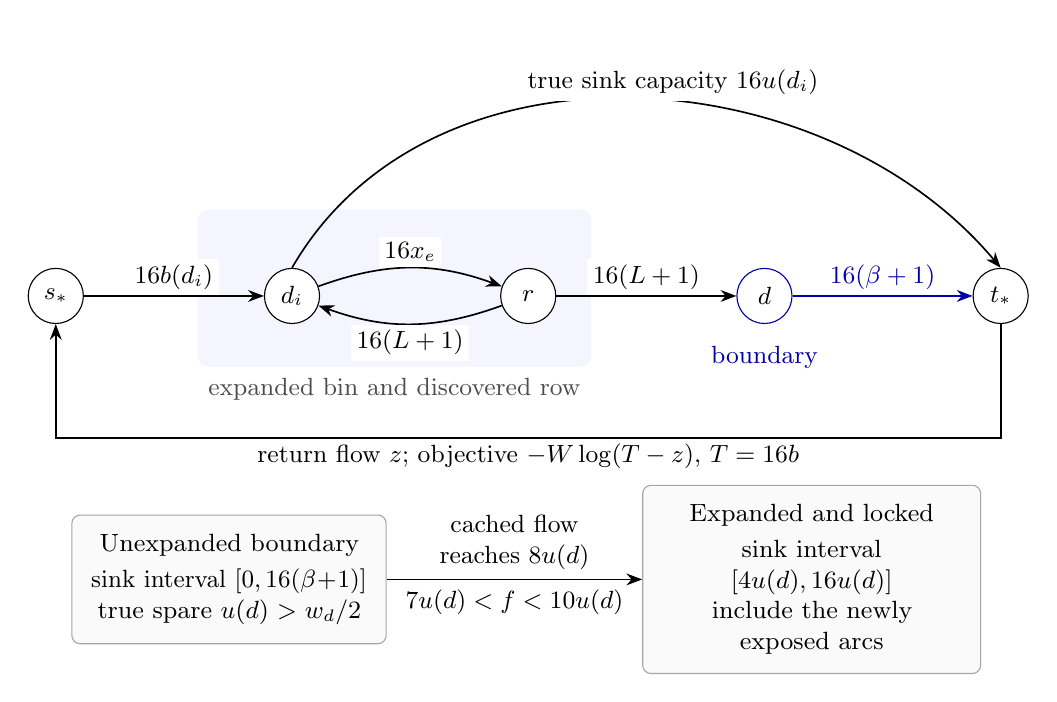
\begin{tikzpicture}[
    font=\small, >=Stealth,
    vertex/.style={circle,draw,fill=white,minimum size=7mm,inner sep=1pt},
    arc/.style={->,semithick},
    capacity label/.style={fill=white,inner sep=2pt},
    panel/.style={draw=black!35,rounded corners=3pt,fill=black!2,
      align=center,inner sep=7pt}
  ]
    \fill[blue!4,rounded corners=4pt] (1.8,-.9) rectangle (6.8,1.1);
    \node[anchor=north,text=black!70] at (4.3,-.92)
      {expanded bin and discovered row};
    \node[vertex] (s) at (0,0) {$s_*$};
    \node[vertex] (di) at (3,0) {$d_i$};
    \node[vertex] (r) at (6,0) {$r$};
    \node[vertex,draw=blue!65!black] (db) at (9,0) {$d$};
    \node[vertex] (t) at (12,0) {$t_*$};
    \node[anchor=north,text=blue!65!black] at (9,-.52) {boundary};
    \draw[arc] (s) -- node[capacity label,above] {$16b(d_i)$} (di);
    \draw[arc] (di) to[bend left=20]
      node[capacity label,above] {$16x_e$} (r);
    \draw[arc] (r) to[bend left=20]
      node[capacity label,below] {$16(L+1)$} (di);
    \draw[arc] (r) -- node[capacity label,above] {$16(L+1)$} (db);
    \draw[arc,blue!65!black] (db) --
      node[capacity label,above] {$16(\beta+1)$} (t);
    \draw[arc] (di.north) to[out=60,in=130]
      node[capacity label,above,pos=.55] {true sink capacity $16u(d_i)$} (t.north);
    \draw[arc] (t.south) -- (12,-1.8) --
      node[capacity label,below] {return flow $z$; objective $-W\log(T-z)$, $T=16b$}
      (0,-1.8) -- (s.south);

    \node[panel,text width=3.5cm] (optimistic) at (2.2,-3.6)
      {Unexpanded boundary\\[2pt]
       sink interval $[0,16(\beta+1)]$\\
       true spare $u(d)>w_d/2$};
    \node[panel,text width=3.8cm] (locked) at (9.6,-3.6)
      {Expanded and locked\\[2pt]
       sink interval $[4u(d),16u(d)]$\\
       include the newly exposed arcs};
    \draw[arc] (optimistic.east) --
      node[above,align=center] {cached flow\\reaches $8u(d)$}
      node[below] {$7u(d)<f<10u(d)$} (locked.west);
  \end{tikzpicture}
  \caption{The local threshold network and the boundary transition in
    Lemma~\ref{lem:projection}. Labels on ordinary arcs are scaled upper
    capacities; omitted unpadded lower bounds are zero. The schematic shows
    one expanded incidence and one boundary incidence. Initially all seeds
    $p_d\ge w_d/2$, and therefore all deficit bins, are expanded. A boundary has no
    outgoing bin-to-row arcs and no positive source capacity until expansion.
    Padded bounds are used by the engine. Expansion keeps the current flow
    and installs a permanent lower lock. If the last step succeeds before a
    new trigger is served, its boundary flow still satisfies
    $f<10u(d)<16u(d)$, so the true sink capacity is respected up to padding.}
  \label{fig:local-projection}
\end{figure}


Start each pad at \(4\delta\).  If a cached argument is at most
\(3\delta\), increase its pad by \(4\delta\) and re-anchor that
coordinate.  Explicit changes of bounds also re-anchor it.
Increasing a pad only increases the objective.  The register and
step-size guarantees, exactly as in Lemma~\ref{match:top-maintenance},
keep all ordinary arguments above \(\delta\) before a new step and
above \(\delta/10\) at a refresh after motion.  A serviced side does
not need another increase without further motion or a change of
its bounds.  The repairs can therefore be made on dirty and newly
inserted coordinates, without a scan of the represented graph at
each step.

The loose iteration and operation caps give, on every guarded
prefix, a total sum of pads
\begin{equation}
\label{proj:pad-budget}
             \alpha:=\sum_{e\ {\rm ordinary}}
                            (\zeta_e^-+\zeta_e^+)<S^{-800}.
\end{equation}
One may bound the number of potential repairs using all \(O(S)\)
ordinary arcs of the full exchange graph; locality is not needed
for this preliminary numerical estimate.  Alternatively, the
external-operation cap gives at most a fixed multiple of \(S^{100}\)
pad settings, each of size \(O(\delta)\), which is smaller than the
right side of \eqref{proj:pad-budget} for large \(S\).
There is no intervening infinite repair chain: a repaired argument
is exactly re-anchored, and the current point does not move during
the service.
All ordinary unpadded-bound violations sum to at most \(\alpha\).
Conservation at the source gives
\begin{equation}
\label{proj:return-range}
                     -\alpha\le z\le16\beta+\alpha .
\end{equation}

At each loop test read \(z\) exactly.  Stop successfully when
\(z\ge T-1/4\).  Otherwise the next step cannot cross \(T\):
the return contribution to its length is
\(W|\Delta z|/(T-z)\), and the step's total length is at most
\(q/100\).  Thus its relative return-argument change is at most
\(q/(100W)\).  In particular even the final successful step leaves
\begin{equation}
\label{proj:return-margin}
                              T-z\ge1/8 .
\end{equation}

\paragraph{Boundary locks and explored size.}
Before taking another pricing step, expand any boundary whose
cached sink flow is at least \(8u(d)\).  Replace its unpadded
optimistic sink interval by
\begin{equation}
\label{proj:lock}
                              [\,4u(d),16u(d)\,] .
\end{equation}
Retain this lower lock for the rest of the threshold test, and add
the newly discovered arcs with flow zero.  Pads can be
reinitialized when the sink bounds change.

The transition is interior with a constant margin.  At the start
of a step, an untriggered boundary has actual flow less than
\(8.2u(d)\): apply the register-error inequality to its
padded-zero lower argument and use \(u(d)\ge1\).
During the step its absolute change is at most
\((q/100)(F_e+\zeta_e^-)\), so its resulting flow is less than
\(10u(d)\).  At a first trigger the same cache guarantee gives
actual flow greater than \(7u(d)\).  Hence the new interval
\eqref{proj:lock} is safely interior.  Triggers are checked on
dirty or newly supplied entries using their latest registers.
Re-anchoring without motion cannot invalidate the estimate.
In particular, if success is detected immediately after a step,
before a newly triggered boundary has been serviced, that boundary
still has
\begin{equation}
\label{proj:unserviced-exit}
                              F_e<10u(d)<16u(d).
\end{equation}
Thus a successful exit does not require an uncharged final scan or
expansion.

Every previously locked sink carries at least \(4u(d)\), apart
from its pad violation; each just-triggering sink carries more
than \(7u(d)\).  All other sink flows are nonnegative apart from
their pad violations, and their sum is \(z\).  Equations
\eqref{proj:return-range} and \eqref{proj:boundary-spare} therefore
bound the total weight of nonseed expanded or triggering bins by
\(8P+1\).  Including seeds, the expanded weight is at most
\begin{equation}
\label{proj:region-size}
                              11(P+1).
\end{equation}
This also bounds physical scanning: an expanded bin has \(2w_d-1\)
vertices of degree at most three.  Per unit of expanded weight
there are at most six bin-to-row incidences, at most eighteen
row-to-bin incidences, and at most eighteen boundary occurrences.
Including source and sink arcs, there are fewer than
\(1000(P+1)\) ordinary arcs.  Each is inserted once, the region only
grows, and each sink is locked at most once.  The same bound thus
controls cumulative topological insertions in this test.

\begin{lemma}[Threshold certificate]
\label{proj:threshold}
An unfailed, nonsuspended threshold test cannot report
\(\mathrm{LOW}\) if the unlocked optimistic maximum is at least
\(T\) in scaled units.  Its success exit implies that the explored
true unscaled maximum is at least \(b\).
\end{lemma}

\begin{proof}
First impose the current integral ordinary bounds, including the
locks, and return interval \([0,16\beta]\).
The current point is exactly conserved.  Its ordinary violation
is at most \(\alpha\), and
\eqref{proj:return-range} adds at most \(\alpha\) more for the
return interval.  The total is at most \(2\alpha<1\), not merely
the ordinary-arc error.  Lemma~\ref{prelim:small-violation} supplies
an exactly feasible integral circulation for these bounds.

Starting from its ordinary flow, one can attain the unlocked
optimistic maximum while preserving all sink locks.  If the
present value is smaller, the ordinary residual network contains
a source-to-sink path; erase cycles to make that path simple.
The only additional lower bounds are on incoming sink arcs.
Their reversals leave the sink and cannot occur on a simple
source-to-sink path.  Every augmentation therefore preserves
the locks, even if the starting flow contained cycles.
This constructs, existentially, a feasible comparator
\((F',z')\) with \(z'\ge T\).

The difference from the current point is a nonzero circulation.
For each ordinary logarithmic term, a negative directional
derivative has magnitude at most one, since the comparator is
feasible even without the pads.  There are fewer than
\(2000(P+1)\) such terms.  The return term contributes
\[
                 \frac{W(z'-z)}{T-z}\ge W
\]
positively.  If \(A_+\) and \(A_-\) are the sums of positive and
absolute negative individual contributions, then
\[
 A_+\ge20000(P+1),\qquad A_-<2000(P+1),\qquad
 \frac{g^{\mathsf T}(F'-F,z'-z)}
      {\|\lambda(F'-F,z'-z)\|_1}
       =\frac{A_+-A_-}{A_++A_-}>\frac12 .
 \]
Only a direction is being compared; evaluating the logarithmic
objective at \(z'\ge T\) is neither intended nor necessary.
Lemma~\ref{lem:priced-steps} rules out \(\mathrm{LOW}\).

At a success exit, replace the optimistic boundary capacities by
the true ones and impose return interval \([T,16\beta]\).
Equation~\eqref{proj:unserviced-exit} shows that no unexpanded
boundary violates its true upper capacity, even before trigger
service.  There are no unexpanded deficits.  The ordinary
violation is at most \(\alpha\); the additional return violation
is at most \(1/4+\alpha\).  The total is less than one.
Lemma~\ref{prelim:small-violation} gives a feasible integral scaled
flow of value at least \(T=16b\) in the explored true graph.
Dividing capacities and flow value by \(16\) proves that its
unscaled maximum is at least \(b\).
\end{proof}

Continue until success, \(\mathrm{LOW}\), detected stochastic
failure, or suspension.  On \(\mathrm{LOW}\), verify by a static
integral maximum-flow computation that the unlocked optimistic
unscaled maximum is below \(b\).  On success, verify that the
explored true unscaled maximum is at least \(b\).
A contradictory exact check causes suspension; Lemma~\ref{proj:threshold}
shows that it cannot occur in an unfailed proceeding
computation.  These calls use
Lemmas~\ref{lem:integral-flow} and~\ref{lem:capacity-scaling}
with size padded to \(O(P+B)\).  Capacity digit scaling in
particular avoids a variable polynomial-capacity exponent when
\(P\) is small relative to \(S\).

Thus each verified test decides the threshold for the full graph.
On \(\mathrm{LOW}\), optimistic domination implies that the full
maximum is below \(b\).  On success, the explored true graph embeds
into the full graph and supplies value at least \(b\).
The locked engine network is discarded after the test; the exact
checks use the unlocked optimistic or true capacities, respectively.

\paragraph{Termination and cost of one test.}
The objective range at loop and service states is
\(O_a((P+1)\log S)\).  There are \(O(P+1)\) ordinary terms with
arguments between \(\delta/10\) and a guarded polynomial upper
bound, and the weighted return term has the same total order by
\eqref{proj:return-margin} and \(W=O(P+1)\).
Pad increases never lower the objective.  An arc insertion or a
lock change costs at most \(O(\log S)\) in objective, and there
are only \(O(P+1)\) such touches.  The
\(\Omega(q^2)\) increase per successful priced step consequently
bounds their number by
\begin{equation}
\label{proj:step-count}
                    O_a((P+1)q^{-2}\log S).
\end{equation}
Use, for example, nominal engine lifetime size \(8192(P+1)\),
including every new endpoint and arc.  Point reads of the return
arc, local pad changes, boundary notifications, and the final
static verification are charged.  No global scan is made at a
pricing step.  Lemma~\ref{lem:priced-steps} and its notification
bound now give \eqref{proj:time} for one threshold.  The guard
\(S^{20}\) on local pricing iterations is eventually larger than
\eqref{proj:step-count} because
\(q^{-2}=O_a(S^{200/a})\) and \(P=O_a(S)\).

\paragraph{Recovering the exact flow and the full peel.}
The threshold tests determine the maximum value, but the matching
procedure also needs the exact allocation changes and, when a deficit
remains, the entire residual source-reachable bin set.  We now recover
this information from the small regions explored by the tests.

\begin{lemma}[Recovering the full residual cut]
\label{proj:local-cut}
Suppose \(\beta>0\), and let \(v\) be the full unscaled exchange maximum.
Suppose a true
explored region of maximum \(v\) is available when \(v>0\), and
an unlocked optimistic region of maximum \(v\) is available when
\(v<\beta\).  The union of the available regions, using true
capacities and original arc identifiers, suffices to compute an
exact full exchange flow and, when \(v<\beta\), the full residual
source-reachable bin set.
\end{lemma}

\begin{proof}
Call the supplied true region the success graph and the supplied
optimistic region the failure graph.  Suppose \(v<\beta\), and
let \(Q\) be a minimum source side of the failure graph.
No boundary belongs to \(Q\), because its
sink arc alone has capacity \(\beta+1>v\).  Consequently every
bin of \(Q\) is expanded and all its outgoing bin-to-row arcs of
positive true capacity are represented.  Every represented row
has all its outgoing row-to-bin arcs, and every positive source
arc is present because all deficits are seeded.  Thus all arcs
leaving \(Q\) in the full true graph occur with the same capacity
in the failure graph.  The same set \(Q\) is a full-graph cut
of capacity \(v\).

The true success graph supplies value \(v\) when \(v>0\).
Solve an exact integral maximum flow in the union with true
capacities, using the failure graph alone when \(v=0<\beta\),
or the success graph alone when \(v=\beta>0\).
The union's value is exactly \(v\), by the cut just proved or by
the total source capacity \(\beta\).
Extend its flow by zero to the full network.

When \(v<\beta\), equality of its value with the capacity of
\(Q\) forces every outgoing cut arc to be saturated and every
incoming cut arc to have zero flow.  Neither an unsaturated
forward arc nor a positive-flow reverse arc can leave \(Q\).
All positive-capacity original arcs needed within \(Q\) are
represented, and every needed reverse arc is the reverse of
an arc carrying positive flow in the union.
Residual reachability computed in this local representation is
therefore the full residual source reachability.  Its bin part
is precisely \(R_0\).
\end{proof}

\begin{proof}[Proof of Lemma~\ref{lem:projection}]
List the positive parent debts to find the seeds and compute
\(\beta\), in \(O(P)\) point operations.  If \(\beta=0\), the
unchanged allocation already satisfies the requested floor, so
giving the fresh child an empty debt map finishes the projection.
The parent ledger remains unchanged.

Otherwise binary search, using the verified threshold tests,
determines the full unscaled maximum \(v\).  Retain a true success
graph for \(v\) when \(v>0\).  If \(v<\beta\), retain an optimistic
failure graph for \(v+1\).  Its unlocked maximum is exactly \(v\):
it is below \(v+1\) by the test, at least \(v\) by optimistic
domination, and integral.  At most a constant number of additional
tests retrieves these regions.  Lemma~\ref{proj:local-cut} then
returns the exact flow and, when needed, its full residual bin set.

The union has size \(O(P+1)\).  Its flow support supplies all
allocation changes.  The set \(R_0\) has weight \(O(P)\), either
by \eqref{proj:region-size} or by applying the parent deletion
inequality to the failed floor-\(c\) projection.  Listing its
assigned rows and their affected allocations requires only
that physical weight and bounded row degree.  No scan of an
unexpanded high-volume bin or of an unchanged parent allocation
is necessary.  This completes the local construction.
There are \(O(\log S)\) thresholds and retrieval tests because
\(\beta\le P=O_a(S)\).  The per-test bound \eqref{proj:time},
the final static flow on the union, and these sparse ledger changes
give the asserted total time.  Each reached priced-step instance
has its stated conditional failure allowance; a detected failure
or suspension is returned to the caller immediately.
The numerical and nominal-size prerequisite checks, including
those used above, are justified uniformly on guarded prefixes
in Lemma~\ref{phase:guard-adequacy}.
\end{proof}

\subsection{Debt, structural work, and progress}

The following estimates apply before the first deterministic
interruption, and do not assume that the graph has a perfect
matching.  A detected failure terminates the test; a returned
structural action or projection satisfies its deterministic
invariants.

\begin{lemma}[Phase accounting]
\label{phase:accounting}
In a phase with initial deficit \(K\), threshold \(L\), and target
\(g_*\), every guarded prefix before completion satisfies
\begin{equation}
\label{phase:peel-budget}
 \sum_{\rm peels}w(R_0)\le2L(g_*-1)+S^{-800},
 \qquad
 \#\{\text{blockers}\}\le2C(g_*-1).
\end{equation}
There are \(O(N+Lg_*)\) expansions, the sum of contraction
arities \(|X|\) is \(O(N+Lg_*)\), and the total tick increase is
\(\tau=O_a(N)\).
\end{lemma}

\begin{proof}
Before the terminal \(g_*\)-th gain there are at most \(g_*-1\)
gains whose ledgers are repaired.  Top contractions preserve
total debt, top expansions consume available slack without
other debt, and the positivity service of
Lemma~\ref{match:top-maintenance} adds less than \(S^{-800}\) debt.
By Lemma~\ref{match:deletion}, each repaired gain adds at most \(2L\)
net debt.  By Lemma~\ref{match:exchange-projection}, every projection
peel consumes at least its weight from the top ledger.
Nonnegative remaining debt gives the first bound in
\eqref{phase:peel-budget}.

The number of new blockers at a peel is at most
\(h(R_0)<Cw(R_0)/L\).  Summing this strict inequality and using
integrality gives the second bound in
\eqref{phase:peel-budget}; the tiny positive remainder is less
than one.  In particular, before the first gain of a phase
with \(g_*=1\), no positive-weight peel can occur.

The bottom certificate of Lemma~\ref{match:bottom-surplus} bounds the
weight removed by a gain by \(2L\).
A removed bin has \(2w_d-1\) physical vertices, and at most one
assigned row per removed bin is materialized with it.  Thus the
number of vertices returned to the paired remainder is bounded
by a constant times the total erased weight.  Every expansion
consumes a pair from that remainder.  Its initial population is
at most \(N\), so expansions number \(O(N+Lg_*)\).
Initially there are at most \(N\) bins and each expansion creates
one new bin.  A contraction decreases their number by
\(|X|-1\), and \(|X|\ge2\); hence the sum of \(|X|\) over
contractions is also \(O(N+Lg_*)\).
Expansions and contractions contribute one tick each, and a
repaired gain contributes \(L\), giving
\(\tau=O(N+Lg_*)\).

Finally \(Lg_*=O_a(N)\).  If \(K<100C\), then \(g_*=1\) and
\(L=O_a(N)\).  Otherwise
\[
 Lg_*\le
 \left(\frac{10000CN}{K}+1\right)\frac{K}{100C}
 =O(N).
 \]
This proves the tick bound.
\end{proof}

\begin{lemma}[No false stall without a stochastic failure]
\label{phase:stall}
If the subcubic graph has a perfect matching, a settled phase
state with fewer than \(g_*\) gains admits neither a valid
\(\mathrm{LOW}\) exit nor a permanent lack of progress.
More precisely, when neither a distinct-bin contact nor an
eligible expansion is available, the top objective has a
circulation direction \(d\) with
\[
                      g^{\mathsf T}d
                           >\tfrac12\|\lambda d\|_1 .
 \]
\end{lemma}

\begin{proof}
Let \(i_*\le g_*-1\) be the gains so far.
For this argument only, realize the matching represented by the
partition.  This is an existence comparison, not an instruction
to materialize the graph at every pricing step.
Taking the symmetric difference with a perfect matching gives \(K-i_*\)
vertex-disjoint augmenting paths~\cite{Berge1957}.  At most the blocker count
meet a blocker.

Orient each remaining path from an unmatched endpoint.
Its first bin is free and is entered at its exposed base.
That bin has no other unmatched vertex and no crossing matching
edge.  At a stall there is no edge to a distinct bin.
If the path exits to a row by a nonmatching edge, its next
matching edge is that row's assigned edge, entering another
bin at its base.  This new bin is assigned; its only possible
crossing matching edge is the one just used on entry.
A simple path must therefore next exit it by a nonmatching
edge.  Continuing this argument, the path must eventually
reach \(U\): it avoids blockers, cannot end inside an assigned
bin, and cannot enter another free bin through an assigned
row edge.

Every such entry uses the unique physical base of its bin.
Simplicity and vertex-disjointness consequently imply that
the prefixes through their first \(U\)-contacts use distinct
bins and rows, both within a prefix and across different
prefixes.  Reassign each prefix row to the preceding bin in
its chain.  This is simultaneously injective and frees the
last bin of every prefix.
If \(Z\) denotes all bins with a \(U\)-contact, one can thus
leave simultaneously free a subset of \(Z\) of size
\begin{equation}
\label{phase:free-contacts}
 r\ge K-i_*-2C(g_*-1)\ge K/2 .
\end{equation}

Scale this conceptual assignment by \(L\).
The desired top column capacities are
\[
                         L+p_d^0-Cw_d ,
\]
which are nonnegative because the current top allocation and
positive slack realize them.  Clip overloaded columns by
removing mass.  An assigned column initially carries \(L\),
so its removed mass is at most \(Cw_d\); the total removed is
at most \(Cw(\mathcal D)\le CN\).
The current top allocation proves that all rows can be filled
under these capacities.  Complete the clipped partial
transportation flow by residual source-to-sink augmentations;
one can scale the dyadic data and use integral path
decomposition for this existence argument.  Simple augmenting
paths do not leave the sink, so column sink flows do not
decrease.  The \(r\) initially empty specified columns receive
in total at most the removed mass.
The resulting allocation \(x'\) has nonnegative slacks \(s'\)
and satisfies
\begin{equation}
\label{phase:alternative-slack}
                           s'(Z)\ge Lr-2CN .
\end{equation}

At a stall, the cache-based eligibility guarantee of
Lemma~\ref{match:top-maintenance} gives \(s_d\le5C\) on \(Z\).
Take the difference from the current allocation and slack as
a direction.  Row sums and column equations are unchanged,
so it is a circulation in the top engine graph.
Every negative individual logarithmic directional contribution
has magnitude at most one, since \(x',s'\ge0\).
Their total is at most
\(|E(\mathcal B)|+|\mathcal D|\le4N\).
The positive sum is at least
\[
 \frac{s'(Z)}{5C}-|Z|
 \ge \frac{Lr-2CN}{5C}-N .
 \]
By \eqref{phase:free-contacts} and
\(L\ge10000CN/K\), this is greater than three times \(4N\).
As \(\lambda\) counts the absolute individual contributions,
the claimed ratio is greater than one half.
Lemma~\ref{lem:priced-steps} excludes \(\mathrm{LOW}\) unless
it explicitly reports failure or suspension.  Its positive
objective increase, with the bounded objective accounting
below, also excludes indefinite pricing without another
structural action.
\end{proof}

\subsection{Implementation and total phase cost}
\label{phase:implementation}

We give the representation and cost details needed to sum the
local work.  The charges are to touched records and actual
engine notifications, rather than to a whole graph per event.

\paragraph{Physical structure.}
Maintain physical vertices, bin and row identifiers, mates,
assignments, incident lists, and edge classifications in
dictionaries and linked lists.  Maintain a set of distinct-bin
contacts and, for each bin, a list of contacts to \(U\) with
its first member accessible.  A register refresh changes a
bin's eligibility flag without scanning its contacts.

At a contraction retain a largest old bin's representative.
Move the smaller bins' member lists and the swallowed rows,
updating their physical incidences and affected ledger
records.  Unchanged exterior incidence allocations retain
their values and need only endpoint retargeting when
necessary.  Sum bin data using \(|X|\) point reads per
retained ledger; do not scan the largest bin's members.
A moved old member's bin size at least doubles during its
uninterrupted stay in bins.  Initial membership, new
expansions, and swallowed row entries begin new charges;
erasures and later returns are covered by
Lemma~\ref{phase:accounting}.  Deletions inspect only removed
bins, their assigned rows, and their affected physical
incidences, applying Lemma~\ref{match:deletion}.
Subcubicity therefore bounds all physical structural touches,
including endpoint retargeting, by
\begin{equation}
\label{phase:structural-touches}
                         O_a((S+Lg_*)\log S).
\end{equation}
Assignment flips in the pair primitive require only abstract
assignment updates.  By Lemma~\ref{match:pair-action}, successful
contractions charge their abstract arity, gains charge \(L\)
up to logarithmic factors, and a final abort costs at most
that latter amount.  All bin-pair work is consequently
\begin{equation}
\label{phase:pair-work}
                    O_a((S+Lg_*+L)\polylog S),
\end{equation}
with the fixed reliability factors included.  Materialization
uses Lemma~\ref{match:materialization} and is charged by the same
physical erasure work or by one final phase-boundary scan.

\paragraph{Top values and objective.}
At a structural edit, read and reset only the affected top
coordinates.  The top column residual is available from
\[
                         y_d^0=s_d-p_d^0+Cw_d ;
\]
it does not require a separate global sum of implicitly
moving allocations.  The aggregation, redirection,
restriction, and tiny transfers determine affected slacks
exactly, preserving column equations without rounding.
Compute all final settings of a batch before submitting
deletions, point changes, and insertions to the engine.
Both old and newly anchored descriptors then have positive
arguments, and no pricing call occurs until the completed
topology again satisfies its equations.
Notifications arising during this service can be queued:
there is no implicit primal motion during the service.
Settle all dirty small-argument and eligibility checks
before choosing the next main action.

Use nominal top-engine lifetime size \(SB\), with an explicit
check on the representation.  Only actual topological
insertions and retargetings consume new incidence slots;
repricing, motion, and positivity repairs on retained
coordinates do not.  Equation~\eqref{phase:structural-touches}
makes this nominal bound sufficient eventually.
For fixed \(a\), Lemma~\ref{phase:accounting} gives
\[
 L=O_a(S),\qquad
 \sum_d p_d^0=O_a(Lg_*+1),\qquad
                         s_d\le L+\sum_d p_d^0 .
\]
Thus at pricing states all top arguments lie in a range
whose logarithmic width is \(O_a(\log S)\), and there are
only \(O(S)\) coordinates.  The top objective range is
\(O_a(S\log S)\).  Each affected coordinate at a structural
edit costs at most \(O_a(\log S)\) in objective, so the
cumulative structural loss is
\(O_a((S+Lg_*)\log^2 S)\).
The donor decrease in a tiny positivity transfer has loss
\(O(\delta)\), and its total is already covered by the
tiny-repair count.  Each successful priced step increases
the objective by \(\Omega(q^2)\).  Hence their number is
\begin{equation}
\label{phase:top-step-count}
                             O_a(Sq^{-2}\log^2 S).
\end{equation}
Dirty-entry repairs and eligibility work charge a constant
number of point operations per notified or structurally
touched entry.  The notification bound of
Lemma~\ref{lem:priced-steps} and
\eqref{phase:top-step-count} put the total top work in
\(S^{1+O(1/a)+o_a(1)}\).

\paragraph{Persistent integral ledgers.}
Store allocations by physical incidence and \(y,p\) by bin
in persistent point maps, for example path-copy balanced
trees.  Maintain an index and sum of positive live debts;
deleted keys are cleared, and new bins are initialized
locally.  Retained levels receive their structural edits
separately.  At a projection from integral parent \(j-1\),
retain the parent's roots from \emph{before} a possible
peel, and modify a copy only along the obtained flow support
and deletions.  Include the exterior loads freed by removed
rows.  The new child's debt map is empty.  Apply preserving
deletions separately to coarser ledgers, and let all deeper
fresh ledgers initially share the new child's roots.
This costs local projection-size work and logarithmic
record overhead, not a whole-vector copy at each reset.
Level \(1\) may build entire maps after its global static
flow computation.

The reset periods of Section~\ref{match:reset} are
\(b_j=B^{a-j}\).
Suppose an event selects level \(j>1\).  Even if the event
advances ticks by \(L\), it crosses no \(b_{j-1}\) boundary:
otherwise a coarser reset would have been selected.
Its integral parent last reset to zero debt in this same
\(b_{j-1}\) period interval; every crossing of such a
boundary resets that parent or a coarser ledger.
Its debt rises by at most \(C\) per expansion and \(2L\)
per gain, and never positively for another action.
Since these actions advance ticks by \(1,L\), respectively,
the debt at the triggering event obeys
\begin{equation}
\label{phase:parent-debt}
                              P\le(C+2)b_{j-1}.
\end{equation}
This reasoning uses both the pre-event and post-event
quotients, so a jump over several periods cannot defeat it.
In particular \(P=O_a(S)\) for \(j>1\).

At most \(\lfloor\tau/b_j\rfloor\) events select level \(j\):
each can be charged to a distinct crossed \(b_j\) boundary.
By \(b_{j-1}/b_j=B\), Lemma~\ref{lem:projection}, and
\eqref{phase:parent-debt}, all \(j>1\) projection costs sum to
\begin{equation}
\label{phase:local-reset-sum}
 \sum_{j=2}^a
   \frac{\tau}{b_j}\bigl((C+2)b_{j-1}+B\bigr)
                    S^{O(1/a)+o_a(1)}
       =S^{1+O(1/a)+o_a(1)} .
\end{equation}
The small-instance padding \(B\) is included here.
For level \(1\), the global exact exchange computation has
cost \(S^{1+o(1)}\).  Since
\(b_0=B^a\ge S\) and \(b_1=b_0/B\), its total is at most
\[
                  \frac{\tau B}{S}S^{1+o(1)}
                         =S^{1+O(1/a)+o_a(1)} .
\]
Together with initialization and the preceding charges,
this proves the desired phase cost on completed guarded
prefixes.

\subsection{Guarded prefixes and the PM guarantee}

\begin{lemma}[Eventual adequacy of the guards]
\label{phase:guard-adequacy}
For every sufficiently large fixed \(a\) and fixed
admissible reliability parameter \(\sigma\), all deterministic
guards of the PM construction are adequate for all
sufficiently large \(S\), on every computation path.
The bounds just proved apply also to a prefix ending in a
failed or interrupted attempted operation.  No perfect-matching
promise is needed for these time and adequacy assertions.
\end{lemma}

\begin{proof}
Consider the prefix through a putative first deterministic
interruption.  The elementary initial checks, such as
\[
 S\ge2^{100},\qquad
 100000C,\ B\le S^{1/20},\qquad q\ge S^{-1},
\]
are eventually satisfied at each fixed sufficiently large
\(a\).  The loose \(S^{20}\) iteration caps and the
\(S^{100}\) external-operation cap suffice first to bound
tiny positivity debt and local pads.  A small argument
increased and exactly re-anchored does not require another
increase without motion or a reset of its bounds.  A top
donor is chosen exactly from a bounded-degree row with sum
\(L\); local repair does not create an unbounded chain of
new small donors.  Thus these numerical error estimates
do not assume the sharper running-time bounds that they
are used to prove.

All completed structural actions and peels preserve the
deterministic ledger and matching invariants.  Their debt
payoffs and the bottom certificates prove
Lemma~\ref{phase:accounting} independently of objective
progress.  Include the present structural action if any.
For a coarse numerical bound, one has
\[
 L\le10000CS+1,\qquad g_*\le S,\qquad
 \text{erased weight}\le4Lg_*+1,
\]
and at most \(N+4Lg_*+2\) expansions, allowing the next
one as well.  Every retained integral ledger has acquired
at most
\begin{equation}
\label{phase:crude-debt}
                      C(N+4Lg_*+2)+2Lg_*
\end{equation}
debt between its resets, even without using
\eqref{phase:parent-debt}.  Column loads are at most
\(L|\mathcal A|\).
Together with \(100000C\le S^{1/20}\), these estimates put
all top data, exchange capacities, local return weights
and scaled capacities, and argument upper bounds well
inside \(S^{20}\).
Thus numerical adequacy does not depend on
parameter-dependent rounding constants in the period bound.

At a local threshold test, the current sink consumption
already bounds every lock-trigger expansion by
\eqref{proj:region-size}, before that expansion is
performed.  Ready arguments and post-motion refreshes have
the required lower margin, and explicit edit batches use
positive old and final settings.
At the top, \eqref{phase:structural-touches}, with one
extra physical-size edit allowance, verifies the nominal
lifetime bound \(SB\) at a possible first overflow.
At a local test, \eqref{phase:parent-debt} and its
\(8192(P+1)\) nominal size give the engine condition
\(R+B\le S^{1+2/a}\) eventually.  The same is true for
the top nominal size.

The structural and objective estimates
\eqref{proj:step-count} and \eqref{phase:top-step-count}
bound all completed iterations.  Add at most one final
\(\mathrm{LOW}\), failed, or interrupted attempt.
Because \(q^{-2}=O_a(S^{200/a})\), these bounds remain
below \(S^{20}\) for fixed sufficiently large \(a\) and
large \(S\).
Up to a hypothetical first external-operation cap,
the engine's notification bound charges dirty coordinates
to priced motion.  Client repairs add only constantly
many point operations per dirty trigger, besides the
structural edits, and have no no-motion repair chain.
Consequently even this cap-reaching prefix has only
\(S^{1+O(1/a)+o_a(1)}\) external work, eventually smaller
than \(S^{100}\).  The priced-step lemma's own eventual
prerequisite adequacy applies within these hypotheses.

These arguments are uniform over successful verified
states and rejected stochastic attempts.  The engine
lemma bounds attempted operations on every path; its
construction uses verified structures and capped failed
attempts, not a good-event-only time estimate.
The pair primitive likewise either returns a valid
action within its charged bound or terminates negatively.
A detected stochastic failure promptly ends the PM test,
whereas an inadequate deterministic prerequisite suspends
the branch.  The latter has just been excluded in the
fixed-parameter asymptotic range.  All local scans and
updates, including a final pair abort or incomplete
attempt, are charged by their represented work.
This proves the claim.
\end{proof}

\begin{theorem}[Fixed-parameter subcubic perfect-matching search]
\label{thm:subcubic}
For the integers \(a\ge1000\) and fixed reliability parameters
\(0\le\sigma\le a+1\), the construction defines a uniform
randomized algorithm on loopless subcubic graphs with
identified edge copies and \(N\le S\) vertices.
Every computation halts with a checked perfect matching,
a negative answer, or a suspension.
It has no false positive.
For each fixed input with a perfect matching, the
probability of a negative answer is at most
\begin{equation}
\label{phase:pm-error}
                            2^{-\sigma}S^{-5}.
\end{equation}
This statement bounds erroneous answers, not suspensions,
and holds conditionally for adaptive invocations with
fresh randomness and valid prerequisites.

For every sufficiently large fixed \(a\) and fixed
admissible \(\sigma\), there is no suspension on any path
at all sufficiently large \(S\).  The total time on every
path is then
\begin{equation}
\label{phase:pm-time}
                              S^{1+O(1/a)+o_a(1)},
\end{equation}
where the exponent coefficients in \(O(1/a)\) are
absolute.  All initialization, physical data movement,
arithmetic, random bits, and explicit witness writing
are included.
\end{theorem}

\begin{proof}
Settle trivial cases directly; an odd number of vertices
has no perfect matching.  Start with the empty matching
and run the phase construction.  When
\(K\ge200C\), a completed phase gains at least
\(K/(200C)\).  Below that threshold, at most \(200C\)
further phases are needed, each gaining at least one.
Thus there are \(O_a(\log S)\) completed phases, and
at most one final negative or suspended phase.
Each has the bound established above.
Initialization, phase-boundary materialization, and the
final edge-identifier and vertex-coverage check cost
only the already allowed near-linear work.
Lemma~\ref{phase:guard-adequacy} makes
\eqref{phase:pm-time} an every-path bound and excludes
suspension in the stated asymptotic range.
On arbitrary checked sizes, the explicit iteration,
operation, representation, and sampling caps still give
halting, with suspension permitted.

On a PM instance, in the absence of a stochastic failed
guarantee or suspension, valid pair actions and
projections preserve the invariants.
Lemma~\ref{phase:stall} prevents a \(\mathrm{LOW}\)
negative answer before the phase target.  The objective
step bound prevents an infinite sequence of priced
steps, so each phase reaches its gains and the algorithm
eventually constructs a perfect matching.
Checking the proposed edge copies and coverage excludes
false positives on every input, including no-instances.

For the probability bound, count invocations using the
loose guards rather than conditioning on later
noninterruption.  There are fewer than \(S\) nontrivial
phases, at most \(S^{20}\) main actions per phase, and
only logarithmically many threshold tests and retrieval
tests per projection.  On these prefixes,
\[
                      \beta\le CN+L|\mathcal A|,
\]
so its search range has logarithmic bit length.
The total number of pair queries and priced-step
instances is, conservatively, less than \(S^{50}\).
Each reached pair query has the conditional error
allowance in Lemma~\ref{match:pair-action}; each reached
engine instance has the conditional allowance of
Lemma~\ref{lem:priced-steps}.  Both are at most
\(2^{-\sigma}S^{-60}\).
Union over the reached invocations gives at most
\(2^{-\sigma}S^{-10}\), which is smaller than
\eqref{phase:pm-error}.

The conditional bounds are applied when the invocation's
input and prerequisites are fixed by its past history,
and its new bits are fresh.  They are not conditioned on
whether the branch later suspends or wins a scheduling
race.  An additional deterministic suspension produces
no negative answer by itself.  This proves
\eqref{phase:pm-error} also at checked sizes where
suspension remains possible, and completes the theorem.
\end{proof}

\section{Priced logarithmic steps}\label{sec:engine}

This section constructs the optimization primitive used by the matching
algorithm and the local projection procedure.  The primitive maintains
exact values implicitly, while exposing sufficiently accurate coordinate
registers to its client.  Its progress guarantee depends on the length of
the actual path representation returned by a cycle data structure.  In
particular, cancellation in the resulting circulation does not reduce the
motion charged to a step or to a register refresh.

Approximate minimum-ratio circulations serve as optimization directions
in the almost-linear flow framework of Chen et al.~\cite{FlowRandomized}.
The step estimate below is proved for the logarithmic objective and the
raw-motion convention used here.

\subsection{The interface}\label{engine:interface}

Fix a master bound $S=2^s$ and integer parameters $a\ge1000$ and
$\sigma\ge0$.  Recall
\begin{equation}\label{engine:parameters}
 B=2^{\lceil s/a\rceil},\qquad q=B^{-100},\qquad
 \delta=S^{-1000},\qquad \varepsilon=S^{-3000}.
\end{equation}
Every asymptotic estimate in this section is for fixed parameters.  The
constants multiplying $1/a$ in exponents are absolute; an $o_a(1)$ term
may include logarithmic powers whose exponents depend on $a$ and
$\sigma$.  We use deterministic prerequisite checks, including
$q\ge S^{-1}$.  An inadequate prerequisite suspends the parameter branch
without producing an answer.  A detected stochastic failure is a distinct
outcome, with the probability bound stated below.

Let a changing oriented multigraph have real edge variables $f_e$ on the
grid $\varepsilon\mathbb Z$.  Loops and individual parallel edge copies
are allowed.  Its separable objective $\Phi(f)=\sum_e\phi_e(f_e)$ has one
of the following terms on each edge:
\begin{equation}\label{engine:objectives}
 \log f,\qquad
 \log(f-D_1)+\log(D_2-f),\qquad
 -W\log(T-f),\quad 1\le W\le S^{20},
\end{equation}
where $W$ is an integer.  The endpoints $D_1,D_2,T$ lie on the same grid
as the values.  Write $g_e=\phi'_e(f_e)$, and let $\lambda_e$ be the sum
of the absolute derivatives of the individual logarithmic terms on that
edge, including their weights.  Thus, for the two-sided term,
\[
 g_e=\frac1{f_e-D_1}-\frac1{D_2-f_e},\qquad
 \lambda_e=\frac1{f_e-D_1}+\frac1{D_2-f_e}.
\]
All data and values have magnitude at most $S^{20}$, and the positive
arguments at pricing and refresh states lie between $\delta/10$ and
$S^{20}$.  Small additional relative margins immediately after a step
are harmless in these bounds.  The applications maintain the stricter
pre-step margins established in the preceding sections.

The client may add, remove, or retarget edges and vertices, change a
descriptor or value on one coordinate, and request an exact point value.
Its explicit value settings need not be circulations.  Between such
edits, all increments performed by the primitive must be circulations.
The values themselves need not have zero divergence.

\begin{lemma}[Priced logarithmic steps]\label{lem:priced-steps}
Suppose a nominal bound $R$ counts the logical vertex and edge births and
endpoint insertions over one instance, including retargetings.  Mere
value or price changes on retained topology need not be counted as new
incidences.  Assume
\begin{equation}\label{engine:nominal-size}
                         R+B\le S^{1+2/a}.
\end{equation}
There is a uniform implementation with the following properties.
\begin{enumerate}[label=\textup{(\roman*)}]
\item A pricing call may return \textnormal{\textsc{Low}}, but it cannot do so if
there is a nonzero circulation $d$ satisfying
\begin{equation}\label{engine:high-direction}
                    g^{\mathsf T}d\ge\tfrac12\|\lambda d\|_1,
\end{equation}
unless it reports a detected failure or suspends.
\item A call not returning \textnormal{\textsc{Low}}, failure, or suspension performs
an exact increment $h\in\varepsilon\mathbb Z^E$ that is a circulation and
satisfies
\begin{equation}\label{engine:step-guarantee}
       \|\lambda h\|_1\le q/100,
       \qquad g^{\mathsf T}h\ge q^2/1000.
\end{equation}
It leaves all logarithmic arguments positive and increases $\Phi$ by
$\Omega(q^2)$.
\item The implementation exposes registers $\widehat f_e$.  After
settling updates and before the next pricing call, the descriptors are
valid at these registers and
\begin{equation}\label{engine:register-guarantee}
       \lambda_e(\widehat f_e)|f_e-\widehat f_e|\le q/100.
\end{equation}
An explicit client setting can reanchor the coordinate exactly.
Apart from such client settings, the number of refresh notifications is
at most the number of successful pricing steps times
$S^{O(1/a)+o_a(1)}$.  Notifications are supplied as a list of dirty
coordinates.  Maintaining the representation without taking a step
causes no implicit primal motion.
\item With $Q$ external pricing, point, and edge operations, total time,
excluding the client's own work, is
\begin{equation}\label{engine:time}
                     (R+B+Q)S^{O(1/a)+o_a(1)}.
\end{equation}
The bound is on every computation path and includes initialization,
arithmetic, random bits, and all representation changes.  Polynomially
many operations are allowed, with a loose guard $Q\le S^{100}$.
\end{enumerate}
The conditional probability of detected failure in the entire instance
is at most $2^{-\sigma}S^{-60}$, including when the instance is chosen
adaptively.  Deterministic size, precision, and representation checks may
suspend, but none does so for all sufficiently large $S$ at each
sufficiently large fixed $a$ and each fixed $\sigma\ge0$ within the
stated hypotheses.
\end{lemma}

The objective conclusion in part~\textup{(ii)} follows directly from its
two inequalities once positivity is established.  The sum of absolute
relative argument changes is at most $\|\lambda h\|_1$.  For a positive
logarithm, $\log(1+z)\ge z-z^2$ when $|z|\le q/100$; the sum of these
squared relative changes is at most $q^2/10000$.  A negative logarithm
in~\eqref{engine:objectives} is convex and lies above its supporting
tangent.  Hence the total increase is at least
$q^2/1000-q^2/10000$.

\subsection{A backend with explicit forest paths}\label{engine:backend-interface}

We use the following fully dynamic backend.  Its construction, rather
than a dynamic optimization oracle, is given in
Sections~\ref{sec:backend-quality} and~\ref{sec:backend-updates}.  The
minimum-ratio-cycle and hierarchical-routing viewpoint is related to
the flat-forest cycle machinery of~\cite{IncrementalGraphs}.  We give a
complete construction for the precise interface below, including its
raw path length and explicit forest recourse guarantees.

\begin{lemma}[Flat-cycle backend]\label{lem:flat-cycle}
Let $M=2^u$, where $u$ is divisible by $2a^2$, and suppose
\begin{equation}\label{engine:backend-size-range}
                         S^{1/a}\le M\le S^2.
\end{equation}
Consider a dynamic undirected graph with reference orientations and
fixed vertex slots, of total current size at most $M$ and maximum degree
at most three.  It has positive integral lengths $\ell_e$ and integral
signed gradients $\gamma_e$, both of magnitude at most $M^{1200a}$.
Insertions and deletions are arbitrary; a price replacement is a
deletion followed by an insertion.  Put
\[
 \OPT=\max_{d\ne0,\ d\text{ a circulation}}
          \frac{|\gamma^{\mathsf T}d|}{\|\ell d\|_1},
\]
with value zero if there is no nonzero circulation.

The backend exposes a forest.  Every forest vertex maps to an input
vertex slot; every forest edge either maps to a current input edge with
specified endpoint correspondence, or is null and joins equal images.
The multiplicity over each input slot is at most $M^{10/a}/4$.
A query returns a list of oriented single input edges and oriented
forest paths, the latter specified by endpoints.  Each piece is used
with unit multiplicity, with repeated pieces listed separately.  Their
signed physical projection is a circulation $c$.  Its \emph{raw length}
$V$ is the sum of input lengths over all mapped edge traversals with
repetition; a null forest traversal contributes zero.  If $\OPT>0$, the
answer has $V>0$ and
\begin{equation}\label{engine:flat-quality}
                   \frac{|\gamma^{\mathsf T}c|}{V}
                       \ge M^{-10/a}\OPT.
\end{equation}
An empty or missing answer is permitted when $\OPT=0$.
There are $M^{O(1/a)+o_a(1)}$ pieces in an answer.

Initialization costs $M^{1+O(1/a)+o_a(1)}$.  Amortized edit and query
costs, including explicitly exposed forest logs, are
$M^{O(1/a)+o_a(1)}$, with bounds on every path.  Retained forest
occurrences and edges have stable lifetimes.  Endpoint or mapping changes
are replacements, and removals are exposed before the old mappings or
input data are invalidated.  Transactions permit deletion-first
old-to-final updates with no intervening path query.

The bounds apply over the polynomial lifespans required by
Lemma~\ref{lem:priced-steps}, and against adaptive clients.  Reliability
can be chosen so that detected failure in an entire engine instance has
conditional probability at most $2^{-\sigma}S^{-60}$.  A flagged state
has no quality requirement.  Deterministic prerequisite checks may
suspend, with eventual adequacy as in Lemma~\ref{lem:priced-steps}.
\end{lemma}

\subsection{Degree reduction and integer pricing}\label{engine:pricing}

For each logical edge insertion, create a fresh port at each endpoint;
a loop receives two distinct ports.  The ports belonging to one logical
vertex lifetime form a path, extended on further endpoint insertions.
Retargeting uses fresh ports.  A retired port may remain on its path, and
a retired vertex may leave a wholly inactive path after all its real
incidences have disappeared.  Distinct vertex lifetimes have distinct
paths.  Mere value or price changes retain the ports.  Give every path
connector length one and gradient zero.  The resulting graph has maximum
degree three and linear lifetime size in $R$.

Choose $M$ by rounding $16(R+B)$ upward to a power of two whose exponent
is divisible by $2a^2$.  For fixed $a$ this introduces only a fixed
factor.  Reserve, for example, $M/2$ vertex slots; the ports and any
isolated logical-vertex representatives fit these slots, and slots plus
edges fit the backend bound.  These counts and
\eqref{engine:backend-size-range} are checked.  They hold eventually by
\eqref{engine:nominal-size}.  Identifiers can be renumbered using
dictionaries.

Summing conservation over one port path cancels its connectors and
recovers conservation at the logical vertex.  Conversely, a logical
circulation $d$ lifts to the port graph by routing its incidence
imbalances along each path.  The total absolute connector coefficient is
at most
\begin{equation}\label{engine:connector-cost}
                   2M\sum_{e\text{ real}}|d_e|.
\end{equation}
Indeed each real incidence contributes its coefficient to at most $M$
connector positions, and each real edge has two incidences.  No connector
primal value needs to be stored; connectors represent conservation of
increments only.

An anchor of coordinate $e$ records its exact current value
$\widehat f_e$.  Set $H=S^{100}$ and price real edges by
\begin{equation}\label{engine:integer-prices}
  \ell_e=\bigl\lceil H\lambda_e(\widehat f_e)\bigr\rceil,
  \qquad
  \gamma_e=\operatorname{round}\bigl(Hg_e(\widehat f_e)\bigr).
\end{equation}
The sum or difference of at most two reciprocals of positive dyadic
arguments, with the allowed integer weight, can be priced by exact
bounded-length integer quotient arithmetic.  No logarithm is evaluated.
At anchors,
\begin{equation}\label{engine:derivative-range}
             S^{-20}\le\lambda_e(\widehat f_e)\le S^{1022}.
\end{equation}
The small post-step margins do not affect this loose upper estimate.
Since $S\le M^a$, these prices fit the backend range $M^{1200a}$.

For the moment assume the register estimate
\eqref{engine:register-guarantee}.  Put $\tau=q/100$.  An individual log
argument $r$ with weight $W\ge1$ changes by a relative amount at most
$\tau/W\le\tau$ between an anchor and a pricing call.  Its derivative
magnitude changes by at most $\tau/(1-\tau)$ times its anchored
magnitude.  Summing these errors term by term remains valid when the
signed derivatives nearly cancel.  Together with rounding error at most
$1/(2H)$ and $\ell_e\ge S^{80}$, this gives, at every pricing call,
\begin{equation}\label{engine:price-accuracy}
 \left|g_e(f_e)-\frac{\gamma_e}{H}\right|
       \le\frac q{10}\frac{\ell_e}{H},\qquad
  .9\frac{\ell_e}{H}\le\lambda_e(f_e)
       \le1.1\frac{\ell_e}{H}.
\end{equation}
The guard $q\ge S^{-1}$ makes the integer rounding error negligible
uniformly in the coordinate.  These inequalities require no scan of
the exact current vector: anchors are checked locally, and the
displacement invariant below supplies the intervening estimate.

If~\eqref{engine:high-direction} holds, its lift has integer-priced ratio
at least $1/4$.  To see this, the numerator in units of $H$ is at least
\[
 \tfrac12\|\lambda d\|_1
       -\frac q{10}\sum_{e\text{ real}}\frac{\ell_e}{H}|d_e|,
\]
whereas~\eqref{engine:price-accuracy} compares the real length sum with
$\|\lambda d\|_1$.  The additional connector length in
\eqref{engine:connector-cost} is negligible, since
$2M\le2S^2$ while every real length is at least $S^{80}$.
The bound $1/4$ follows with room to spare for sufficiently large checked
sizes.  We also check
\begin{equation}\label{engine:quality-margin}
                         M^{-10/a}/4>2q.
\end{equation}
It holds eventually: $M\le S^2$, whereas
$q=2^{-100\lceil s/a\rceil}\le S^{-100/a}$.

Compute the exact gradient sum and raw length of a backend answer using
the path aggregates constructed below.  Accept it precisely when
\begin{equation}\label{engine:accept}
                         V>0,\qquad
                  |\gamma^{\mathsf T}c|\ge2qV;
\end{equation}
otherwise return \textsc{Low}.  Lemma~\ref{lem:flat-cycle} and
\eqref{engine:quality-margin} show that this cannot miss
\eqref{engine:high-direction} in an unfailed proceeding computation.

Reverse every piece of an accepted answer if necessary so that
$\gamma^{\mathsf T}c>0$, and delete its connector coordinates from the
logical increment.  If $N_e$ counts every real
traversal of $e$ in its pieces, then $|c_e|\le N_e$.  In particular,
\eqref{engine:price-accuracy} and~\eqref{engine:accept} imply
\begin{equation}\label{engine:accepted-direction}
       g^{\mathsf T}c\ge qV/H,\qquad
       \sum_{e\text{ real}}\lambda_e N_e\le1.1V/H.
\end{equation}
The first bound could be strengthened to $1.9qV/H$; the weaker version
is convenient.  With $c$ now oriented for ascent, choose a positive power
of two $\mu$ with
\begin{equation}\label{engine:step-scale}
                     q/400\le \mu V/H\le q/200.
\end{equation}
The interval has ratio two and therefore contains such a power.
Applying $\mu$ along all pieces gives $h=\mu c$, with
\[
          g^{\mathsf T}h\ge q^2/400,
          \qquad \|\lambda h\|_1\le1.1q/200.
\]
These are stronger than~\eqref{engine:step-guarantee}.
Moreover, the second inequality of
\eqref{engine:accepted-direction} bounds the sum of absolute partial
motions during the entire list of traversals, not just its net motion.
Every individual argument consequently stays within relative distance
$1.1q/200$ of its starting value, and within that distance divided by its
weight for a weighted term.  All arguments remain positive.  The whole
step is applied before repricing or servicing client changes; individual
pieces need not themselves be circulations.  Exact grid compatibility
of $\mu$ is verified below.

\subsection{Oriented forest operations}\label{engine:dynamic-trees}

We implement path sums, path increments, and threshold detection with
link-cut trees~\cite{DynamicTrees}.  Signed path updates, separate absolute
accumulation, and length-weighted threshold reporting are the dynamic-tree
operations in~\cite[Lemma~2.7]{IncrementalGraphs}.  Its flow-maintenance
construction also transfers implicit forest contributions into explicit
edge values when mapped edges change~\cite[Theorem~3.6]{IncrementalGraphs}.
For our interface, the signed-value and absolute-motion invariants must
survive dormant-copy reuse and repricing transactions.  We give the
augmentation and amortization here, then specify the copy transfers and
reset ordering in Sections~\ref{engine:exact-values} and~\ref{engine:refresh}.

Subdivide each forest edge by an edge node.  The other nodes are
occurrence vertices, and represented roots are always occurrence
vertices.  On an edge node $c$ mapping to an oriented actual edge, let
$s_c=+1$ when its represented-parent side is its tail and $s_c=-1$ when
that side is its head.  A null edge may receive either reference
orientation.  A real-variable copy stores two different accumulations:
\begin{itemize}
\item $h_c$ is signed accumulation since its creation, in the fixed
orientation of the mapped actual edge;
\item $A_c$ is absolute accumulation since the coordinate's most recent
anchor or the copy's creation, whichever occurred later.
\end{itemize}
After everting an occurrence vertex $v$ and exposing the path to $w$,
the signs $s_c$ describe traversal from $v$ to $w$.  A path increment
uses
\begin{equation}\label{engine:path-add}
                    h_c\leftarrow h_c+\mu s_c,
                    \qquad A_c\leftarrow A_c+|\mu|
\end{equation}
on real-variable copies.  Connector and null copies do not need these
primal accumulations.

Preferred-path aggregates store the signed sum
$\sum_c s_c\gamma_c$ and the raw sum $\sum_c\ell_c$ on mapped nonnull
edges.  They also store a witnessed minimum of $\theta_c-A_c$ over
enabled real copies, where the thresholds are specified in
Section~\ref{engine:refresh}.  Ineligible nodes are omitted from this
minimum.  Disabled real copies still receive the updates in
\eqref{engine:path-add}.

Evert flips signs on edge nodes of the reversed exposed path, but does
not negate their stored $h_c$.  The reversal, signed-addition, and
absolute-addition tags have the constant-size algebra
\begin{equation}\label{engine:tag-algebra}
 (s_c,h_c,A_c)\longmapsto
       (r s_c,\ h_c+\alpha s_c,\ A_c+\beta),\qquad r\in\{-1,+1\},
\end{equation}
together with reversal of path order when appropriate.  Applying one
such transformation and then another composes their signed offsets as
$\alpha_1+r_1\alpha_2$.  Thus a later reroot does not retroactively
negate an earlier physical increment.  The gradient aggregate changes
sign on reversal, the raw length does not, and the enabled minimum
shifts by the absolute-addition tag with its witness retained.  Tags are
pushed before modifying children or point fields.  Only preferred-path
aggregates are combined; no virtual-subtree aggregate is used for these
operations.

Access at a node does not change any represented-parent direction; it
only changes which represented edges are preferred.  Thus it does not
alter the signs $s_c$.  Point accesses without evert recover exact
individual data.  To insert an edge node, link it as a new child on its
tail side, initializing sign $+1$; evert the head endpoint in its
separate component and link that endpoint below the edge node.  To
delete an edge node, inspect its sign by point access, cut its child
endpoint from its parent, and then cut the edge node from its parent.
No evert at an edge node is needed.  Forest transactions give deletions
before invalidation and insertions into the final forest, so every link
joins different components.

\begin{lemma}[Augmented forest cost]\label{engine:tree-cost}
On a forest of at most $N_f$ subdivided nodes, the preceding operations
use $O(\log N_f)$ amortized tree primitives per link, cut, evert, expose,
point operation, or lazy path update.  Reporting and disabling a
witnessed threshold violation costs the same amortized amount per
reported node.  Each primitive uses a constant number of operations on
the stored fields.
\end{lemma}

\begin{proof}
Use auxiliary splay trees in down-path order for preferred
paths~\cite[Section~6]{SplayTrees1985}. Their
roots keep path-parent pointers to the represented parents of their path
tops.  Access at $v$ starts at $v$ and repeatedly splays the current node
$y$, replaces its right subtree by the path exposed so far, and advances
to its previous path parent.  The demoted path receives path parent $y$.
A final splay of $v$ exposes the represented-root-to-$v$ path.  Evert
reverses that path.  A cut from parent accesses its endpoint and detaches
the left ancestor subtree.  A link accesses its endpoints and installs a
path-parent pointer for a represented root.  The stated tags require
only bounded work during each pointer or aggregate change.

For the amortization, give a node weight one plus the sum of represented
subtree sizes of its nonpreferred children.  Let $s(x)$ be its auxiliary
subtree weight and $r(x)=\log_2 s(x)$, and use
$\Phi=\sum_x r(x)$.  Node weights stay fixed during a splay.  The usual
rotation inequalities from the access lemma~\cite[Lemma~1]{SplayTrees1985}
can be recalled briefly.  In a double rotation
with node $x$, parent $y$, and grandparent $z$, we have $r'(x)=r(z)$ and
$r(y)\ge r(x)$.  For zig-zag,
$r'(y)+r'(z)\le2r'(x)-2$ by disjoint child weights.  For zig-zig,
$r(x)+r'(z)\le2r'(x)-2$ by the disjoint old-$x$ and new-$z$ subtrees,
and $r'(y)\le r'(x)$.  Thus two rotations plus their change in potential
cost at most $3(r'(x)-r(x))$; a final single rotation adds at most one.

At a preferred-path switch, the total weight of a detached or attached
auxiliary path equals the represented subtree size of the demoted or
promoted child.  The change in the splayed root's own weight compensates
exactly, so the switch does not change $\Phi$.  Along an upward access,
the next node's initial auxiliary weight contains the preceding exposed
path through its dashed-child weight.  The rank differences therefore
telescope to $O(\log N_f)$, apart from a constant per access iteration.

To pay for those iterations, call a represented edge heavy if its
child's subtree has more than half its parent's size, and add a
sufficiently scaled count of dashed heavy edges to the potential.
A represented root path has at most $\log_2 N_f$ light edges.  Access
promotes every dashed edge it traverses.  A heavy off-path edge is
demoted only opposite a light preferred child on the accessed path, or
at its endpoint.  The iteration count plus the change in this additional
potential is consequently $O(\log N_f)$.

It remains to check represented-tree changes.  After access, write the
weight of a path vertex as one plus the sizes of its off-path dashed
subtrees.  These weights are unchanged by reversing the complete
exposed path.  Recursive left-right swapping in its auxiliary splay tree
preserves each auxiliary subtree's vertex set and total weight, hence
preserves $\Phi$.  If an off-path child becomes heavy after reversal,
the next edge down the reversed path must be light, or the vertex is
the path endpoint.  There are only $O(\log N_f)$ such events.  Cutting
an accessed parent edge similarly leaves the path weights unchanged,
does not increase $\Phi$, and charges newly heavy off-path children to
light edges of the shortened path.  Linking a root below an accessed
vertex increases only that auxiliary root's weight sum; its rank grows
by at most $\log N_f$.  Existing off-path children of its ancestors
cannot newly become heavy as ancestor subtrees grow, and the new dashed
edge contributes at most one.  All potentials are nonnegative and the
initial singleton state has zero potential.  This proves the bound,
also under recycling of a fixed node pool.

For threshold reporting, expose the updated path, read a witnessed
nonpositive minimum, access that node, and disable it at a point.
Repeating these operations costs the claimed amount per actual disable.
\end{proof}

\subsection{Preserving exact values under forest changes}
\label{engine:exact-values}

Set
\begin{equation}\label{engine:copy-bound}
                              D=M^{10/a}.
\end{equation}
There are at most $D$ current forest copies of any actual edge.  Indeed,
the two endpoint occurrence sets have at most $D/2$ vertices together,
and the copies between them form a forest.  For a loop the same argument
uses just one occurrence set.  The constant slack in the vertex
multiplicity bound is more than sufficient.

Maintain a list of current copies for each actual edge.  For each real
coordinate keep an explicit signed base, with invariant
\begin{equation}\label{engine:value-invariant}
                   f_e=\mathrm{base}_e+
                           \sum_{c\text{ a current copy of }e} h_c.
\end{equation}
An explicit single-edge traversal changes the base.  Before deleting a
copy, read its $h_c$ and flush it into the base; a new copy starts with
$h_c=0$.  This procedure is used also on price replacements and
retargetings, with old mapped data retained until all removals have been
processed.  A client value setting to $f_e^{\rm new}$ sets the base to
$f_e^{\rm new}-\sum_c h_c$.  Consequently a point read, point setting,
or sweep of all copies costs $O(D)$ tree point operations, plus
dictionary work.

The invariant is independent of the copy's present role in the backend.
In particular, the public-forest construction in
Section~\ref{sec:backend-updates} may reassign a dormant arm slot to a
different child occurrence at the same label.  Its internal mapped edges
retain their lifetimes and physical images.  Their $h_c$ are therefore
retained, not restarted.  A previous increment need not be a circulation
in the current representation of the forest: its already performed
physical increment is recorded by~\eqref{engine:value-invariant}.
Every \emph{new} step is a circulation in the current mapped graph.
Thus representation maintenance alone neither changes a value nor loses
an earlier increment.

\subsection{Drift detection and refresh accounting}\label{engine:refresh}

Absolute counters have a separate purpose.  At an anchor of edge $e$,
reset all its current copy counters $A_c$ and one additional bucket.
This bucket stores absolute motion of explicit single-edge traversals
and absolute counts flushed from copies that subsequently die.  Choose
a power-of-two threshold $\theta_e$ with
\begin{equation}\label{engine:threshold}
          \frac{qH}{800D\ell_e}\le\theta_e
                          \le\frac{qH}{400D\ell_e}.
\end{equation}
The interval has ratio two, so it contains such a power.  Each copy
and the bucket use this same threshold.  A new copy starts
with $A_c=0$ and the current threshold.  Copy death transfers $A_c$ to
the bucket before removal, as well as transferring $h_c$ to the base.

On an updated path, report every enabled copy reaching threshold using
the witnessed minimum, and disable it pending service.  A disabled copy
continues to accumulate both signed and absolute motion.  The whole
circulation update is completed before any client change or reprice is
serviced.  An explicit traversal or a bucket flush is tested directly.
Each threshold event sets a coalesced pending flag on the \emph{variable},
not just on the copy.  The flag survives deletion of the copy that
caused it.

Service a pending variable by an exact point read and anchor/price
refresh, with a notification to the client.  The ordering is important:
first reset every current absolute counter and the bucket, reenable all
current copies, and clear the old pending flag; then process the backend
replacement and its forest logs.  The current register, prices, and
thresholds are installed consistently with this no-motion reset.  Its
own old-copy removals therefore flush zero absolute mass for that
coordinate.  Other coordinates flagged by those logs are queued for
later service, after the current transaction finishes.  Explicit client
settings and descriptor changes reanchor in the same way and either
service or subsume an old pending flag.  Stale queue entries are skipped
or coalesced.

All old mapped edge data remain available through removals.  New copies
receive their current mapped prices and thresholds before a path can be
used again.  Drain pending engine flags and return the register-update
list; the client can then settle its local changes before asking for
another pricing step.  Further notifications arising in that settlement
are handled by the same rule.  No motion occurs during these
transactions.

\begin{lemma}[Register accuracy and notification bound]
\label{engine:refresh-bound}
After settlement, \eqref{engine:register-guarantee} holds.  The total
number of engine refresh reports and copy-disable events is $O(D)$ times
the number of successful pricing steps, apart from explicit client
operations.  The assertion is unaffected by arbitrary forest churn,
dormant-slot reuse, or client reanchoring.
\end{lemma}

\begin{proof}
The signed displacement since the most recent anchor is bounded by the
sum of current absolute copy counters and the bucket.  This is true
initially, preserved by path updates and explicit traversals, and
preserved by transfer on copy death.  Dormant retained copies keep their
counters.  At a settled state there are at most $D$ copies and one
bucket, each below threshold.  Since
$\lambda_e(\widehat f_e)\le\ell_e/H$, we obtain
\[
 \lambda_e(\widehat f_e)|f_e-\widehat f_e|
 \le \frac{\ell_e}{H}(D+1)\theta_e
 \le \frac{q(D+1)}{400D}\le q/200.
\]
This is stronger than~\eqref{engine:register-guarantee}.

For the cost bound, partition raw real-edge motion into intervals between
successive anchors of each coordinate.  Its price is fixed on such an
interval.  An engine report consumes at least
\[
                       \theta_e\ell_e/H\ge q/(800D)
\]
of that interval's raw priced absolute motion.  The consumed intervals
are disjoint for one coordinate, and different coordinates consume
different real-edge motion.  Absolute mass moves between copies and the
bucket without duplication.  It is reset before price-replacement logs,
so it cannot be charged again at a new price.  A client anchor may
discard old drift credit, but does not create new credit and is charged
as an external operation.

Similarly, a disable event can charge the motion of its copy since
creation or its latest reset.  A copy is disabled at most once during
that uninterrupted accumulation; reenabling at an anchor resets it.
These disable charges are disjoint within this second charge category.
Counting both report charges and disable charges only introduces a
constant factor.  By~\eqref{engine:step-scale}, a successful step creates
at most $q/200$ of raw priced absolute motion.  The claimed $O(D)$
amortized bound follows.

Finally, a no-motion refresh cascade is finite.  A queued variable can
consume its extant absolute mass once; after its reset, all its absolute
locations are zero and remain so until new motion.  Its own replacement
logs cannot recreate that mass.  Other variables may expose previously
accumulated mass, but their reports have the disjoint charges just
described.  Pending flags are per variable, so copy deletion loses
neither the required service nor its charge.  This proves both
termination of settlement and the notification bound.
\end{proof}

\subsection{Precision, total cost, and completion of the engine proof}
\label{engine:implementation}

All quantities maintained by the engine can be represented exactly with
charged multiword arithmetic.  The only nonintegral input values and
increments are on the common dyadic grid.  In particular, a positive
logarithmic argument is $k\varepsilon$ for an integer $k>0$ with
$O(\log S)$ bits, since the argument is at most $S^{20}$ and
$\varepsilon=S^{-3000}$.  Its reciprocal is
$\varepsilon^{-1}/k$.  Each price uses at most two such fractions and
one bounded integer weight, so their products, sums, and quotient
operations still have $O(\log S)$-bit inputs and outputs.
Rational comparisons of scores and scale choices likewise use bounded
integer operations.  No barrier value or ideal real-valued probability
is evaluated.

For a concrete precision check, bound the total number of traversals in
a returned representation by $S^{20}$, using its piece count and the
forest-size bound rather than expanding its paths.  The check holds
eventually for each fixed sufficiently large parameter, since
$M\le S^2$ and both piece count and occurrence overhead have exponent
$O(1/a)+o_a(1)$.  Equations~\eqref{engine:derivative-range} and
\eqref{engine:integer-prices} then give the loose bound
\begin{equation}\label{engine:precision-bounds}
                 V/H\le S^{1044},\qquad
                 |\mu|\ge S^{-1045}/400.
\end{equation}
For sufficiently large checked $S$, a power of two satisfying
\eqref{engine:step-scale} is therefore an exact multiple of
$\varepsilon=S^{-3000}$.  Each piece has integral signed traversal
coefficients, so every partial update and the final circulation are on
the grid, with no rounding of conservation equations.  Thresholds fit
the same grid: even using $D\le S^2$ gives
$\theta_e\ge S^{-1025}/800$.  These inequalities can be checked
directly, with suspension at inadequate sizes.

Since $V\ge1$, step scalars have magnitude at most $S^{100}$.
There are at most $Q\le S^{100}$ successful steps, each with at most
$S^{20}$ raw traversals.  Thus their total unweighted absolute motion is
at most $S^{220}$.  Transfers between copies and bases or buckets do not
duplicate this motion; anchors reset absolute counters, and client
settings replace values of magnitude at most $S^{20}$.  Signed and
absolute tags, sums, buckets, and bases consequently have polynomial
magnitudes on the common grid.  Their bit lengths are $O_a(\log S)$ at
fixed parameters; exact pricing and key operations add only
logarithmic-power overhead.  The backend separately accounts
for its arithmetic and imported static flow calls.  As in the final
uniform implementation, larger logical integers in branches with varying
parameters are digit arrays whose construction and operations are
incrementally charged, not atomic unbounded-word instructions.

Reserve and recycle a pool of
$N_f=O(M^{1+10/a})$ subdivided forest nodes.  The initial pool and forest
cost fit $M^{1+O(1/a)+o_a(1)}$.  By
Lemma~\ref{engine:tree-cost}, processing each exposed forest-log record
or path piece costs logarithmic amortized overhead.  A coordinate read,
reset, or price change uses at most $O(D)$ point operations for its copy
list.  By Lemma~\ref{engine:refresh-bound}, successful steps cause only
$O(D)$ reports and disables amortized.  Repricing those reported
coordinates invokes only that many backend replacements, each with the
cost and explicit recourse of Lemma~\ref{lem:flat-cycle}.  Thus the total
of backend work, forest-log processing, path operations, copy sweeps,
and threshold service is
\[
                   (M+Q)M^{O(1/a)+o_a(1)}.
\]
Using the chosen rounding of $M$ and
\eqref{engine:nominal-size} gives~\eqref{engine:time}.  A
\textsc{Low} attempt uses the same query overhead and no scan of all
coordinates.  Explicit changes and all notifications are settled before
the next query; no hidden full-vector update is involved.

\begin{proof}[Proof of Lemma~\ref{lem:priced-steps}]
Apply Lemma~\ref{lem:flat-cycle} to the port graph with prices
\eqref{engine:integer-prices}.  Exact point operations and forest updates
preserve~\eqref{engine:value-invariant}.  The refresh procedure proves
\eqref{engine:register-guarantee}, and therefore validates
\eqref{engine:price-accuracy} before each pricing call.  The lifting,
quality margin, and acceptance test prove part~\textup{(i)}.
Equations~\eqref{engine:accepted-direction}--\eqref{engine:step-scale},
the partial-motion bound, and the grid check prove part~\textup{(ii)},
including exact circulation and positivity.  The objective estimate
following the statement proves its progress assertion.
Lemma~\ref{engine:refresh-bound} proves part~\textup{(iii)}, and the
preceding cost accounting proves part~\textup{(iv)}.

Backend failures are explicitly propagated.  Its conditional instance
budget gives $2^{-\sigma}S^{-60}$ for the whole engine instance; the
remaining operations are deterministic.  Representation, anchor-range,
and precision prerequisites are checked on their local inputs, with
counts maintained incrementally.  During a whole step, the already
proved raw-motion bound supplies the required relative margins; no
global scan is needed to certify them.  The operation and record guards
are applied to prefixes, and the preceding bounds hold through a
putative first guard-reaching operation.  For each sufficiently large
fixed $a$ and each fixed $\sigma\ge0$, these bounds fall below the loose polynomial caps, and
the size and quality inequalities hold for all sufficiently large $S$.
Together with the backend's guarded-prefix guarantees in
Section~\ref{sec:backend-updates}, this proves eventual adequacy on
every path, independently of whether a stochastic routine ultimately
reports failure.  Such a failure is propagated promptly and is never
reclassified as a deterministic suspension.
\end{proof}

\section{A resource-preserving static routing sparsifier}
\label{sec:routing-helper}

The recursive cycle construction needs a sparse set of representative edges
through which all edges of an auxiliary graph can be routed.  Its application
also associates resources with the original edges: using a representative
edge consumes its resources in either direction, and repeated traversals must
be charged repeatedly.  We prove a static sparsification statement that
preserves these loads.  The support bound depends on the number of incident
labels, even when the number of demands is much larger.

Throughout this section, let $S=2^s\ge2$ and $M=2^u$ satisfy
$S^{1/a}\le M\le S^2$, where $a\ge10$ is an integer and $u>0$ is divisible
by $2a^2$.  Define
\begin{equation}\label{route:parameters}
 b=M^{1/a^2},\qquad
 \Lambda=2^{1000a^2}(1+u),\qquad P_*=\Lambda^{400a^2},
 \qquad P_*\le b.
\end{equation}
The last inequality is a checked prerequisite.  In particular, $b$ is an
integer.  Powers of $\Lambda$ are logarithmic powers of the master size for
each fixed $a$.

\begin{lemma}[Static routing with resources]\label{lem:routing-helper}
Let $F$ be an explicitly listed undirected multigraph with identified edge
copies, and let $v_+$ be its number of incident vertex labels.  For each
edge $f$, an explicit list specifies resource counts
$m_{xf}\in\{1,\ldots,10\}$; unlisted counts are zero.  Suppose that
\[
 \deg_F(v)\le C_0,\qquad \sum_{f\in F}m_{xf}\le C_0
 \quad\text{for every vertex $v$ and resource $x$},
\]
where $C_0\ge1$ is an integer, degrees count incidences, and both $2|F|$
and the total resource-list length are at most $M^2$.
Assume that identifiers and numerical input data have
$(\log S)^{O_a(1)}$ bits.  There is a uniform randomized algorithm that
either reports detected failure or returns a set $F'\subseteq F$ and,
for every $f=vw\in F$, an explicit walk $Q_f$ from $v$ to $w$ in $F'$,
such that
\begin{equation}\label{route:guarantees}
 |F'|\le P_*v_+,\qquad
 |Q_f|\le P_*,\qquad
 \sum_{f\in F}\ \sum_{e\text{ traversed in }Q_f}m_{xe}
       \le P_*C_0\quad\text{for every $x$}.
\end{equation}
The inner sum counts traversal multiplicities and ignores orientation.
A loop demand may be assigned the empty walk.  Every returned result is
verified.  For each fixed reliability parameter $\sigma\ge0$, the time
on every computation path is
\begin{equation}\label{route:time}
 (1+\text{input list size})\,b\,M^{o_a(1)},
\end{equation}
and the probability of detected failure is at most
$2^{-\sigma}S^{-800}$.  The same statement holds conditionally when the
input is determined by earlier computation and this call uses fresh bits.
\end{lemma}

We build the representative set in stages, each routing at least half
the remaining demands.  An attempt samples edges according to their
endpoint degrees and gives each retained edge its inverse-probability
weight.  Introduce a distinct \emph{stub} for each edge incidence.
A flow between two equal halves of the stubs either identifies a cut
for recursion or pairs almost all the stubs by walks in the sampled
graph.  The sampling estimate ensures that the cuts are sparse with
high probability.  We defer their crossing demands to later stages
and recurse on the two induced pieces with fresh samples.  When almost
all stubs are paired, completing the unpaired stubs with temporary fake
edges gives a perfect matching on the stubs.  A piece that completes the
prescribed rounds without a further cut obtains an overlay made from these matchings;
the median rule makes it expanding with high probability.  Each nonfake
overlay edge stores its sampled-edge walk.

We then route the demand stub pairs through this overlay.  Partition its
labels into groups and send each demand packet on a short random walk
conditioned to reach its target's group.  Additional independent walks,
starting and ending within each group, supply the edges of smaller
graphs on which routing continues.  Recursion reaches singleton groups,
and substituting the saved walks gives overlay routes with bounded
length and congestion.  Discard routes that touch a fake edge or an
excessively long real embedding.  Congestion bounds the number of lost
demands, while the sampling weights bound resource use after the
remaining real embeddings are substituted.  The final verification
checks these walks and their loads before accepting the stage.

We use the following parameters:
\begin{equation}\label{route:internal-parameters}
\begin{gathered}
 r_m=\Lambda^3,\qquad K_s=\Lambda^{230a^2},\qquad
 \chi=\Lambda^{110a^2},\qquad \epsilon_0=\Lambda^{-100a^2},\\
 D_p=\Lambda^{105a^2},\qquad H_*=\Lambda^{70a^2},\qquad
 L_0=\Lambda^{200a^2},\qquad t=\Lambda^{10},\qquad q_v=\Lambda^3.
\end{gathered}
\end{equation}
Here $r_m$ counts overlay rounds, $K_s$ sets the sampling scale, $\chi$
multiplies flow capacities, $\epsilon_0$ sets the deficiency scale, and
$D_p$ caps the cut depth.  The bounds $H_*$ and $L_0$ control overlay routes
and retained real embeddings; $t$ is half the conditioned-walk length.
The symbol $q_v$ prescribes the same number of virtual jobs at each vertex,
a fixed logarithmic power for fixed $a$; it is unrelated to the accuracy
parameter $q$ of the priced engine.

For an unweighted multigraph $H$, let $\partial_H X$ be the edge-copy cut
of $X$, and let $\vol_H(X)=\sum_{v\in X}\deg_H(v)$.
Parallel copies count separately; loops count twice in volume and never
in a cut.  We suppress the subscript when the graph is clear.  Its graph
conductance, whenever there is a cut with two positive volumes, is
\[
 \phi(H)=\min_{\substack{X\subseteq V(H)\\
                 \vol_H(X)>0,\ \vol_H(V(H)\setminus X)>0}}
 \frac{|\partial_H X|}
      {\min\{\vol_H(X),\vol_H(V(H)\setminus X)\}}.
\]
We invoke conductance and mixing only on nonsingleton active walk graphs;
singleton router instances are settled directly.  For the lazy walk used
below, the corresponding transition-kernel conductance is $\phi(H)/2$.

\subsection{Stages, pieces, and normalized sampling}

Remove loop demands by giving them empty walks.  Work on the remaining
demands in stages.  One successful stage must route at least half its
input demands while using, separately for support, maximum hop count,
and resource load, the bound $\Lambda^{350a^2}$ in place of $P_*$ in
\eqref{route:guarantees}.  All these properties, including endpoints and
selected edge identities, are checked before a stage is accepted.  A
stage gets at most
\begin{equation}\label{route:attempts}
 T=2(\sigma+1000\log_2 S+10)
\end{equation}
fresh attempts (rounding up if necessary).  Exhausting these attempts is
a detected failure.  There are at most $2u+2$ successful stages, since
$|F|\le M^2/2$ and the residual number halves each time.

An attempt processes a recursive family of pieces.  A piece is an edge
list induced by the vertex side of each earlier cut; cut edges are
discarded for this stage.  Empty lists need no further processing.
Pieces at a fixed depth have disjoint edge lists and disjoint incident
vertex sets.  Process pieces by depth, using fresh samples at each
depth.  We cap the recursion depth at $D_p$ and abort an attempt
that would exceed the cap.  Let a nonempty piece have $s'$ edges and
positive original degrees $d_i$.  Retain each edge $e=ij$ independently
with probability $p_e$, the smallest number of the form $2^{-j}$,
$j\ge0$, that is at least
\[
 \min\{1,K_s(1/d_i+1/d_j)\}.
\]
A retained edge receives integral weight $\omega_e=1/p_e$.
Before any flow call, require
\begin{equation}\label{route:sample-checks}
 \sum_{e\text{ retained}}\omega_e\le2s',\qquad
 \#\{e\text{ retained}\}\le4K_s\#\{i:d_i>0\}.
\end{equation}
A violation aborts this attempt.  Volumes in the following sampling
estimate use the original piece degrees, not the sampled degrees.

\begin{lemma}[Simultaneous cuts and resource loads]
\label{route:sampling}
For a sampled piece, except with probability at most
$4s'\exp[-K_s/(100\chi^2)]$, every vertex set $X$ satisfies
\begin{equation}\label{route:cut-approximation}
 \left|\sum_{e\in\partial X\text{ retained}}\omega_e
                -|\partial X|\right|
 \le\frac{\min\{\vol(X),\vol(\bar X)\}}{4\chi}.
\end{equation}
This event implies the total-weight check in
\eqref{route:sample-checks}; the sample-count check also holds with
exponentially high probability in $K_s$.  Conditional on the input
pieces at a fixed depth, for each resource $x$,
\begin{equation}\label{route:sample-resources}
 \sum_{\substack{e\text{ retained}\\\text{over all pieces at this depth}}}
          \omega_e m_{xe}\le2C_0
\end{equation}
except with probability at most $\exp(-K_s/30)$.
\end{lemma}

\begin{proof}
Put $D=\operatorname{diag}(d_i)$ on the nonisolates and set
\[
 A_e=D^{-1/2}(\mathbf e_i-\mathbf e_j)
             (\mathbf e_i-\mathbf e_j)^\mathsf{T}D^{-1/2}.
\]
These are positive semidefinite rank-one matrices,
$\|A_e\|=1/d_i+1/d_j$, and $\|\sum_e A_e\|\le2$.
If $\xi_e$ is the retention indicator, write
$Y_e=(\xi_e/p_e-1)A_e$.  Deterministically retained edges contribute
zero.  For any other edge, $p_e\ge K_s\|A_e\|$, whence
\[
 \|Y_e\|\le K_s^{-1},\qquad
 \E Y_e^2=(p_e^{-1}-1)A_e^2\preceq K_s^{-1}A_e.
\]
Thus the variance parameter is at most $2/K_s$.  The self-adjoint
matrix Bernstein inequality, applied to both signs
\cite[Theorem~6.1(ii)]{TroppBernstein}, states that independent centered
self-adjoint summands of norm at most $J$ and total variance norm at
most $V$ satisfy
\[
 \Pr\left\{\left\|\sum_eY_e\right\|\ge z\right\}
 \le2d\exp\left(-\frac{z^2}{2(V+Jz/3)}\right),
\]
where $d$ is the matrix dimension.  Here $d\le2s'$, $J=1/K_s$,
$V\le2/K_s$, and $z=1/(4\chi)$ give the claimed probability bound.
Testing the quadratic form on $D^{1/2}\mathbf1_X$ gives additive
error $\vol(X)/(4\chi)$ in its cut weight.  Testing the complement
gives the other bound in \eqref{route:cut-approximation}.  Testing a
singleton bounds its weighted degree by
$(1+1/(4\chi))d_i$; summing degrees proves the weight check.

Dyadic rounding gives
\[
 \sum_ep_e\le2K_s\sum_{ij=e}(1/d_i+1/d_j)
       =2K_s\#\{i:d_i>0\}.
\]
The scalar Chernoff inequality therefore proves the sample-count
check with failure at most $\exp(-K_s\#\{i:d_i>0\}/3)$.
If the threshold exceeds the total possible edge count, failure is
of course impossible.

For \eqref{route:sample-resources}, condition on all lists at this
depth.  They are disjoint sublists of the input, so the expected sum
for $x$ is at most $C_0$.  A nondeterministic summand
$\xi_e m_{xe}/p_e$ lies in $[0,10C_0/K_s]$, since piece degrees are at
most $C_0$ and $1/p_e\le C_0/K_s$.  After centering, its absolute
value has the same upper bound.  The sum of variances is at most
$10C_0^2/K_s$, by bounding each second moment by its maximum value
times its expectation.  Deterministic summands have zero variance.
For an upward deviation of $C_0$, scalar Bernstein consequently
gives
\[
 \Pr\{\text{sum}>2C_0\}
 \le\exp\left(
 -\frac{C_0^2}{2(10C_0^2/K_s+10C_0^2/(3K_s))}\right)
 \le e^{-K_s/30}.
\]
\end{proof}

\subsection{Median cuts, integral matchings, and an expanding overlay}

The median-projection and matching-overlay argument has the cut-matching
structure of Khandekar, Rao, and
Vazirani~\cite[Sections~3--3.2]{KhandekarRaoVazirani2006}.
Here the vertices are incidence stubs, and the proof separately controls
deficient flow, resource loads, exact arithmetic and rejected attempts.

The piece has $N_p=2s'$ distinct stubs, one for each original edge
incidence.  Run at most $r_m$ rounds.  Each round divides the stubs
into two equal halves by the median rule below.  Let $l_i$ and $h_i$
count the left and right stubs at original vertex $i$.  Form a flow
network with source capacities $l_i$, sink capacities $h_i$, and
both directed arcs of capacity $\chi\omega_e$ for every retained
edge.  Its maximum possible value is $s'$.

If its deficiency $\Delta=s'-\text{maximum value}$ is at least
$\epsilon_0s'$, use the source-side vertex set $X$ of a minimum cut
to split the piece and stop its rounds.  The cut formula gives
\begin{equation}\label{route:deficiency-cut}
 l(X)-h(X)=\Delta+
             \chi\sum_{e\in\partial X\text{ retained}}\omega_e.
\end{equation}
The left side equals $h(\bar X)-l(\bar X)$, so both original volumes
are at least $\epsilon_0s'$.  It is also at most their minimum.
On the event in Lemma~\ref{route:sampling},
\begin{equation}\label{route:piece-cut}
 |\partial X|\le
 \frac{2\min\{\vol(X),\vol(\bar X)\}}{\chi}.
\end{equation}
Indeed the weighted cut is at most the minimum volume divided by
$\chi$, and \eqref{route:cut-approximation} adds only one quarter
of that upper bound.  Each child's internal edge count is at most
$(1-\epsilon_0/2)s'$, because the opposite side has volume at least
$\epsilon_0s'$.  A nonempty branch thus has fewer than
$1+4\epsilon_0^{-1}\log M<D_p$ cuts.  Moreover,
$\min\{\vol(X),\vol(\bar X)\}\le s'$, so summing
\eqref{route:piece-cut} at each depth shows that all cuts discard
at most the fraction
\begin{equation}\label{route:cut-loss}
 2(D_p+1)/\chi
\end{equation}
of the attempt's initial demands.  This charging uses disjoint
piece lists at each depth; it does not charge each demand to every
piece at that depth.

When $\Delta<\epsilon_0s'$, extract the integral flow as individually
identified pairs of left and right stubs with explicit sampled-edge
walks.  Pair all remaining left and right stubs arbitrarily and call
these pairs \emph{fake edges}.  The result is a perfect matching on
the stubs.  Save this matching as one round of an overlay multigraph,
together with real embeddings for its nonfake edges.

These flow calls use Lemma~\ref{lem:integral-flow}.  Padding to
$O((\chi+1)s')$ makes every capacity polynomially bounded in the
padded size, since the weight check precedes the call.  Alternatively,
Lemma~\ref{lem:capacity-scaling} provides the same fixed primitive
when local capacities are presented with longer bit strings.  Path
extraction has a separate explicit charge: pair incoming and outgoing
flow units at each internal vertex, also pairing the units on source
and sink arcs with their stubs, and trace from source units.  Remaining
cycles are omitted.  There are at most
\begin{equation}\label{route:flow-throughput}
 2\chi\sum_{e\text{ retained}}\omega_e\le4\chi s'
\end{equation}
interior arc units per round.  Lists of these units and their pairings
therefore construct all paths within this bound plus the network size.
No uncharged expansion of a large integral flow is used.

\begin{lemma}[The median rule]\label{route:overlay}
There is a median rule for which a piece completing all $r_m$ rounds
has an $r_m$-regular overlay of conductance at least $1/(4r_m)$,
except with probability at most
$4N_p^3\exp[-r_m/(80\Lambda)]$.  This guarantee holds for any choice
of perfect matching across each chosen pair of halves.
\end{lemma}

\begin{proof}
For a perfect matching let $A$ be its averaging matrix: on each
matched pair it replaces two coordinates by their average.  Start
with $P_0=I$, and after round $j$ set
$P_j=A_jP_{j-1}$.  All these matrices are doubly stochastic.  At a
round's start, let $p_i$ be the current rows and choose a fresh vector
$\zeta$ of independent uniform signs.  Order the real numbers
$\langle p_i,\zeta\rangle$, resolving ties by stub identifiers, and
put their first and last halves on opposite sides.

Write $\bar p=\mathbf1/N_p$ and
$\Psi=\sum_i\|p_i-\bar p\|_2^2$.  The centered projected values
$z_i=\langle p_i-\bar p,\zeta\rangle$ have mean zero over $i$, and
$Z=\sum_i z_i^2$ satisfies
\[
 \E Z=\Psi,\qquad \E Z^2\le3\Psi^2.
\]
For the second inequality, sign fourth moments give
$\E\langle v,\zeta\rangle^4\le3\|v\|_2^4$, and
Cauchy--Schwarz bounds each cross term in $Z^2$.
The elementary second-moment inequality now gives
$\Pr\{Z\ge\Psi/2\}\ge1/12$ when $\Psi>0$.
The sign tail estimate and a union bound over pairs give, with
failure probability at most $2N_p^2e^{-\Lambda/2}$,
\[
 |\langle p_i-p_j,\zeta\rangle|^2
       \le\Lambda\|p_i-p_j\|_2^2\quad\text{for every $i,j$}.
\]

Choose a median value $m$ between the two central centered values $z_i$.
For any pair $i,j$ on opposite sides,
$(z_i-z_j)^2\ge(z_i-m)^2+(z_j-m)^2$.  Every stub occurs once in
the matching, and the sum of squared distances is minimized at the
mean, zero.  Consequently, for \emph{every} matching across the
halves,
\[
 \sum_{ij\text{ matched}}(z_i-z_j)^2
       \ge\sum_i(z_i-m)^2\ge Z.
\]
The exact decrease under averaging is
$\frac12\sum_{ij\text{ matched}}\|p_i-p_j\|_2^2$.
With conditional probability at least $1/20$ this is at least
$\Psi/(4\Lambda)$.  The parameter values ensure that the sign-tail
failure above is smaller than $1/12-1/20$.  If $\Psi=0$, it stays
zero.  Thus
\[
 \E\Psi_{r_m}\le N_p\exp[-r_m/(80\Lambda)].
\]
For this analysis one can continue with arbitrary median-crossing
matchings after a piece has been cut; hence stopping a piece early
does not introduce conditioning on successful mixing.  If any entry
of $P_{r_m}$ is below $1/(2N_p)$, then
$\Psi_{r_m}\ge1/(4N_p^2)$.  Markov's inequality proves the stated
failure bound.

It remains to identify which walk this product describes.  Since
$P_{r_m}=A_{r_m}\cdots A_1$, its row starting at stub $i$ describes
averaging steps in the order $r_m,r_m-1,\ldots,1$.  Place one unit
of mass at each stub of a set $X$ with $|X|\le N_p/2$, and run this
\emph{reverse-round} walk.  All product entries are at least
$1/(2N_p)$, so at least $|X|/4$ mass finishes outside $X$.
At every intermediate time, double stochasticity keeps mass at each
stub at most one.  A matching edge $\{v,w\}$ at its single time step
therefore carries total mass at most
$(\mathrm{mass}(v)+\mathrm{mass}(w))/2\le1$.  The number of overlay
edge occurrences crossing $X$ is at least $|X|/4$.  Every stub has
degree $r_m$, which proves conductance at least $1/(4r_m)$.

The construction does not form dense products.  To compute a new
projection, apply the earlier matching averages in chronological
order to $\zeta$, obtaining $P_{j-1}\zeta$.  This costs
$O(jN_p)$ elementary averages.  All entries are dyadic rationals
with denominator dividing $2^{j-1}$, so exact projections, comparisons,
and tie resolution use $O(r_m+\log N_p)$ bits per number.
\end{proof}

\subsection{Recursive routing on the overlay}

The next task is to route the demand stub pairs through the overlay
with bounded path length and total traversal load on each overlay
edge.  These two bounds will control the lengths and resource loads
after the saved real-edge embeddings are substituted.

The recursive sampling of virtual graphs uses the group-conditioned
walk construction of Ghaffari, Kuhn, and Su
\cite[Section~3.1.2]{GhaffariKuhnSu2017}.  We give the packet routing,
congestion, and finite-computation estimates needed here, allowing
nonuniform stationary distributions and counting repeated traversals.

Pair the original stubs according to their demand edges and orient
each pair arbitrarily, giving one packet with a specified source and
final target.  Both the initial sources and the final targets are
distinct.  At recursive calls current packet locations can coincide,
but their final targets remain distinct.  We route these packets
through the overlay, temporarily permitting fake edges.

Every walk graph retains distinct parallel edge copies and uses
incidence degrees: a loop has two incidences.  Its lazy walk holds
with probability $1/2$ and otherwise chooses a uniform incident
edge occurrence.  Holding incurs no traversal.  An actual traversal
of a loop is counted once.  The stationary law is
$\pi(v)=d_v/\sum_i d_i$.

We use the standard conductance-to-mixing argument for reversible
chains~\cite[Section~3]{SinclairJerrum1989}. The proof fixes our graph
conductance normalization and allows loops and parallel copies.

\begin{lemma}[Mixing from conductance]\label{route:cheeger}
In a connected undirected multigraph with at least two vertices and
conductance $\phi$, the
lazy walk has spectral gap at least $\phi^2/4$.  If the graph has at
most $N_p$ labels, degree ratio at most $D_c\le\Lambda^{1/20}$,
and conductance at least $1/(4r_m)$, then for every $h\ge t$,
\begin{equation}\label{route:pointwise-mixing}
 \tfrac12\pi(y)\le P^h(x,y)\le2\pi(y)
 \quad\text{for all $x,y$}.
\end{equation}
\end{lemma}

\begin{proof}
For any nonnegative vector $f$ supported on at most half the degree
volume, integrate the boundary sizes of the sets
$\{i:f_i^2>\xi\}$ over $\xi\ge0$.  The result is
\[
 \sum_{ij\text{ edge}}|f_i^2-f_j^2|
       \ge\phi\sum_i d_i f_i^2.
\]
Cauchy--Schwarz, together with
$\sum_{ij\text{ edge}}(f_i+f_j)^2\le2\sum_i d_i f_i^2$, implies
\begin{equation}\label{route:cheeger-energy}
 \sum_{ij\text{ edge}}(f_i-f_j)^2
       \ge\frac{\phi^2}{2}\sum_i d_i f_i^2.
\end{equation}
Both formulas remain valid with loops counted by their two incidences.
For an arbitrary vector $g$ of degree-weighted mean zero, subtract a
degree-weighted median $m$.  The positive and negative parts of
$g-m$ each have support volume at most half.  Their edge energies
sum to at most that of $g$, while their squared degree norms sum to
\[
 \sum_i d_i(g_i-m)^2
       =\sum_i d_i g_i^2+m^2\sum_i d_i
       \ge\sum_i d_i g_i^2.
\]
Applying \eqref{route:cheeger-energy} to both parts proves the
nonlazy gap bound $\phi^2/2$, by the Dirichlet quotient, and hence
the lazy bound $\phi^2/4$.  The nonlazy reversible operator is a
contraction in the degree-weighted Euclidean norm; making it lazy
places its spectrum in $[0,1]$.

Apply its contraction on mean-zero densities to a point mass.
Cauchy--Schwarz in the stationary inner product gives relative
pointwise error at most
\[
 \frac{\exp(-h\phi^2/4)}{\sqrt{\pi(x)\pi(y)}}
       \le\frac{\exp(-h\phi^2/4)}{\pi_{\min}}.
\]
Here $\pi_{\min}\ge1/(D_cN_p)$, $N_p\le M^2$,
$\phi\ge1/(4\Lambda^3)$, and $t=\Lambda^{10}$.
Thus the last expression is at most
$D_cM^2\exp(-\Lambda^4/64)<1/2$, establishing
\eqref{route:pointwise-mixing}.
\end{proof}

The grouped recursive virtual-job construction below adapts the
hierarchical routing idea of Ghaffari--Kuhn--Su~\cite[Lemma~3.1]{GhaffariKuhnSu2017}.
The sequential implementation, explicit caps, and resource-load bounds
needed here are established below; we do not invoke their distributed-algorithm
guarantee.

At a recursive call, a singleton label requires no routing.  Otherwise
divide its label set into $\min\{b,\#\text{labels}\}$ groups whose
sizes differ by at most one.  For each packet, draw a $2t$-step walk
from its present location conditioned to end in the group of its final
target.  For each vertex, also draw $q_v$ independent \emph{virtual
jobs} with the same length, starting there and conditioned to end in
that vertex's own group.  The start and endpoint of every virtual job
form one undirected edge within its group; its sampled walk is saved
as the edge's embedding.  Recurse on each of these virtual graphs
with the packets at their newly sampled locations and with their
original final targets.  On return, substitute the stored embeddings,
reversing them when necessary.

All job draws within a call are independent conditional on its input.
A conditioned draw is implemented by ordinary walk trials, retaining
the first whose endpoint is in the prescribed group.  Allow at most
$\Lambda^3b$ trials per job.  For a uniform choice among $d$ incident
occurrences, draw $\lceil\log_2 d\rceil$ fair bits and reject indices
outside $\{0,\ldots,d-1\}$; allow at most $\Lambda$ strings for
one such choice.  A cap violation aborts the attempt.  These rules
also cover graphs with loops and parallel edges.  The group-size rule
makes the maximum size after $j$ recursive levels at most
$\lceil N_p/b^j\rceil$.  Hence the recursion depth is at most
$2a^2$, since $b^{2a^2}=M^2\ge N_p$.

\begin{lemma}[Packet and virtual-job router]\label{route:router}
Conditional on an overlay satisfying Lemma~\ref{route:overlay}, the
procedure above produces explicit routes for all packets with both
maximum length and total traversal congestion on each overlay edge
at most $H_*$, except with probability less than $M^{-20}$ throughout
the checked parameter range.  All its data sizes and running
times remain bounded by the specified caps even when it fails.
\end{lemma}

\begin{proof}
First analyze ideal unlimited rejection, stopping the analysis when
an inductive good event fails.  The current degree ratio is allowed
to be $D_c$, initially one, with the allowance multiplied by $20$
per level.  Thus
\[
 D_c\le20^{2a^2}\le\Lambda^{1/20}.
\]
The inductive conductance lower bound is $1/(4r_m)$, so
Lemma~\ref{route:cheeger} applies.  A group $A$ occupies at least
$1/(2b)$ of the labels; hence $\pi(A)\ge1/(2D_cb)$.
An ordinary trial succeeds with probability at least
$1/(4D_cb)$.  The endpoint of a successful trial has distribution
\begin{equation}\label{route:conditioned-endpoints}
 \frac{P^{2t}(x,y)}{P^{2t}(x,A)}
 \in\left[\frac14,4\right]\frac{\pi(y)}{\pi(A)}
 \subseteq\left[\frac{1}{4D_c|A|},\frac{4D_c}{|A|}\right]
 \quad(y\in A).
\end{equation}
Distinct final targets mean that at most $|A|$ packets seek group
$A$.  Packet arrivals at a specified child vertex therefore have
expectation at most $4D_c$, and Chernoff gives an upper bound of
$q_v$ with overwhelmingly high probability.

Exactly $q_v|A|$ virtual jobs seek $A$.  If $I_z$ counts their
endpoints at $z$, then $\E I_z\le4D_cq_v$, and with overwhelmingly
high probability $I_z\le16D_cq_v$ for every $z$.  The child degree
is exactly $q_v+I_z$: a loop contributes its start incidence and
its endpoint incidence.  Thus every child degree is at least $q_v$
and at most $(1+16D_c)q_v\le20D_cq_v$, proving the claimed next
degree ratio.

For any $X\subseteq A$ with $1\le|X|\le|A|/2$, each of the
$q_v|X|$ jobs starting in $X$ leaves $X$ with probability at least
$1/(8D_c)$, by \eqref{route:conditioned-endpoints}.  Chernoff yields
\begin{equation}\label{route:child-cut}
 \#\{\text{virtual edges from $X$ to $A\setminus X$}\}
       \ge\frac{q_v|X|}{16D_c}
\end{equation}
except with probability $\exp[-q_v|X|/(64D_c)]$.
Union over subsets by cardinality costs at most
\begin{equation}\label{route:cut-union}
 \sum_{j\ge1}N_p^j\exp[-q_vj/(64D_c)].
\end{equation}
For an arbitrary nontrivial cut, apply \eqref{route:child-cut} to
its smaller-cardinality side $X$.  Its volume is at most
$20D_cq_v|X|$, and the smaller of the two cut volumes is no larger
than this volume.  The child conductance is at least
$1/(320D_c^2)\ge1/(4r_m)$.  This establishes all graph and packet
invariants required at the next level.

We next bound loads of \emph{all} jobs at one call before any
substitution.  Set $Q=q_v$, $W=\sum_i d_i$, and
$d_{\min}=\min_i d_i$.  At most $2Q$ jobs start at any vertex:
there are $Q$ virtual jobs and at most $Q$ packets.  At most
$(Q+1)|A|$ jobs seek group $A$, because virtual jobs seeking $A$
start in $A$ and packet final targets are distinct.

Fix an oriented incidence $x\to y$ of a specific edge.  At a step
in the first half, the remaining suffix has at least $t$ steps.
Conditioning a job on its prescribed terminal group increases the
probability of this step's traversal by at most four: the ratio is
$P^h(y,A)/P^{2t}(z,A)\le2\pi(A)/(\pi(A)/2)$, where $z$ is its
start.  Without conditioning, the aggregate initial density is at
most $2Q/\pi_{\min}=2QW/d_{\min}$ relative to stationarity, and
the walk preserves this bound.  A stationary lazy step traverses
this oriented incidence with probability $1/(2W)$.  Therefore its
expected conditioned load is at most
\begin{equation}\label{route:first-half-load}
 4\frac{2QW}{d_{\min}}\frac{1}{2W}
       =\frac{4Q}{d_{\min}}.
\end{equation}

In a second-half step, the prefix before traversal has at least
$t$ steps.  If $j$ steps remain after this incidence and the job
seeks $A$, its conditional traversal probability is at most
\[
 \frac{2\pi(x)\,(1/(2d_x))\,P^j(y,A)}{\pi(A)/2}
       =\frac{2P^j(y,A)}{W\pi(A)}.
\]
Summing first over jobs seeking $A$ and then over the groups gives
\begin{align}
 \sum_A\frac{2(Q+1)|A|}{W\pi(A)}P^j(y,A)
 &=2(Q+1)\sum_A\frac{|A|}{\vol(A)}P^j(y,A)\notag\\
 &\le\frac{2(Q+1)}{d_{\min}}\sum_AP^j(y,A)
 =\frac{2(Q+1)}{d_{\min}}.\label{route:second-half-load}
\end{align}
This calculation cancels the rare-conditioning factor group by
group.  In particular it introduces neither the number of groups
nor a degree-ratio factor.  Adding the two oriented incidences of
an undirected edge, including the two incidences of a loop, bounds
its expected traversal load at any step by $24q_v$.

Conditional on the current input, different job streams are
independent.  At one fixed step, their indicators of traversing
a fixed edge are independent Bernoulli variables, regardless of
dependence between different steps of one job.  Scalar Chernoff
therefore bounds this load by $\Lambda^6$ with overwhelmingly high
probability.  A union bound over edges and the $2t$ steps gives
total local edge load at most $2t\Lambda^6\le\Lambda^{20}$;
local walk lengths are also at most $\Lambda^{20}$.

To account for substitution, suppose child routes have maximum
length and edge congestion at most $Z$.  Initial packet walks
contribute at most $\Lambda^{20}$ load to a current edge.
Each virtual-edge embedding is then used at most $Z$ times, so
all substitutions contribute at most $Z\Lambda^{20}$.
The same inequality bounds length, using the maximum embedding
length.  Starting at the leaves and iterating through at most
$2a^2$ levels bounds both quantities by
\begin{equation}\label{route:substitution}
 (2\Lambda^{20})^{2a^2}\le H_*.
\end{equation}

For completeness, all probabilities just used are conditional on
the actual recursively specified input.  Endpoints chosen at a
parent create the child graph, but at that child the new streams
are fresh independent streams.  This permits induction up to the
first failed graph or packet invariant and avoids any assumption
that the child graph is independent of its packet starts.
The group-cut bound \eqref{route:cut-union}, all point-count and
edge-step tails, and all cap tails are below $M^{-40}$ with the
parameters above.  A conditioned job exceeds its trial cap with
probability at most
\[
 \left(1-\frac{1}{4D_cb}\right)^{\Lambda^3b}
       \le\exp[-\Lambda^3/(4D_c)],
\]
and a uniform incidence choice exceeds its string cap with
probability at most $2^{-\Lambda}$.  Coupling capped rejection to
unlimited rejection until the first cap justifies using these
bounds with the ideal distributions.

Finally, the bounds on the work of a failed run require no good
event.  Packets never duplicate; each vertex always initiates
exactly $q_v$ virtual jobs; group sizes shrink by the fixed rule;
and every trial and walk has an explicit cap.  Across a router
depth there are at most $q_vN_p$ virtual edges, with incidence
arrays for constant-index access.  Even if congestion bounds fail,
let $\mathcal L_h$ bound a fully expanded packet route with $h$ levels remaining.
The newly sampled prefix has at most $2t$ steps, and each edge of the
child route expands to at most $2t$ steps.  Thus
\[
 \mathcal L_0=0,\qquad \mathcal L_h\le2t(1+\mathcal L_{h-1})
       \le\sum_{j=1}^{h}(2t)^j\le2(2t)^h
       \qquad(1\le h\le2a^2).
\]
This is a fixed power of $\Lambda$.  These deterministic size bounds also bound
all elementary choice counts.  Under $P_*\le b$, a crude total
of pieces, calls, edges, steps, and capped choices in an entire
attempt is less than $M^{20}$.  A union bound thus proves the
asserted router probability, with ample margin.
\end{proof}

\subsection{Filtering real embeddings and verifying a stage}

The router's good event bounds route lengths and congestion in the
overlay, where fake edges are still allowed.  We must now discard
routes using fake edges or excessively long real embeddings.  The
congestion bound limits how many demands this discards and controls
the resource load of the remaining expanded routes.

At a completed piece, discard every packet route using a fake
overlay edge or an overlay edge whose real embedding has more than
$L_0$ sampled-edge hops.  This filtering is performed on overlay
identities before any long real embedding is substituted.  In one
piece there are fewer than $\epsilon_0s'r_m$ fake edges.  By
\eqref{route:flow-throughput}, the total length of all real
embeddings is at most $4r_m\chi s'$, so at most
$4r_m\chi s'/L_0$ overlay edges have a long real embedding.
Each such edge is used by at most $H_*$ packets, since traversal
congestion bounds the number of packets using it.  The fraction
discarded within completed pieces is therefore at most
\begin{equation}\label{route:filter-loss}
 H_*\epsilon_0r_m+\frac{4H_*r_m\chi}{L_0}.
\end{equation}
Adding \eqref{route:cut-loss}, the total lost fraction is at most
\[
 2(D_p+1)/\chi+
       H_*\epsilon_0r_m+4H_*r_m\chi/L_0<\tfrac12.
\]
Thus more than half the original stage demands survive all cuts
and filtering on the good events.

Replace each remaining overlay traversal by its real sampled-edge
embedding.  Its direction specifies whether to use the embedding
or its reverse.  The resulting walks have correct endpoints and
at most $H_*L_0$ hops.  In each round, an undirected sampled edge
$e$ appears at most $2\chi\omega_e$ times among the real embeddings,
by its two directed capacities.  It is therefore traversed at most
\begin{equation}\label{route:sampled-edge-load}
 2H_*r_m\chi\omega_e
\end{equation}
times by the final walks from its completed piece.

Completed pieces are vertex-disjoint even when they stop at
different depths: no completed piece has descendants, and sibling
pieces use disjoint vertex sets.  Their samples therefore contain
at most $4K_sv_+$ distinct original edges.  For resources, use
\eqref{route:sampled-edge-load} and apply
\eqref{route:sample-resources} separately at each of the at most
$D_p+1$ depths.  This bounds every resource load by
\begin{equation}\label{route:stage-load}
 4H_*r_m\chi(D_p+1)C_0.
\end{equation}
The parameters give each required stage margin explicitly:
\begin{equation}\label{route:stage-margins}
 4K_s\le\Lambda^{350a^2},\qquad
 H_*L_0=\Lambda^{270a^2}\le\Lambda^{350a^2},\qquad
 4H_*r_m\chi(D_p+1)\le\Lambda^{350a^2}.
\end{equation}

The algorithm accepts a stage only after checking these three
bounds with $\Lambda^{350a^2}$, checking that at least half the
demands have been assigned, and checking every returned walk's
edge identities and endpoint sequence.  It counts total
traversals of each selected edge and multiplies these counts into
the edge's sparse resource list to verify resource loads.  In
particular, neither expansion nor the probabilistic premises of
the construction need to be trusted by a subsequent user of the
sparsifier: accepted walks satisfy the deterministic interface.

\subsection{Failure probability and finite computation}

\begin{proof}[Proof of Lemma~\ref{lem:routing-helper}]
At a fixed cut depth, condition on its input lists before making
its fresh samples.  Lemma~\ref{route:sampling} applies to these
lists even though earlier cuts were random.  Likewise the median
potential and the recursive routing estimates are conditional on
their respective inputs.  The sum of all bad-event probabilities
in one attempt is less than $1/2$ in the checked parameter range.
Here are quantitative counts for this assertion.  There are at
most $M^2(D_p+1)$ pieces and at most $M^2$ resources having nonzero
input data.  The matrix and sample-count tails, resource tails,
and product-mixing tails displayed above are each below $M^{-40}$,
including their per-piece factors.  For the router, the group-cut
union is bounded by \eqref{route:cut-union}; the point-count and
edge-step tails use $q_v=\Lambda^3$ and threshold $\Lambda^6$;
the rejection tails are the ones proved in
Lemma~\ref{route:router}.  Each is below $M^{-40}$.  Their total
number, including capped random-choice positions, is less than
$M^{20}$.  These comparisons follow directly from
$\Lambda=2^{1000a^2}(1+u)$, $a\ge10$, and $P_*\le b$:
every polynomial count in the listed powers of $\Lambda$ is
absorbed by the latter inequality, while every displayed tail
has an exponent dominating a constant multiple of $u$.
All good events imply that the stage passes its verification.

After each unsuccessful attempt, the unchanged residual graph is
tried again with fresh bits.  Conditional failure probability is
at most $1/2$ per attempt; hence failure of all $T$ attempts has
probability at most $2^{-T}$.  Taking a union bound over at most
$2u+2$ stages, using $u\le2\log_2 S$, gives
\[
 (2u+2)2^{-T}\le2^{-\sigma}S^{-800}.
\]
This also proves the stated conditional guarantee for adaptive
inputs.  Taking the union of selected supports over accepted
stages and retaining each demand's first accepted walk yields
\eqref{route:guarantees}, because
\[
 (2u+2)\Lambda^{350a^2}\le P_*.
\]
Support and resource loads add over stages; maximum hop count
does not increase when supports are united.

We finish with the cost on every path, including rejected
attempts.  At any fixed cut depth, piece edge counts sum to at
most the starting edge count.  Sampling scans their lists once.
For each piece there are at most $r_m$ flow calls, each on padded
size $P=O((1+\chi)s')$.  Lemmas~\ref{lem:integral-flow}
and~\ref{lem:capacity-scaling} bound their exact finite-word cost
by padded size times $M^{o_a(1)}$, uniformly over these local
sizes.  In particular, $P\le O((1+\chi)M^2)$ and the flow
primitive's subpolynomial overhead at these sizes is
$M^{o_a(1)}$.  The total padding over a depth is linear in its
edge count times a fixed power of $\Lambda$.  The weight check
\eqref{route:sample-checks} bounds flow throughput by
\eqref{route:flow-throughput} even for a sample with inaccurate
cuts.  Constructing all integral paths is therefore charged
explicitly.  Projecting sign vectors requires only repeated
matching averages, $O(r_m^2N_p)$ operations per piece, and never
requires a dense matrix.  Sorting projected values to choose each
median costs $O(N_p\log N_p)$ comparisons and is absorbed in the
same logarithmic-power allowance.

At a completed piece, the initial overlay has $r_mN_p/2$ edges.
At each routing depth there are at most $q_vN_p$ virtual edges
and $O(q_vN_p)$ jobs across its calls.  Store all incident-edge
arrays explicitly, so a walk step does not scan a neighborhood.
A job uses at most $\Lambda^3b$ trials, each of $2t$ steps, and
each incident choice has at most $\Lambda$ bit-string trials.
These caps supply the sole additional nonlogarithmic factor $b$.
The deterministic recursion-depth and substitution bounds from
Lemma~\ref{route:router} control intermediate walk-list sizes
even on bad random outcomes.  Long real embeddings are filtered
before substitution; all remaining expansions have a further
factor of at most $L_0$.  Thus explicit output construction is
also linear in the input size times $b$ and a fixed power of
$\Lambda$.

Finally, sparse dictionaries translate original labels, edge
identifiers, and resource names to local indices and back.
Verification first counts traversals by selected edge and then
scans its resource list, so a large resource list is not recopied
at every traversal.  All comparisons, capacity operations,
resource-load products, and dyadic averages use bounded
multiword integers.  In particular, the projection denominator
has at most $r_m$ binary digits; local path lengths and load
counters have the deterministic size bounds just proved; and
all input bit strings have the assumed logarithmic-power width.
The normalized matrices, potentials, and stationary probabilities
are used only for analysis; the algorithm never computes their
square roots or eigenvectors.  The sampling probabilities are
found by exact integer comparisons, and an event of probability
$2^{-j}$ is drawn using $j$ fair bits.  Here $j\le2u$, since the
positive piece degrees are at most $M^2$.  Each random sign uses
one fair bit.  The ordinary multiword implementations of all
arithmetic operations add only logarithmic powers for fixed $a$.
Individual generated bits,
initialization of arrays, allocation, and movement of these
records are included in the same charges.  Multiplication by the
capped numbers of cut depths, routing depths, stages, and
attempts leaves precisely \eqref{route:time}.  Since all caps
are enforced independently of the good events, this is a bound
on every computation path.
\end{proof}

\section{Frozen decompositions and cycle quality}
\label{sec:backend-quality}

We now construct the flat-cycle backend of
Lemma~\ref{lem:flat-cycle}.  This section proves its quality guarantee:
one recursive level reduces an arbitrary current circulation to local
correction cycles and a circulation in one smaller graph.  The construction
uses verified covers of a frozen graph, so its conclusion holds for every
subsequent state of an epoch, including states chosen adaptively.
Section~\ref{sec:backend-updates} supplies the path assignments, maintains
the smaller graph, and publishes a forest in which the returned walks have
the required representation and recourse.

\subsection{Parameters, scores, and the bottom level}

Continue with the parameters of Lemma~\ref{lem:routing-helper}:
\begin{equation}
\label{back:helper-parameters}
 b=M^{1/a^2},\qquad
 \Lambda=2^{1000a^2}(1+u),\qquad
 P_*=\Lambda^{400a^2},\qquad M=2^u.
\end{equation}
Here $u$ is a positive multiple of $2a^2$ and
$S^{1/a}\le M\le S^2$.  All powers in the following display are
integers:
\begin{equation}
\label{back:parameters}
\begin{gathered}
 d=2a-4,\qquad k=M^{1/a},\qquad
 n_i=M^{1-i/(2a)},\qquad G_i=1200a+2i
       \quad(0\le i\le d),\\
 r=(1210a+3)a^2,\qquad \Gamma=K_h=\Lambda^2,\\
 A_*=64r\Gamma K_h b,\qquad
 p_*=(10P_*)^{a^2+1},\qquad Z_*=40(p_*+1).
\end{gathered}
\end{equation}
In addition to the helper's prerequisites, impose the deterministic checks
\begin{equation}
\label{back:guards}
                 P_*\le b,\qquad 20Z_*A_*\le b^2.
\end{equation}
For each fixed $a$, these inequalities hold for all sufficiently large
$M$: every factor other than the displayed powers of $M$ is a fixed
power of $1+u$.  A failed prerequisite suspends the parameter branch.

Level $i$ accepts an undirected multigraph on fixed vertex slots, of total
size at most $n_i$, counting slots and edge copies.  Its lengths are
positive integers and its signed gradients are integers, with
\[
                   1\le\ell_e\le M^{G_i},\qquad
                   |\gamma_e|\le M^{G_i}.
\]
Each edge has an identifier and a reference orientation.  The degree
bound needed for the running time is a fixed-parameter logarithmic
power; Section~\ref{sec:backend-updates} proves that this bound persists
under recursion.  The outer input has degree at most three.
Write $\OPT_i$ for the maximum circulation ratio on the current
level-$i$ graph, with the same zero convention as in
Lemma~\ref{lem:flat-cycle}.

A \emph{certified score} is a nonnegative rational lower bound on the
absolute gradient divided by the positive raw length of a returned
traversal list.  A zero score may accompany no candidate.  Raw length
counts every actual traversal with multiplicity; in the constructions
below, assigning length one to an artificial null link only enlarges the
length used for an upper bound.  When a vector is used solely in an
existential comparison, its length norm is instead the sum of length
times the absolute \emph{net} coefficient on each edge.  We explicitly
distinguish these two uses throughout.

\begin{lemma}[Bottom-level search]
\label{back:base}
At level $d$, a query can return individual oriented edges forming a
circulation with certified score at least $\OPT_d/2$, whenever
$\OPT_d>0$.  Initialization and each graph operation or query cost
$M^{O(1/a)+o_a(1)}$, and the answer has at most $n_d=M^{2/a}$ pieces.
\end{lemma}

\begin{proof}
Replace each undirected edge by its two possible traversals.  For each
dyadic threshold $\rho=2^j$ with
\[
              -(G_d+2)u\le j\le (G_d+1)u,
\]
give these two arcs costs $\rho\ell_e-\gamma_e$ and
$\rho\ell_e+\gamma_e$, respectively.  For every start vertex, tabulate
minimum costs of walks with each number of arcs from zero through the
number of vertices, retaining predecessor pointers.  This detects a
negative closed walk whenever one exists, because a negative closed walk
contains a negative simple directed cycle.  Keep a witness for the largest
successful threshold, and return its exact absolute-gradient to raw-length
ratio.

To justify the approximation, negate a nonzero signed circulation if
necessary to make its gradient nonnegative.  Orient its used edges along
their coefficient signs and decompose the resulting nonnegative directed
circulation into simple directed cycles.  Gradient and length add in this
decomposition, so one cycle has ratio at least that of the circulation.
Conversely, any positive-ratio directed cycle projects to a nonzero signed
circulation; its projected length norm is at most its raw length.  It
follows that $\OPT_d$ is attained by a directed cycle.  Integer gradients
and positive integer lengths give
\[
        \frac{1}{n_d M^{G_d}}\le\OPT_d\le M^{G_d}
                  \qquad\text{if }\OPT_d>0.
\]
The tested thresholds cover this interval with room on both sides.  The
largest successful threshold is at least $\OPT_d/2$, and its negative
walk has still larger ratio.  The witness has at most the number of
vertices in the graph.

There are $O_a(1+u)$ thresholds.  The elementary tables take at most
$O(n_d^3)$ arithmetic operations per threshold, since both the vertex
and arc counts are $O(n_d)$.  All costs have $O_a(1+u)$ bits after a
common dyadic scaling.  This proves the stated bound, including charged
multiword arithmetic, without a forest at the bottom level.
\end{proof}

For $i<d$, use epochs of
\begin{equation}
\label{back:epoch}
                         h_i=n_i/k
\end{equation}
single input edits.  A price replacement is a deletion followed by an
insertion.  At the beginning of an epoch, freeze the current nonloop
graph $\bar G$, including its prices and edge identities.  An old edge
keeps these data until its death.  Every later insertion is new, even
when its endpoints and prices coincide with those of a dead edge.
A heap on all current loops supplies exact single-loop candidates.
Loops can otherwise be omitted: their coordinates are independently
circulations, and the optimum on a graph is the maximum of its loop
optimum and its nonloop optimum.

Fix a current nonloop circulation $\Delta$, and write
$\Delta=\Delta_s+\Delta_n$ on the surviving frozen and new edges.
The surviving part need not be a circulation: its imbalance is the
negative of that of $\Delta_n$, so it is supported at new-edge endpoints.
We will express $\Delta$ as a linear combination of current circulation
candidates plus the projection of one circulation in a smaller graph.
The coefficient-weighted lengths and the child vector's length norm must
be bounded by a controlled multiple of $\|\ell\Delta\|_1$.
Each candidate, however, needs a bound on its own raw traversal length,
because that is the cost charged when the engine uses it.

\subsection{Verified covers and a finite family of forests}

The covers below adapt the shortest-path partitions with random shifts
of Miller, Peng, and Xu
\cite[Algorithm~2 and Lemmas~4.1 and~4.4]{RandomShifts}.
We prove the required guarantees for weighted distances, geometric
delays, verified padding, and capped retries.

For each layer $j=1,\ldots,r$, let $R_j=b^j$.

\begin{lemma}[Verified padded covers]
\label{back:covers}
For every layer $j$ one can construct $K_h$ partitions of the frozen
vertices into cells, with a shortest-path tree in each cell, such that:
\begin{enumerate}[label=(\roman*)]
\item every cell tree has radius at most $\Gamma R_j$ about its center;
\item for every vertex, at least one of the partitions has a cell
containing its entire closed $R_j$-ball in $\bar G$.
\end{enumerate}
The properties are verified before use.  The construction takes
$n_iM^{o_a(1)}$ time on every path for fixed reliability parameter
$\sigma$, with detected-failure probability at most
$2^{-\sigma}S^{-800}$ conditional on any valid frozen input.  It uses
integer operations and fresh fair random bits.
\end{lemma}

\begin{proof}
Independently for each partition, give every vertex $c$ an integer delay
$X_c$ with $\Pr[X_c\ge t]=2^{-t}$ for nonnegative integers $t$.
At $v$, choose the center maximizing
\begin{equation}
\label{back:shifted-score}
                        R_jX_c-\dist_{\bar G}(c,v),
\end{equation}
breaking ties by center identifier.  Reject the attempt if any delay
exceeds $\Gamma$.  A vertex's own center has nonnegative score, so its
winning center is at distance at most $\Gamma R_j$.  Dominance of a
center persists along a shortest path towards it: the triangle
inequality preserves every score comparison, including the common
identifier tie rule.  Hence a shortest-path tree to the center lies
inside the winning cell.

For each vertex also compute the runner-up among distinct centers.
Verify that at each layer every vertex has, in some partition, winning
margin greater than $2R_j$.  The difference between the scores of two
centers changes by at most twice the distance moved.  Thus this check
implies containment of the whole closed $R_j$-ball.  A runner-up in
another connected component has score minus infinity and causes no
difficulty.

For unlimited geometric draws, fix a vertex and all delays except that
of a proposed winner $c$.  The event that $c$ wins is a lower integer
threshold on $X_c$, truncated below at zero.  Exceeding that threshold
by three raises its score by $3R_j$ and gives margin greater than
$2R_j$.  The geometric tail assigns probability at least $1/8$ of the
winning-event probability to this overshoot.  Summing over the disjoint
winning events gives margin probability at least $1/8$.  Independence
of the partitions and a union bound therefore bound the probability
that the delay or coverage checks fail by
\begin{equation}
\label{back:cover-failure}
       rK_hn_i2^{-\Gamma}+rn_i(1-1/8)^{K_h}<\frac12.
\end{equation}
The displayed inequality follows from the chosen scales in the checked
parameter range.  Repeat with fresh draws at most
$2(\sigma+1000\log_2 S+10)$ times.  Exhaustion is a detected failure;
its probability is at most $2^{-\sigma}S^{-800}$.

Generate a geometric delay by fair bits, stopping and rejecting when
its cap is exceeded.  Shifted distances and the best two distinct
center labels are computed by multi-source Dijkstra with initial
offsets $-R_jX_c$, finalizing at most two distinct origins at each
vertex.  An origin among the best two at a vertex has prefixes among
the best two along a shortest path; otherwise two strictly preferred
origins at a prefix would remain preferred at the endpoint.  Thus this
truncation loses neither of the required origins nor a winning tree
pointer.  Initial offsets can be negative because edge lengths are
positive.  Each partition needs only near-linear integer graph work.
The layer, partition, delay, and repetition counts are fixed powers of
$1+u$ for fixed $a,\sigma$, and their integer data have
fixed-parameter logarithmic bit length.  This proves the every-path
cost bound.
\end{proof}

Let $H_j$ be the disjoint union of copies of all the cell trees in the
$K_h$ partitions at layer $j$.  A tree edge maps to its frozen actual
edge, with the appropriate endpoint correspondence and reference
orientation.  Introduce additional vertices $V_j(v)$ for every frozen
slot $v$ and $0\le j\le r$.  The layered system has two kinds of
artificial links:
\begin{itemize}
\item an OUT link from $V_{j-1}(v)$ to the copy of $v$ in each partition
of $H_j$;
\item an IN link from every cell root $c$ to $V_j(c)$.
\end{itemize}
Each artificial link maps to a null traversal at one physical slot,
and is assigned length one and gradient zero for the construction.

The following finite family adapts the bit-selection construction of
Chen et al.\ \cite[Definition~4.30 and Lemma~4.31]{IncrementalGraphs}.

\begin{lemma}[Finite family of routing forests]
\label{back:forest-family}
There is a family of at most $(K_h^2(u+1))^{O(r)}$ forests $T^0$ with
the following property.  At each layer, any two distinct lower slots
can be prescribed arbitrary OUT options, and some family member
realizes all these prescriptions simultaneously across the layers.
Each member contains separate copies of all cell trees and IN links,
and exactly one OUT link per lower slot.
\end{lemma}

\begin{proof}
At a given layer choose a bit position of the slot index and two
partition options, using the chosen option as a function of that bit.
Include constant functions as well.  Two distinct indices differ in
some bit, so any two prescribed options can be realized.  Choose these
functions independently at the $r$ layers and include every choice in
the family.  There are at most $2K_h^2(u+1)$ choices per layer, giving
the claimed bound.

Orient each cell tree towards its root, and the links towards higher
layers.  Every vertex has outdegree at most one and there is no directed
cycle.  Such an underlying undirected graph is a forest: an undirected
cycle would, by its edge count and outdegree bound, force a directed
cycle.  This also proves the asserted structure of each $T^0$.
\end{proof}

The chords of each $T^0$ are the frozen input nonloops on its $V_0$
vertices, and a null pair chord between every two distinct OUT-option
targets of the same lower vertex.  The latter has length one and
gradient zero, whether or not either OUT option was selected in $T^0$.
Retain only chords whose endpoints are connected in that forest.
For such a chord $f$, let $C_f^0$ be its signed fundamental cycle,
traversing $f$ forward and the tree path backwards.  Let $w_f$ be its
full length, including artificial links, and fix the bucket
\begin{equation}
\label{back:bucket}
                         W_f=2^{\lceil\log_2 w_f\rceil}.
\end{equation}
Its value is found by integer bit-length operations, so logarithms in
this notation require no real arithmetic.

Whenever a frozen actual edge dies, delete every tree edge mapping to
it, both in the $T^0$ copies and in the separate raw forests $H_j$.
These deletions are called \emph{holes}.  For a surviving chord $f$,
write $C_f^{\mathrm{clip}}$ for the chord together with the surviving
signed tree traversals of $C_f^0$.  Null chords always survive.
The clipped vector need not be a circulation.

\subsection{Fixed marginals and the clipped decomposition}

Let $\pi$ denote projection onto the frozen actual edge coordinates,
ignoring null links and adding signed coefficients of copies.  We
first define a distribution of an upward route for every vertex.
These distributions are used only in the proof, and are not sampled
or evaluated by the algorithm.

The normalized boundary-distance weights and retention of each starting
vertex's route law adapt the origin-aware routing of Rozho\v{n} et al.\
\cite[Section~4]{MinorAggregateRouting} and its dynamic development in
Chen et al.\ \cite[Section~4.3]{IncrementalGraphs}.

To account for the imbalance of $\Delta_s$, we will compare a surviving
edge with the difference of two upward routes, one from each endpoint.
The same vertex must have the same route law when it appears at the
endpoint of different edges.  With this fixed marginal, the route
contributions cancel wherever $\Delta_s$ is conserved; only its imbalance
at new-edge endpoints remains.  Thus the route law will be indexed by
the starting vertex, even when the route has reached a different
representative in a higher layer.

For a cell $C$ at layer $j$, including its partition identity, define
\begin{equation}
\label{back:cell-weight}
 a_{j,C}(v)=
 \max\!\left\{0,
   \min\{R_j,\dist_{\bar G}(v,V(\bar G)\setminus C)\}
                       -\frac{R_j}{2}\right\}.
\end{equation}
Distance to the empty set, or to vertices in other components only,
is infinity.  Normalize these weights to a distribution
$\mathcal L_j(v)$ on all cells at that layer.  A verified covering
cell gives a weight of at least $R_j/2$, so the normalizer is at least
$R_j/2$.  A positive-weight cell contains every vertex at distance at
most $R_j/2$ from $v$.

\begin{lemma}[Upward route laws]
\label{back:path-law}
The independent layer choices $\mathcal L_j(v)$ define an upward path
$P(v)$ in the layered system with all OUT options.  For every frozen
edge $e=vw$, its two path laws admit a coupling such that the closed
walk $e+P(w)-P(v)$, after canceling a common final suffix, has expected
full length at most $A_*\ell_e$.  The marginal law of $P(v)$ is the
same for every incident edge used in this assertion.
\end{lemma}

\begin{proof}
The functions in \eqref{back:cell-weight} are one-Lipschitz on a
connected component.  At two vertices, at most $2K_h$ cell weights
can be nonzero, since a positive weight requires membership in the
cell.  Comparing normalized weights along $e=vw$ yields
\begin{equation}
\label{back:tv}
              \TV(\mathcal L_j(v),\mathcal L_j(w))
                        \le\frac{4K_h\ell_e}{R_j}.
\end{equation}
Indeed the sum of absolute unnormalized changes is at most
$2K_h\ell_e$, and total variation of the normalized laws is at most
that sum divided by the smaller normalizer.

Starting at $V_0(v)$, use the chosen cell at layer one, then its tree
path to its center and the IN link to the corresponding $V_1$ vertex.
Continue likewise.  At layer $j\ge2$ the previous representative is
the center of a cell containing $v$, so its distance from $v$ is at
most $\Gamma R_{j-1}$.  The second check in \eqref{back:guards} implies
$b>2\Gamma$, and therefore
\[
                  \Gamma R_{j-1}<R_j/2.
\]
Every positive next-layer choice contains that representative, so its
OUT option exists.  This defines $P(v)$ using independent choices
across layers and a marginal law fixed by $v$ alone.

For the endpoints of $e$, couple their cell choices maximally at each
layer, independently between layers.  At the top,
$R_r/2$ exceeds every finite component diameter: such a diameter is
at most $n_iM^{G_i}$, whereas $R_r=M^{1210a+3}$.
A top-layer cell with positive weight at a vertex must consequently
contain its whole connected component.  All such cells have weight
$R_r/2$ at every vertex of that component.  The two endpoint laws
therefore coincide at the last layer and can be coupled to agree,
including the partition identity.

Retain the two arms through one layer after their last cell
disagreement; if there is no disagreement, retain layer one.  From
then on their representative and choices coincide, so their suffixes
are identical and cancel.  Two arms at layer $j$, including their
OUT and IN links, cost at most $4\Gamma R_j$.  For $j\ge2$ this layer
is retained only if a disagreement occurred at some layer $l\ge j-1$.
Equation~\eqref{back:tv} and a geometric sum bound that probability by
\[
       \sum_{l\ge j-1}\frac{4K_h\ell_e}{R_l}
                         \le\frac{8K_h\ell_e}{R_{j-1}}.
\]
Including the original edge and the first layer, the expected length
is consequently at most
\[
 \ell_e+4\Gamma b+
       \sum_{j=2}^r32\Gamma K_hb\ell_e
                   \le64r\Gamma K_hb\ell_e=A_*\ell_e.
\]
The coupling changes none of the prescribed per-vertex marginals.
\end{proof}

The next decomposition uses the pair-chord construction of
\cite[Definitions~4.28 and~4.30 and Lemma~4.31]{IncrementalGraphs}.

Each coupled walk decomposes into fundamental cycles from the finite
family.  To see this, split the two trimmed arms at their common
representative vertices $V_j$.  Before the first common vertex, the
two lower slots at every layer are distinct.  Lemma~\ref{back:forest-family}
therefore supplies a forest containing the paths that close the input
chord $e$.  Between successive common vertices, equal first OUT
options give identical tree paths to the next layer and cancel.  If
those first options differ, replace the two null OUT traversals by
the corresponding null pair chord.  For the remaining arms in that
piece, all simultaneous lower-slot prescriptions concern distinct
slots; another family member realizes them.  The pair-chord endpoints
are connected there, as the arms meet at the next common representative.
Simplifying each tree walk preserves its signed tree vector and can
only decrease length.  Replacing two unit null links by one unit pair
chord also cannot increase length.  Thus the projected coupled walk
is a sum of projected oriented fundamental cycles whose full lengths
sum to at most its original length.

\begin{lemma}[Frozen decomposition with holes]
\label{back:frozen-decomposition}
Fix any state of the epoch and any circulation $\Delta$ on its current
nonloops.  Write $\Delta=\Delta_s+\Delta_n$ for its surviving frozen
and new coordinates.  There are real coefficients $\alpha_f$ on live
fundamental chords and a vector $z$ on the unduplicated raw forests
$H_j$ such that, before restricting the frozen coordinates,
\begin{align}
 \sum_f\alpha_f\pi C_f^0&=\Delta_s+\pi z,
                                      \label{back:frozen-identity}\\
 \sum_f|\alpha_f|w_f&\le A_*\|\ell\Delta_s\|_1,
                                      \label{back:coefficient-bound}\\
 \|z\|_{\mathrm{length}}&\le A_*\|\ell\Delta_s\|_1.
                                      \label{back:raw-residual-bound}
\end{align}
Moreover $z$ is the raw-tree part of
\begin{equation}
\label{back:marginal-cancellation}
 \sum_v\bigl(\operatorname{in}_{\Delta_s}(v)
                  -\operatorname{out}_{\Delta_s}(v)\bigr)\E[P(v)].
\end{equation}
Consequently this description uses only upward paths starting at slots
incident to new edges.  If $z_L$ is the restriction of $z$ to live raw
forest edges, then
\begin{equation}
\label{back:clipped-identity}
             \sum_f\alpha_f\pi C_f^{\mathrm{clip}}-\pi z_L
                                  =\Delta_s.
\end{equation}
\end{lemma}

\begin{proof}
Apply the preceding coupled-walk decomposition separately to each
surviving frozen edge, weighted by its signed coefficient in
$\Delta_s$, and take expectations.  There are finitely many choices
in these conceptual distributions.  Collecting coefficients of the
oriented family chords gives $\alpha_f$; collecting the signed route
parts on the raw copies gives $z$.  Only surviving input edges and
null pair chords are used as chords, so every indexed chord is live.
The triangle inequality and Lemma~\ref{back:path-law} give
\eqref{back:coefficient-bound} and \eqref{back:raw-residual-bound},
as well as the exact identity \eqref{back:frozen-identity}.

Although the couplings may differ between incident edges, the law of
each endpoint path is fixed.  Summing the route term
$P(w)-P(v)$ over oriented edges therefore gives
\eqref{back:marginal-cancellation}.  Cancellation of identical final
suffixes does not change this signed vector.  Because $\Delta$ is a
circulation, the displayed imbalance of $\Delta_s$ is the negative
of that of $\Delta_n$ and vanishes away from new-edge endpoints.

Finally delete every coordinate of every tree copy mapped to a dead
frozen edge.  Projection after this deletion is the same as restriction
of the projected physical vector.  Restricting
\eqref{back:frozen-identity} therefore proves
\eqref{back:clipped-identity}, even when coefficients on a dead edge
had canceled between different copies.  No circulation property is
asserted for an individual clipped cycle.
\end{proof}

The identity~\eqref{back:clipped-identity} accounts for every surviving
frozen coordinate.  Its fundamental-cycle terms need not be current
circulations, because holes may have opened them.
We next extract current circulation candidates using short
routed corrections and compress the remaining forest vectors.
The description of $z$ uses only upward routes starting at new-edge
endpoints.  The endpoints of their cell-tree legs, together with hole
endpoints, will supply the compression terminals for this raw-forest
remainder.

\subsection{Portal legs and local correction cycles}

\begin{lemma}[Portal grid]
\label{back:portals}
A forest admits a set of at most its number of vertices divided by $k$
portals such that every component remaining after portal removal has
fewer than $k$ vertices.  The set is constructed by one postorder
traversal.
\end{lemma}

\begin{proof}
Root each tree arbitrarily.  Accumulate the number of still-connected
unmarked vertices in the subtrees of a vertex, including the vertex
itself.  If the accumulated count is at least $k$, mark that vertex as
a portal and pass count zero to its parent.  Every mark charges a
disjoint group of at least $k$ vertices.  In any component off the
marks, the residual count at its highest vertex is exactly its size
and is below $k$.
\end{proof}

Place such a grid on every $T^0$ and separately on each raw forest.
Call the components off the grid \emph{pockets}.  Grids remain
compression terminals for the whole epoch.  Classify and assign each
live fundamental chord separately in its forest and bucket $W$.
\begin{enumerate}[label=(\roman*)]
\item If its full frozen tree path touches the grid, call the chord
\emph{regular}.  At each incidence choose the nearest portal to its
endpoint in the full frozen tree metric, breaking ties by a fixed
portal order.  Use the leg towards that portal, truncated at the first
hole and ending on the incidence side of that hole.  The full path
contains a portal at distance at most $w_f\le W$ from each endpoint,
so each such leg has length at most $W$.
\item Otherwise the full tree path lies in one pocket.  Root that
pocket and measure weighted depth.  For this bucket take connected
clusters in half-open depth bands of width $4W$, using both the
unshifted bands and their translate by $2W$.  The depth range of the
chord path has width at most its path length, hence at most $W$; one
of the two band systems contains that whole range.  Assign the chord
to its containing connected cluster there.  Its tree diameter is at
most $8W$, since the least common ancestor of two vertices in a
connected band cluster is in that cluster.

Until any interior edge of that cluster is cut, use the intact
fundamental cycle directly.  At its first such cut, activate all
surviving assigned chords.  Give each of the two resulting sides a
class with target its endpoint of the cut.  A later cut splits the
corresponding live fragment into two fresh classes, with targets the
new cut endpoints.  All resulting legs stay inside the original
cluster and have length at most $8W$.
\end{enumerate}

A \emph{class} is a logical vertex whose incidences have a common
target tree node.  Regular incidences are initially grouped by their
target portal; holes subsequently split those classes.  Splits always
create fresh child labels, including for an empty side.  The exact
class maintenance is given in Lemma~\ref{update:classes}.  A chord
using the leg scheme is called \emph{active}.

For every active $f$, the construction in
Section~\ref{sec:backend-updates} supplies a logical path $\Pi_f$
between its endpoint classes, using selected active chords of the
same forest and bucket and containing at most $p_*$ hops.  The
assignments may use an empty path for a logical loop.  If $f$ is
oriented from its tail to its head, let $L_f$ traverse from its tail
target to its tail, then across $f$, and then from its head to its head
target.  Such walks concatenate, also in reverse, to realize logical
paths; write $L_{\Pi_f}$ for the resulting walk.  Every logical hop
has full length at most
\begin{equation}
\label{back:logical-hop}
                         8W+W+8W=17W.
\end{equation}

The local correction candidate is
\begin{equation}
\label{back:correction}
 B_f=\begin{cases}
       C_f^0,&\text{while the chord is used directly},\\
       L_f-L_{\Pi_f},&\text{for an active chord}.
     \end{cases}
\end{equation}
Here a negative walk is traversed backwards; this formula specifies a
traversal list, not a cancellation rule for its denominator.  Its
projection is a circulation, and its raw actual length is at most
\begin{equation}
\label{back:correction-length}
             17(p_*+1)W_f\le Z_*W_f.
\end{equation}
The direct case satisfies the same bound because $w_f\le W_f$.
Hence
\begin{equation}
\label{back:local-score}
                     \frac{|\gamma^{\mathsf T}\pi B_f|}{Z_*W_f}
\end{equation}
is a certified score.  A positive numerator ensures positive actual
raw length: null traversals have zero gradient.  The list consists of
actual individual chord edges and live forest paths; null chord
traversals can be omitted.  Its numerator is computed from integer
path-gradient sums, with the fixed positive denominator above.

\subsection{One joint child graph}
\label{back:child}

The smaller instance is one graph $J$ incorporating all family
forests and the separate raw forests.  In each live component take
the Steiner subtree of its terminals, retain the terminals and
branching vertices, and suppress degree-two nonterminals.  A
one-terminal component contributes its terminal alone; an empty
terminal set contributes nothing.  The terminal set includes:
\begin{enumerate}[label=(\roman*)]
\item every initial portal and both endpoints of every hole;
\item every class target and the \emph{original tree-node} endpoints
of every selected chord;
\item in the raw forests, for every slot ever incident to a new edge
in this epoch, both forest endpoints of every possible cell-tree leg
in its frozen upward route.
\end{enumerate}
All promotions may persist to the end of the epoch.  For item (iii),
enumerating all sequences of partition options suffices, even if some
enumerated routes have zero probability in the conceptual law.
Only their endpoints are needed; the cell-tree paths need not be
enumerated.  There are $K_h^{O(r)}$ such endpoints per incident slot,
a fixed-parameter logarithmic factor.

A compressed segment receives the sum of its constituent lengths
and the oriented sum of their gradients.  Include each currently
selected chord on its original tree-node endpoints, with its actual
or null prices; earlier selected chords may also remain while live.
For every needed physical slot introduce a hub, and join each
compressed vertex to the hub of its physical image by a unit-length,
zero-gradient null edge.  Include all current new nonloops directly
between their hubs.  Unused child slots remain isolated.

Every child edge expands into a live parent walk between the physical
images of its endpoints, with exactly its gradient and with raw
actual length at most its child length.  We also write $\pi$ for the
induced projection from child coordinates to current parent coordinates;
on surviving frozen edges it agrees with the earlier projection.
A compressed segment has at
most $k+1$ constituent edges: it has no internal portal and its
internal nodes lie in one pocket.  Consequently its length and
absolute gradient are at most
\[
                  (k+1)M^{G_i}\le M^{G_i+2}=M^{G_{i+1}}.
\]
The same bound holds for the other child edges.  The number of child
slots and edits, and their degree bounds, are proved in
Section~\ref{sec:backend-updates}; only the stated graph and maps are
needed for the following comparison.

\begin{lemma}[Compression of a forest vector]
\label{back:compression}
If a vector on a forest has divergence only at a specified terminal
set, it vanishes off the terminal Steiner subtrees and has constant
oriented coefficient along each suppressed segment.  Compression
therefore preserves its gradient and its length norm exactly.
\end{lemma}

\begin{proof}
Deleting an edge outside a terminal Steiner subtree leaves a side
containing no terminal.  The sum of divergences on that side is zero,
so the edge coefficient is zero.  At an internal degree-two
nonterminal of a remaining segment, zero divergence forces the two
consistently oriented coefficients to agree.  Replacing that segment
by an edge with summed length and signed gradient consequently
preserves both its gradient contribution and its length norm.
\end{proof}

For an active $f$, subtracting its correction from its clipped vector
leaves the clipped tree path minus the two legs of $L_f$, together
with $L_{\Pi_f}$.  The first part is a live forest vector with
divergence only at hole endpoints and the two targets.  The original
chord-endpoint divergences cancel, also when a hole is adjacent to
one of those endpoints.  All remaining divergence points are
terminals.  The second part uses only selected chords and live paths
between terminals.  By Lemma~\ref{back:compression} there is a child
vector $J_f$, not necessarily a circulation, satisfying
\begin{equation}
\label{back:remainder}
 \pi J_f=\pi(C_f^{\mathrm{clip}}-B_f),\qquad
                    \|\ell^J J_f\|_1\le Z_*W_f.
\end{equation}
For the length bound, the clipped tree part costs at most $W_f$,
the two removed legs at most $16W_f$, and the routed selected path
at most $17p_*W_f$.  Their sum is at most
$17(p_*+1)W_f$.  In the direct case the relevant cluster path is
intact, so $C_f^{\mathrm{clip}}=B_f$ and we take $J_f=0$.

Likewise, the vector $z_L$ in
Lemma~\ref{back:frozen-decomposition} compresses to a raw-forest child
vector $\widehat z_L$ with its length norm preserved.  Indeed its
description \eqref{back:marginal-cancellation} is a combination of
cell-tree legs whose endpoints were included in terminal item (iii).
Clipping creates additional divergence only at hole endpoints.
It is this \emph{net forest vector} that is compressed; no assertion
is made that its individual conceptual routes have disjoint support.

Figure~\ref{fig:frozen-compression} illustrates the compression of one
net forest contribution to the joint child graph.
\begin{figure}[tbp]
  \centering
  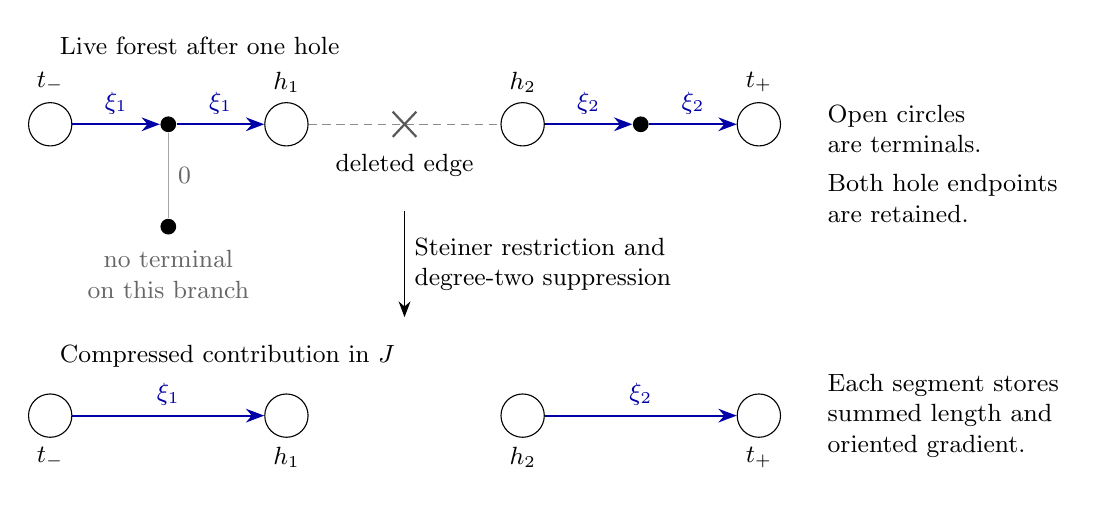
\begin{tikzpicture}[
    font=\small, >=Stealth,
    terminal/.style={circle,draw,fill=white,minimum size=5.5mm,inner sep=0pt},
    ordinary/.style={circle,fill=black,minimum size=2mm,inner sep=0pt},
    flow/.style={->,thick,blue!65!black},
    labelbox/.style={fill=white,inner sep=2pt}
  ]
    \node[anchor=west] at (0,1) {Live forest after one hole};
    \node[terminal,label=above:$t_-$] (ta) at (0,0) {};
    \node[ordinary] (va) at (1.5,0) {};
    \node[terminal,label=above:$h_1$] (ha) at (3,0) {};
    \node[terminal,label=above:$h_2$] (hb) at (6,0) {};
    \node[ordinary] (vb) at (7.5,0) {};
    \node[terminal,label=above:$t_+$] (tb) at (9,0) {};
    \draw[flow] (ta) -- node[above] {$\xi_1$} (va);
    \draw[flow] (va) -- node[above] {$\xi_1$} (ha);
    \draw[flow] (hb) -- node[above] {$\xi_2$} (vb);
    \draw[flow] (vb) -- node[above] {$\xi_2$} (tb);
    \draw[densely dashed,black!45] (ha) -- (hb);
    \draw[black!65,thick] (4.35,-.16) -- (4.65,.16);
    \draw[black!65,thick] (4.35,.16) -- (4.65,-.16);
    \node[below] at (4.5,-.25) {deleted edge};
    \node[ordinary] (leaf) at (1.5,-1.3) {};
    \draw[black!35] (va) -- node[right,text=black!60] {$0$} (leaf);
    \node[anchor=north,text=black!60,align=center] at (1.5,-1.48)
      {no terminal\\on this branch};
    \node[align=left,anchor=west,text width=3.2cm] at (9.75,-.5)
      {Open circles\\are terminals.\\[3pt]
       Both hole endpoints are retained.};

    \draw[->,semithick] (4.5,-1.1) --
      node[right,align=left,text width=4.5cm]
        {Steiner restriction and\\degree-two suppression} (4.5,-2.45);

    \node[anchor=west] at (0,-2.95) {Compressed contribution in $J$};
    \node[terminal,label=below:$t_-$] (cta) at (0,-3.7) {};
    \node[terminal,label=below:$h_1$] (cha) at (3,-3.7) {};
    \node[terminal,label=below:$h_2$] (chb) at (6,-3.7) {};
    \node[terminal,label=below:$t_+$] (ctb) at (9,-3.7) {};
    \draw[flow] (cta) -- node[above] {$\xi_1$} (cha);
    \draw[flow] (chb) -- node[above] {$\xi_2$} (ctb);
    \node[align=left,anchor=west,text width=3.2cm] at (9.75,-3.7)
      {Each segment stores summed length and oriented gradient.};
  \end{tikzpicture}
  \caption{Compression preserves a net tree flow whose divergence is
    supported on terminals. The shown targets $t_-,t_+$ and hole endpoints
    $h_1,h_2$ are retained; the terminal-free branch has zero flow, and each
    surviving path becomes one segment with the same coefficient. This is
    the tree compression used in constructing the remainder for
    Lemma~\ref{lem:backend-reduction}; the pictured contribution need not be
    closed. Vertices shown here are copied tree nodes. Physical hubs, null
    connectors, selected chords, and the contributions of every other
    frozen and raw forest join the same child graph $J$.}
  \label{fig:frozen-compression}
\end{figure}


\begin{samepage}
\begin{lemma}[One-level quality reduction]
In every state of an epoch, suppose the active logical path
assignments use selected chords and have at most $p_*$ hops.
\label{lem:backend-reduction}
Let $L_{\mathrm{best}}$ be the largest local correction score
\eqref{back:local-score}, or zero if there is none.  Then, for every
nonzero circulation $\Delta$ on the current nonloops,
\begin{equation}
\label{back:reduction-bound}
 \frac{|\gamma^{\mathsf T}\Delta|}{\|\ell\Delta\|_1}
 \le 2Z_*A_*L_{\mathrm{best}}+12Z_*A_*\OPT(J)
 \le b^2\max\{L_{\mathrm{best}},\OPT(J)\}.
\end{equation}
This conclusion is simultaneous for all current circulations and
requires no independence between the state and the verified covers
or path assignments.
\end{lemma}
\end{samepage}

\begin{proof}
Use the coefficients and raw vector of
Lemma~\ref{back:frozen-decomposition}, and form on the child edges
\begin{equation}
\label{back:child-vector}
                  \Xi_0=\sum_f\alpha_fJ_f-\widehat z_L+\Delta_n,
\end{equation}
with $\Delta_n$ carried by the hub-to-hub new edges.  Its physical
projection is
\[
                \pi\Xi_0=\Delta-\sum_f\alpha_f\pi B_f,
\]
a physical circulation.  Since $W_f\le2w_f$, the norm estimates give
\begin{align}
 \|\ell^J\Xi_0\|_1
 &\le 2Z_*A_*\|\ell\Delta_s\|_1
            +A_*\|\ell\Delta_s\|_1+\|\ell\Delta_n\|_1\notag\\
 &\le4Z_*A_*\|\ell\Delta\|_1.
                                    \label{back:child-norm-before}
\end{align}
The vector $\Xi_0$ need not balance at each compressed copy of a
physical vertex.  Route its imbalance there along the null edge to
that vertex's hub.  The hub then balances because the sum of
divergences over all copies with its physical image is zero.
The total absolute imbalance at the compressed vertices is at most
twice the sum of absolute coefficients of $\Xi_0$, and hence at
most twice its length norm, since every child edge has length at
least one.  The resulting child circulation $\Xi$ therefore satisfies
\begin{equation}
\label{back:child-norm-after}
 \pi\Xi=\pi\Xi_0,\qquad
              \|\ell^J\Xi\|_1\le12Z_*A_*\|\ell\Delta\|_1.
\end{equation}
Its gradient equals that of its projection because all connectors
have zero gradient.

For the local part, \eqref{back:local-score} and
\eqref{back:coefficient-bound} give
\[
 \left|\sum_f\alpha_f\gamma^{\mathsf T}\pi B_f\right|
 \le L_{\mathrm{best}}Z_*\sum_f|\alpha_f|W_f
 \le2Z_*A_*L_{\mathrm{best}}\|\ell\Delta\|_1.
\]
The child circulation contributes at most its norm times $\OPT(J)$,
with the same conclusion if it is zero.  Adding these inequalities
proves the first bound in \eqref{back:reduction-bound}.  The second
follows from $14Z_*A_*\le20Z_*A_*\le b^2$.

Every distribution, coupling, coefficient, and comparison vector
in this proof is existential.  The algorithm constructs only
integral graphs, terminal sets, path assignments, and rational
scores.  Once the covers and assignments have their verified
properties, the argument applies to any state and any circulation
chosen afterwards.  This proves the asserted adaptive scope.
\end{proof}

\begin{corollary}[Quality through the recursion]
\label{back:quality-induction}
Assume the path assignments and public forest lifting of
Section~\ref{sec:backend-updates}.  The backend at level $i$ returns
a certified score at least
\begin{equation}
\label{back:level-score}
                    \frac12 b^{-2(d-i)}\OPT_i.
\end{equation}
At the outer level this is at least $M^{-10/a}\OPT$.
\end{corollary}

\begin{proof}
At the bottom use Lemma~\ref{back:base}.  At a higher level compare
the local correction scores, exact current-loop scores, and the
recursive child score.  Lemma~\ref{update:flat-lift} preserves the
child gradient under lifting and does not increase raw actual length,
so the child's certified score remains valid.  If its approximation
factor is $\eta\le1$, the maximum of its score and
$L_{\mathrm{best}}$ is at least
$\eta\max\{L_{\mathrm{best}},\OPT(J)\}$.  Apply
Lemma~\ref{lem:backend-reduction} to lose at most $b^2$ at this
level.  Exact loop candidates give the same conclusion for the full
graph.  This proves \eqref{back:level-score} by induction.

Since $d=2a-4$, the outer factor is
$\tfrac12M^{-(4a-8)/a^2}$, which exceeds $M^{-10/a}$ in the checked
range.  A zero optimum does not require a positive answer.  The
representation size, explicit forest logs, and total operation cost
are established next; the quality argument itself has incurred only
one recursive child call at each level.
\end{proof}

\section{Maintaining and exposing the cycle backend}
\label{sec:backend-updates}

We now implement the reduction of Section~\ref{sec:backend-quality}.
There are two quantities to control: the work performed locally and the
number of edits passed to the one recursive child.  The latter must be
smaller, since it is multiplied through the recursion.  We also construct
the public forest, with explicit persistent edge identities, so that a
child path can be lifted without traversing all its edges.

Recursive vertex and edge sparsification for dynamic minimum-ratio
cycles is developed in \cite[Sections~5 and~7]{IncrementalGraphs}.
Here we establish the snapshot, edit-count, and forest-lifetime
guarantees required by Lemma~\ref{lem:flat-cycle}.

Retain the parameters of Section~\ref{sec:backend-quality}.  Throughout
this section a \emph{logarithmic factor} means
$\log^{O_a(1)}(2+M)$, with a constant depending on the fixed parameters
$a,\sigma$.  Different occurrences may denote different factors.  In
particular $P_*,p_*$, the number of forest copies, and the number of width
buckets are logarithmic factors.  We do not replace these factors by
powers of $b$ when accounting for work.  At recursion level $i<d$, an
epoch has $h_i=n_i/k$ single input edits.  A price replacement is a
deletion followed by an insertion.  Queries do not advance this epoch
counter.

\subsection{Class changes and immutable assignment snapshots}

Use one logical graph for each frozen tree $T^0$ and width $W$, grouping
all components of that tree in the same graph.  Thus neither rebuilding
nor taking the best score incurs a separate overhead for every component.
Let $D_T$ bound the combined tree and chord degree at a frozen tree
vertex, and set
\begin{equation}
 D_\ell=(k+1)(D_T+1)^2.
 \label{update:logical-degree}
\end{equation}
The maximum can be measured when the tree is built.  Cell-tree edges use
actual incidences; a null pair chord only joins copies of the same slot
in different partitions of one layer.  At a vertex $V_j(v)$ there are
only the appropriate OUT and IN links, and, at $V_0(v)$, the old actual
chord incidences.  Hence $D_T$ is bounded by the input degree plus
$O(K_h)$ and is a logarithmic factor whenever the input degree is.

\begin{lemma}[Class edits]
\label{update:classes}
The leg assignments of Section~\ref{sec:backend-quality} can be maintained
with logical degree at most $D_\ell$.  One input edit induces only a
logarithmic factor many logical edit units across all tree--width
graphs, where a unit is a class split, a pair of fragment-class births
at a cluster activation, or a single chord death.  Each unit involves
at most $O(D_\ell)$ incidence work.  Every change to the leg of a
surviving active incidence entails a split of its class.
\end{lemma}

\begin{proof}
Call a chord \emph{regular} when its frozen fundamental tree path meets
the initial portal grid.  The nearest-portal regions are connected:
along a shortest tree path toward the chosen portal, the distance
comparison with every competing portal persists, as does the global
index tie rule.  A region consists of its portal and parts of the
adjacent pockets, and therefore has at most $1+kD_T$ vertices.

The target of a regular incidence is the first hole on its fixed path
toward its original portal, stopped on the incidence side, or the portal
if there is no such hole.  For a fixed bucket, all current legs crossing
a newly cut edge belong to one old class.  Indeed that edge lies in one
nearest-portal region, and their earlier truncation, if present, is the
first hole on their common suffix toward the portal.  Split this class
by moving the crossing incidences to the incidence-side endpoint of the
new cut.  This target is determined by the newly cut parent edge toward
the portal, so no merging is needed.  Give \emph{both} children fresh
labels, even when one is empty or one retains the old target.

For a nonregular chord, use the two depth-band clusterings described in
Section~\ref{sec:backend-quality}.  The first interior cut activates the
cluster and creates two fresh fragment classes.  Every newly active
chord has both incidences in these new classes, including chords whose
two incidences lie on the same side.  Thereafter cuts split fragment
classes, again with fresh labels on both sides.  Classes in different
clusters remain distinct even if their targets are the same tree node.
Each cluster is contained in an initial pocket.  Its number of
incidences, and that of any regular region, is bounded by
\eqref{update:logical-degree}.  The two incidences of a logical loop are
counted separately.

An old actual-edge deletion creates only a logarithmic factor many
holes and chord deaths in all copies.  In one width bucket, a hole is
interior to at most one cluster in each of the two shifted band
partitions, and it causes at most the regular split just described.
A newly inserted physical edge creates no frozen chord.  These facts
give the asserted number of units.

Here is an explicit way to list and process them.  At freezing time,
compute tree ancestor tables, length and oriented-gradient prefix sums,
portal mark counts, nearest portals, pockets, and cluster membership.
The band index at a pocket vertex is an integer quotient of its weighted
depth; connected components of equal band index give the clusters.
No record is allocated for an empty band.  These computations take
near-linear tree work up to logarithmic factors and determine the
relevant path sums without scanning each fundamental path.  Initial
regular legs have at most $k+1$ tree edges, so their membership lists on
tree edges can also be built explicitly.  On a hole, inspect the
region-bounded lists, discard dead incidences and legs already stopped
before this hole, and update the remaining class lists.  A cluster cut
can inspect the whole small cluster and its chord incidences.

Before activation, keep each direct fundamental-cycle score in a heap
using its frozen sums.  Delete its entry when the chord dies or its
cluster activates.  For an input death, physical chord removals can be
processed before the splits and activations that it causes.  Afterwards
every surviving active leg is the unique live tree path to its stored
target.  A leg whose class has not split retains that path and its
gradient.  This also proves the last assertion.
\end{proof}

We maintain assignments by an inner hierarchy of snapshots.  At edit
$h_i$ rebuild the whole outer epoch on the resulting input graph,
without updating the obsolete child.  For edits $1\le t<h_i$, put
\begin{equation}
 z_0=\lceil\log_b h_i\rceil\le a^2,
 \qquad s_j=b^{z_0-j}\quad(0\le j\le z_0).
 \label{update:periods}
\end{equation}
These are integral powers of two under the divisibility assumption on
$u$.  Level zero is the initial frozen assignment.  At tick $t$, choose
the smallest $j\ge1$ for which $s_j\mid t$.  Rebuild from the parent
snapshot at
\begin{equation}
 t_0=\left\lfloor\frac{t}{s_{j-1}}\right\rfloor s_{j-1}<t,
 \qquad t-t_0\le b s_j,
 \label{update:parent-time}
\end{equation}
and let all finer levels share the resulting snapshot.  Minimality of
$j$ ensures $s_{j-1}\nmid t$, so the strict inequality in
\eqref{update:parent-time} holds.  If a coarser level was rebuilt at
$t_0$, its shared snapshot also supplies the indicated parent.

An assigned path is simple; an empty path visits its sole vertex once.
The invariants for a level-$j$ snapshot are
\begin{equation}
 p(j)=(10P_*)^{j+1},\qquad
 C(j)=D_\ell(100P_*)^{j+1},
 \label{update:snapshot-bounds}
\end{equation}
bounding its path hops and the number of assigned paths visiting any
one class, respectively.  At initialization only regular chords are
active and their classes are portals.  Apply
Lemma~\ref{lem:routing-helper} with endpoint incidence counts as
resources and simplify the returned walks.  For nonempty walks,
vertex visits are bounded by endpoint incidence charges on their
traversed edges; empty paths add at most the demand degree.  This proves
\eqref{update:snapshot-bounds} for $j=0$.  All finer levels initially
share this snapshot.

Selections are physical chord identifiers.  A selected chord remains
in support for the rest of the epoch while alive, even if its logical
endpoint classes later split.  Repeated selection stores it just once
in the child graph.

\begin{lemma}[The anchor core]
\label{update:anchor-core}
Suppose the interval from a parent snapshot to a rebuild contains
$E_0$ logical edit units in one tree--width graph.  The rebuild can
restore \eqref{update:snapshot-bounds} using a helper instance on
$O(E_0)$ incident labels.  It selects at most $O(P_*E_0)$ additional
central chords.  The work is
\begin{equation}
 O(1+D_\ell E_0)\,bM^{o_a(1)},
 \label{update:rebuild-work}
\end{equation}
in addition to scanning the interval's edit log with logarithmic
overhead per tick and explicitly handled incidence.
\end{lemma}

\begin{proof}
Mark labels of the snapshot at $t_0$ as follows.  Every split marks its
ancestor at $t_0$, if one exists; every chord death marks the ancestors
of both endpoint classes.  Let $Y$ be the marked set.  Then
$|Y|\le2E_0$.  The \emph{anchors} are all current descendants of $Y$
and all current classes born from activations after $t_0$, including
their later descendants.  There are $O(E_0)$ anchors: initially marked
labels contribute at most $2E_0$, and every subsequent split or
activation adds only constantly many class labels.  Ancestors absent
at $t_0$ belong to the latter activation families.

Mark every old assigned path that visits $Y$, including at an endpoint.
In particular the path of a deleted demand is marked, as is any path
using a deleted support edge.  Every unmarked path still uses the same
live oriented chords on unchanged labels.  Moreover its demand and
all support edges on the path retain the same legs and leg gradients,
by Lemma~\ref{update:classes}.  Thus its correction
$B_f=L_f-L_{\Pi_f}$ has exactly the stored gradient.  A hole outside
these legs can change the clipped comparison vector, but does not
change this correction.  Inactive direct-cycle candidates are handled
separately by their activation lists.

Consider a marked old path whose demand $e$ survives.  Follow its
prefix from the tail to the first marked label.  Every preceding label
is unsplit.  Every edge of this prefix is live: if one had died, its
earlier endpoint's old label would also have been marked.  The final
edge now ends at a current descendant of the first marked label.
Interpreting the same oriented edges therefore gives a current path
$A_e$ from the current tail to an anchor.  If the old path starts
marked, $A_e$ is the empty path at the current tail.  Reversing this
argument gives a suffix $Z_e$ from a current anchor to the current head
at the last marked label.  Repeated splits cause no ambiguity, since
the current incidence of the last prefix edge specifies its current
descendant.  For newly activated demands use empty $A_e,Z_e$; both
endpoints are anchors by the activation rule.

For each such demand put an edge in a core graph on the anchors,
associated with the direct logical walk
\begin{equation}
                 -A_e+e-Z_e.
 \label{update:core-walk}
\end{equation}
Its orientation is from the end of $A_e$ to the beginning of $Z_e$;
a minus reverses a path.  For every current base class use its number
of visits on this direct walk as a resource count.  Each count is at
most two.  Indeed the prefix and suffix each come from a simple old
path, with at most their final marked label replaced by a descendant;
the two resulting vertex lists concatenate across $e$.  This also
covers empty prefixes, suffixes, and a loop demand.  The total resource
count at a class, over all direct walks, is at most
\begin{equation}
                  C_0=2C(j-1)+D_\ell.
 \label{update:core-resource}
\end{equation}
Prefix visits and suffix visits of old demands charge separately to
visits at that class's old ancestor; newly activated endpoint
incidences charge to its current degree.  The same bound controls
the core demand degree, because its endpoint incidences are among
these resource visits.

Apply Lemma~\ref{lem:routing-helper} to the core with the resources
just defined.  Lift its assigned walks by substituting
\eqref{update:core-walk}, and for demand $e$ prepend $A_e$ and append
$Z_e$.  Simplify the resulting walk to a simple path, erasing the whole
walk if its endpoints coincide.  Cycle erasure never increases hops
or resource visits.  The hop count before simplification is at most
\begin{equation}
 2p(j-1)+P_*\bigl(2p(j-1)+1\bigr)\le p(j).
 \label{update:hop-induction}
\end{equation}
The substituted helper walks cost at most $P_*C_0$ visits at each
class.  The added prefixes and suffixes cost at most
$2C(j-1)+D_\ell$, including the empty paths; the unchanged assignments
add at most $C(j-1)$.  Thus a valid upper bound is
\[
 P_*\bigl(2C(j-1)+D_\ell\bigr)+3C(j-1)+D_\ell
 \le100P_*C(j-1)=C(j).
\]
All edges in the prefixes and suffixes were already live support
edges.  Only the central chords of the selected core edges must be
added to support.  The core has $O(E_0)$ incident labels, regardless
of how many old paths met $Y$, so the helper selects at most
$O(P_*E_0)$ such chords.  When $E_0=0$ the old snapshot can simply be
retained.

For completeness, the implementation does not copy whole snapshots.
Each held snapshot consists of immutable balanced-dictionary roots
for paths keyed by demand, an index from class to its visiting paths,
and an ordered collection of correction-score keys.  Path copying
changes only the search paths of modified dictionary entries.  Begin
with the parent roots and replace marked or dead records and add the
newly active records.  The class index enumerates at most
$C(j-1)|Y|$ old path occurrences before their lists are read; a
dictionary removes duplicates.  Activation lists enumerate new
demands.  Every such path has logarithmic-factor length, and the
number of newly activated demands is at most $O(D_\ell E_0)$.

Store split-parent pointers with class birth ticks and jump pointers.
To find the ancestor at $t_0$, follow this history to the class alive
at the end of tick $t_0$.  All splits within one tick belong to that
tick and snapshots are taken only after settlement, so equal birth
ticks do not create a partially settled ancestor.  Physical chord
identifiers, the two current incidence classes, and their targets
are explicit records.  They determine the oriented lifted prefixes
and suffixes.  Frozen tree prefix data gives each live leg's gradient
and length; summing over the new short logical paths recomputes their
correction-score keys.  Unmodified keys remain valid by the unmarked
path argument.

Building the direct lists and the helper's resource lists, simplifying
its output, and changing the indices costs
$O(1+D_\ell E_0)bM^{o_a(1)}$ by
Lemma~\ref{lem:routing-helper}.  Comparing the maintained best keys
over the logarithmic-factor many tree--width graphs has only
logarithmic overhead.  The helper's input prerequisites can be checked:
twice the demand count and the nonzero resource-list length must each
be at most $M^2$.  They hold for all sufficiently large $M$ at fixed
parameters, since even all frozen chords number at most
$O(n_i)$ times a logarithmic factor, and every direct walk has
logarithmic-factor length.  This proves the work assertion and both
snapshot invariants.
\end{proof}

\begin{lemma}[Cumulative assignment work and support]
\label{update:support}
The initial assignments use at most $h_i$ times a logarithmic factor
many support chords.  On every epoch prefix of $t'\le h_i$ edits, the
additional support selections number at most $bt'$ times a logarithmic
factor, and local assignment work is
$t'M^{O(1/a)+o_a(1)}$ after initialization.  Initialization costs
$n_iM^{O(1/a)+o_a(1)}$.
\end{lemma}

\begin{proof}
Initially the number of portal classes, summed over all tree--width
graphs, is at most $(n_i/k)$ times a logarithmic factor.  The helper
selects at most $P_*$ times this many chords.  At inner level $j$ there
are at most $\lfloor t'/s_j\rfloor$ rebuilds, each using an interval
of at most $bs_j$ ticks.  By Lemma~\ref{update:classes}, the sum of
their interval edit counts across all tree--width graphs is at most
$bs_j$ times a logarithmic factor per rebuild.  Consequently the
cumulative support additions at that level are at most $bt'$ times
a logarithmic factor by Lemma~\ref{update:anchor-core}.  There are at
most $a^2$ inner levels.  Summing
\eqref{update:rebuild-work} similarly bounds the local work by
$t'D_\ell b^2$ times a logarithmic factor, in addition to smaller
constant-per-rebuild and log-scanning costs.  Since
$D_\ell=(k+1)\log^{O_a(1)}(2+M)$, this has the asserted exponent with
an absolute coefficient.  Initial tree preparation, the explicit
short regular-leg lists, and initial helper calls fit the stated
initialization bound.  A physical removal lists the deaths of selected
copies in logarithmic-factor work.  Keeping earlier live selections
therefore requires no additional support budget.
\end{proof}

In particular \eqref{update:hop-induction} gives
$p(j)\le(10P_*)^{a^2+1}=p_*$, supplying the path assumption in
Lemma~\ref{lem:backend-reduction}.

\subsection{Small changes to the compressed child}

The snapshot hierarchy now supplies the short selected-support paths
required by the quality reduction.  We next bound the number of edits
needed to maintain their compressed representation in the child graph.
Afterwards, the public forest construction will expose child paths
while preserving the identities of retained mapped edges.

\begin{lemma}[Compressed graph edits]
\label{update:compressed-edits}
The single child graph $J$ can be initialized nonempty.  Throughout
an epoch it uses at most $h_ib$ times a logarithmic factor many active
slots and edges, including slots assigned earlier in that epoch.
On an epoch prefix of $t'$ further input edits it receives at most
$bt'$ times a logarithmic factor individual edits.  Its degree is a
logarithmic factor, and its integral prices obey the level-$(i+1)$
bounds.  The local construction work per parent edit is
$M^{O(1/a)+o_a(1)}$ amortized.
\end{lemma}

\begin{proof}
Initial terminal promotions number at most $h_i$ times a logarithmic
factor.  Subsequent promotions come from hole endpoints, new class
targets, endpoints of selected support chords, and the raw-hierarchy
route endpoints needed for new physical incidences.  The first three
counts follow from Lemmas~\ref{update:classes} and
\ref{update:support}.  For the fourth, enumerate the
$K_h^{O(r)}$ possible sequences of partition options from the given
physical slot.  At each step look up the entering copy and its frozen
cell root in stored tables.  This lists the needed endpoints without
traversing the raw legs.  It costs a logarithmic factor per incidence.
Thus the cumulative additional promotions on a prefix number at most
$bt'$ times a logarithmic factor.  Retain all promoted terminals until
the epoch ends.

Build each initial Steiner subtree in bulk, using subtree terminal
counts.  To promote one additional tree node, split its current
compressed segment if it is already in the represented subtree.  If
it is outside, explore its hanging component to the unique attachment
and add the joining path, splitting the segment at that attachment if
needed.  If the live component has no represented subtree, create an
isolated terminal.  The explored exterior component contains no
initial portal, and hence lies within one original pocket of fewer
than $k$ vertices.  Existing segments have at most $k+1$ constituent
edges.  Membership and segment pointers on these nodes, together with
local forest adjacency, therefore suffice for
$O(k+1)$ times degree and logarithmic-factor work.  Only $O(1)$
compressed vertices and edges change per promotion.  No whole live
component must be relabeled.

Before cutting a frozen tree edge, promote both endpoints.  The edge
is now itself a compressed segment and can be deleted.  On either
side, every other represented edge still separates terminals: a
terminal formerly reached across the deleted edge is replaced for
this purpose by its now-terminal endpoint.  Thus there is no pruning
or merging cascade.  Keep each segment's full constituent list with
orientations.  A changed segment or changed realization is removed
and replaced by a fresh edge, with deletion first.

Assign each represented frozen tree or raw-forest node its own child
slot, without reuse in this invocation, and assign at most one hub
per physical label.  A selected chord remains attached at its
original tree-node endpoints.  Its logical leg targets can therefore
change in bulk without migrating its child edge.  New actual
nonloops are inserted directly between hubs and removed at their
deaths; actual loops have already been handled by the loop heap.
These rules establish the claimed size and edit counts.

Reserve $\lfloor n_{i+1}/2\rfloor$ child slots, with unused slots
isolated, and check both assignment overflow and total slots plus
current edges against the child's capacity.  For fixed parameters
these checks hold eventually, because
\begin{equation}
 n_{i+1}=h_iM^{1/(2a)},\qquad
 b=M^{1/a^2},\qquad \frac1{a^2}<\frac1{2a}.
 \label{update:child-slack}
\end{equation}
The active-slot and edge bounds above are consequently smaller than
either reserved half for all sufficiently large $M$.

At a compressed node, segment degree is at most its frozen tree
degree; add its chord degree and one hub connector.  At a hub, the
connector degree is bounded by the number of frozen tree and
raw-forest copies of its physical label, plus the current new actual
incidences.  Both are logarithmic factors.  Deleting old segments
before adding replacements preserves these degree bounds even
during the child edit sequence.  This proves the degree hypothesis
inductively from the degree-three outer input.

A segment sums prices over at most $k+1$ edges, so its positive
integral length and absolute gradient are at most
$(k+1)M^{G_i}\le M^{G_i+2}=M^{G_{i+1}}$ for adequate parameters.
Other child prices are inherited or are $(\ell,\gamma)=(1,0)$.
The local work includes an $O(k+1)$ factor per promotion or changed
segment and the assignment work already bounded.  Its exponent is
therefore $O(1/a)$ with an absolute coefficient.  Only the smaller
\emph{edit count} proved above is passed into the recursive time
bound.
\end{proof}

\subsection{A public forest with prebuilt arms}

This representation uses the flat-embedding viewpoint of
\cite[Definition~2.3 and Theorem~3.5]{IncrementalGraphs}, whose
minimum-ratio-cycle data structure is fully dynamic.
The preallocation and reassignment of unused tree copies follow the
flat-forest lifting construction of Kyng, Meierhans, and Probst Gutenberg
\cite[Section~3.3, Lemma~3.21 and Algorithm~5]
{KyngMeierhansProbstGutenberg2023FlatForest}.  Their construction already
provides path-length domination and bounds on changes to the lifted
forest.  Here the copied trees are the arms of compressed segments.
We track the lifetime of every mapped edge and process each parent edit
as one old-to-final transaction; these details preserve the engine's
signed and absolute accumulations when an unused copy is reassigned.

Put
\begin{equation}
                D_i=b^{2(d-i)}\qquad(0\le i\le d).
 \label{update:occurrence-bounds}
\end{equation}
The bottom forest is empty.  At a higher level include full live
copies of all $T^0$ and raw $H_j$ forests as separate public
components, with their holes and their actual or null mappings.
They represent local correction paths and individual compressed
segments.  The following additional components, disjoint from the
full copies, represent the recursively exposed forest $F^J$.

For each active child slot $q$, including hubs, write $\varphi(q)$
for its physical image.  Prebuild a pool of $D_{i+1}$ \emph{arm slots}.
An arm slot has a center mapping to $\varphi(q)$.  For each tree
segment of $J$ incident to $q$, attach an independent copy of its
entire constituent path, oriented outward from $q$, with a fresh far
tip and all constituent vertex and edge maps.  Different arms in
one slot meet only at its center; different slots are disjoint.
Retain the whole pool, including unassigned, or \emph{dormant}, slots.
Assign a distinct arm slot to each occurrence of $q$ in $F^J$.
Occurrences over an inactive child slot are ignored publicly: such
a slot is isolated in $J$, so all its forest components have only
null edges and project to that one slot.

Add one connector for every child forest edge in the active part:
\begin{enumerate}
\item If its map is a segment $qz$, choose a fixed endpoint side,
say $q$.  Use the corresponding arm in the slot assigned to its
occurrence over $q$, and add a null connector from that arm's far
tip to the center assigned to the other occurrence over $z$.
\item If its map is a nonsegment child edge, join the two assigned
centers with that edge's single actual-edge or null map.
\item If the child forest edge itself is null, join its assigned
centers with a null connector.
\end{enumerate}
The endpoints of each null connector have equal physical images.
Centers have indexed identifiers, and tips are indexed by arm slot
and incident segment identifier.  Connector endpoints can thus be
looked up without scanning an arm.

\begin{lemma}[Flat lifting]
The construction is a forest with valid current actual or null edge
maps.  \label{update:flat-lift}
A child forest-path piece lifts to at most one public forest-path
piece, preserving its signed projection and with parent raw length
at most its child raw length.  An individual child-edge piece lifts
to one path or one actual-edge piece, or can be omitted if null.
The lifted sum of a child circulation is a circulation with the same
gradient.  The number of returned pieces is
$M^{O(1/a)+o_a(1)}$.
\end{lemma}

\begin{proof}
Contract every arm-slot tree to its center.  On assigned slots the
connector quotient is exactly the active subforest of $F^J$.
Dormant slots have no connectors.  A cycle in the expanded graph
would give a cycle in this quotient, since each contracted part is
itself a tree.  Together with the disjoint full copies, the result
is a forest.

Expand each edge on an oriented child path using the prescribed
arm and connector, or its nonsegment connector.  The concatenation
has the expanded signed projection of that child path.  Segment
length is the sum of its constituent parent lengths; null child
edges contribute zero parent raw length, and other child null
realizations can only decrease it.  Thus the concatenation's
parent raw length is at most the sum of child-edge lengths counted
with their traversal multiplicities.

This concatenation may backtrack, even when the child path is
simple, because several connectors can use the same arm in one
slot.  In a forest, deleting a consecutive edge and its reverse
preserves the signed count of every oriented edge and decreases
nonnegative raw length.  Repeating this deletion leaves the unique
forest path between the assigned endpoint centers.  It therefore
has exactly the needed projection and no larger raw length.  We
return its endpoints; we do not perform these cancellations by
expanding the walk.  If the child path has an inactive endpoint,
its whole component is one of the ignored null components, so the
piece can be omitted.

For a piece given as a single child segment, use its endpoints in
the appropriate full live forest copy.  For a nonsegment piece,
return its actual edge or omit its null realization.  Each edge
expansion has divergence equal to its mapped endpoint divergence.
Summing a child circulation therefore gives zero physical
divergence and preserves its gradient.  In particular a positive
child score gives positive gradient magnitude after lifting and
therefore positive parent raw length.  Its score remains a valid
lower bound for the lifted ratio.

Only endpoint and slot lookups are needed in these conversions;
no long lifted path is traversed or priced anew.  A local correction
uses $O(p_*)$ pieces in full copies and individual actual chords,
with opposite traversals explicitly reversed and null chords
omitted.  An actual loop uses one piece.  A child answer gives at
most as many parent pieces as it had child pieces.  At each level
we return one best candidate, rather than concatenating candidates
from several levels.  The bottom answer has at most
$n_d=M^{2/a}$ pieces.  Taking the maximum of these bounds proves the
last assertion.  Every listed piece has unit multiplicity;
repetitions, if present, are listed and charged.
\end{proof}

Figure~\ref{fig:arm-slots} shows the shared-arm lift and a dormant slot
whose internal edge lifetimes persist through reassignment.
\begin{figure}[!htbp]
  \centering
  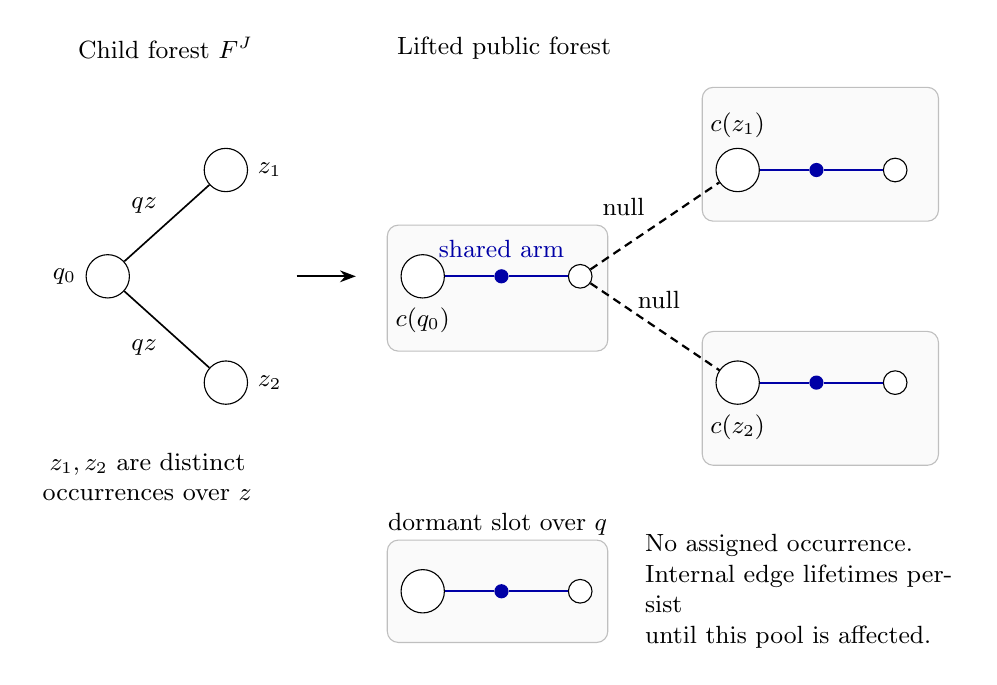
\begin{tikzpicture}[
    font=\small, >=Stealth,
    center/.style={circle,draw,fill=white,minimum size=5.5mm,inner sep=0pt},
    tip/.style={circle,draw,fill=white,minimum size=3mm,inner sep=0pt},
    mid/.style={circle,fill=blue!65!black,minimum size=1.8mm,inner sep=0pt},
    arm/.style={thick,blue!65!black},
    connector/.style={thick,densely dashed},
    slot/.style={draw=black!25,fill=black!2,rounded corners=4pt}
  ]
    \node[anchor=west] at (0,2.9) {Child forest $F^J$};
    \node[center,label=left:$q_0$] (q) at (.5,0) {};
    \node[center,label=right:$z_1$] (z1) at (2,1.35) {};
    \node[center,label=right:$z_2$] (z2) at (2,-1.35) {};
    \draw[semithick] (q) -- node[above left] {$qz$} (z1);
    \draw[semithick] (q) -- node[below left] {$qz$} (z2);
    \node[align=center,text width=2.8cm] at (1,-2.55)
      {$z_1,z_2$ are distinct\\occurrences over $z$};
    \draw[->,semithick] (2.9,0) -- (3.65,0);

    \node[anchor=west] at (4.05,2.9) {Lifted public forest};
    \draw[slot] (4.05,-.95) rectangle (6.85,.65);
    \draw[slot] (8.05,.7) rectangle (11.05,2.4);
    \draw[slot] (8.05,-2.4) rectangle (11.05,-.7);
    \node[center,label=below:$c(q_0)$] (cq) at (4.5,0) {};
    \node[mid] (mq) at (5.5,0) {};
    \node[tip] (tq) at (6.5,0) {};
    \draw[arm] (cq) -- (mq) -- (tq);
    \node[above,text=blue!65!black] at (5.5,.12) {shared arm};
    \node[center,label=above:$c(z_1)$] (cz1) at (8.5,1.35) {};
    \node[mid] (mz1) at (9.5,1.35) {};
    \node[tip] (tz1) at (10.5,1.35) {};
    \node[center,label=below:$c(z_2)$] (cz2) at (8.5,-1.35) {};
    \node[mid] (mz2) at (9.5,-1.35) {};
    \node[tip] (tz2) at (10.5,-1.35) {};
    \draw[arm] (cz1) -- (mz1) -- (tz1);
    \draw[arm] (cz2) -- (mz2) -- (tz2);
    \draw[connector] (tq) -- node[above left] {null} (cz1);
    \draw[connector] (tq) -- (cz2);
    \node[fill=white,inner sep=1pt] at (7.5,-.3) {null};
    \draw[slot] (4.05,-4.65) rectangle (6.85,-3.35);
    \node[center] (cd) at (4.5,-4) {};
    \node[mid] (md) at (5.5,-4) {};
    \node[tip] (td) at (6.5,-4) {};
    \draw[arm] (cd) -- (md) -- (td);
    \node[above] at (5.45,-3.42) {dormant slot over $q$};
    \node[anchor=west,align=left,text width=4cm] at (7.2,-4)
      {No assigned occurrence.\\
       Internal edge lifetimes persist\\
       until this pool is affected.};
  \end{tikzpicture}
  \caption{A shared-arm lift in Lemma~\ref{update:flat-lift}. Both child
    edges map to the same segment $qz$, but their endpoint occurrences over
    $z$ use different slot trees. Each edge adds one null connector from
    the far tip of the chosen arm to the other assigned center.
    Contracting all slot trees recovers the child forest. In the child path
    from $z_1$ to $z_2$, the two traversals of the shared arm cancel when
    the concatenated realization is reduced to the unique forest path;
    signed projection is preserved and raw length cannot increase.
    Dormant slots retain their internal edges, so reassignment at an
    unaffected label changes assignments and connectors without rebuilding
    those edges.}
  \label{fig:arm-slots}
\end{figure}

\clearpage

\begin{lemma}[Occurrence multiplicity]
\label{update:multiplicity}
For all sufficiently large $M$ at fixed parameters, level $i$
has at most $D_i$ public forest vertices over each input slot.
In particular the outer multiplicity is at most $M^{10/a}/4$.
\end{lemma}

\begin{proof}
Full copies contribute a logarithmic factor.  For one compressed
frozen forest, segment interiors are disjoint.  Thus a node in
such an interior occurs in at most two arms per pool index, one
from each endpoint of its segment.  At a compressed endpoint,
its own centers and the far tips of arms from adjacent endpoints
contribute at most one plus its tree degree per pool index.
These bounds include dormant slots.  A physical input label has
only a logarithmic factor many frozen-tree and raw-forest copies,
and at most one hub.  Consequently its total multiplicity is
at most
\begin{equation}
       (1+D_{i+1})\log^{O_a(1)}(2+M).
 \label{update:multiplicity-step}
\end{equation}
There is no factor of the segment length in this bound.  The
$b^2$ gap between $D_i$ and $D_{i+1}$ absorbs the logarithmic
factor for sufficiently large $M$.  Induction starts with the
empty bottom forest.  Finally
\[
 D_0=M^{(4a-8)/a^2}\le M^{10/a}/4
\]
eventually.  Both the inductive multiplicities and the last
inequality may be checked as deterministic prerequisites.
\end{proof}

\subsection{Explicit recourse and persistent edge lifetimes}

An occurrence or forest edge has an immutable lifetime identifier.
Changing an occurrence's label, an edge's endpoints, or its map
requires a replacement with a fresh identifier.  A vertex death
explicitly logs all incident edge removals first.  Additions use
present endpoints.  The client retains old input labels, prices,
and maps until all old public removals have been processed, then
installs the new input state and public additions.  No path call
occurs inside this transaction.  A whole epoch boundary can remove
the old public forest and install the new one with these rules.

\begin{lemma}[Forest recourse]
\label{update:recourse}
For one parent input edit within an epoch, let $Q$ be the set of
child labels assigned or changed, or incident to a changed child
edge or changed segment realization.  Apart from local full-copy
edits, the public forest can be updated in
\begin{equation}
 |Q|D_{i+1}(k+1)\log^{O_a(1)}(2+M)
       +\mathcal L\log^{O_a(1)}(2+M)
 \label{update:recourse-cost}
\end{equation}
work and public log records, where $\mathcal L$ is the number of
child log records processed.  Retained arm edges at labels outside
$Q$ keep their lifetimes and maps, even if their arm slot is
reassigned to a different child occurrence.
\end{lemma}

\begin{proof}
First compute the batch of individual $J$ edits for this parent
operation, without a child query, and determine $Q$.  Its size is
bounded by a constant times the exogenous child edit and
assignment counts of Lemma~\ref{update:compressed-edits}.  Retain
access to the old occurrence assignments and old child forest
records.  Run the child edit sequence while maintaining a
\emph{passive} copy of its logs, indexed by lifetime identifier and
label, with individual incidence lists.  Track which records were
added or removed.  Each log changes only its own dictionary and
incidence-list entries and costs logarithmic overhead.  In
particular deleting an occurrence does not trigger an uncharged
degree scan: its incident edge deletions have their own records.
Persistent roots or saved old records retain the old information
until the parent transaction is complete.

At labels in $Q$, remove all old arm pools and construct the final
active pools with final occurrence assignments.  Sweep their old
and final incident child edges as well, to remove and reconstruct
the corresponding connectors.  To bound these sweeps, fix a label
$q$ in either the old or the final state and let $N_J(q)$ be its
set of \emph{distinct} other neighbors.  Every child forest edge
incident to an occurrence over $q$ belongs to the forest induced
on the occurrence sets over $\{q\}\cup N_J(q)$.  That forest has
at most
\begin{equation}
 D_{i+1}\bigl(1+|N_J(q)|\bigr)
       \le D_{i+1}\bigl(1+\deg_J(q)\bigr)
 \label{update:incident-forest-count}
\end{equation}
vertices, and hence no more than this many edges.  Parallel
child-graph edges only increase the safe degree bound.  A
child-null edge has both ends over $q$ and is already included.
This proves the bound separately for the old and final sweeps;
old lists can be saved before applying the child batch.
Constructing each arm takes at most $k+1$ constituent steps.
The degree bound on $J$ now gives the first term of
\eqref{update:recourse-cost}.

At every unaffected active label, retain the arm pools and the
assignments of retained occurrences.  First free assignments of
deleted old occurrences, then assign each final new occurrence
from a free-slot stack.  There is sufficient space because the
final occurrence count is at most $D_{i+1}$.  Remove the old
connectors for changed child edge records and add the necessary
final ones; also handle the connectors found in the affected
sweeps.  Additions can wait until all final assignments exist.
Deduplicate swept records by identifier.  Transient child records
that are neither old nor final need not be published by the parent,
although their individual processing is charged.

If a child edge and both its assignments survive unchanged at
unaffected labels, its connector retains the same map.  Every
other change at these labels has an explicit child edge record:
an occurrence replacement logs its incident edge removals and
new edges, and an edge endpoint or map change is itself a
replacement.  Thus the remaining work is logarithmic per child
record, giving the second term in
\eqref{update:recourse-cost}.  A high-degree child occurrence
can have many incident records, but each is processed once; it
does not add a degree sweep to each record.  Child lists over
inactive slots are likewise kept passively until activation,
which places their label in $Q$.

Full-copy hole edits are performed separately.  Every public map
to a dying parent input edge is removed: it lies in a full copy
that receives the cut, in an arm of a changed or removed segment
whose endpoints are in $Q$, or in a connector realizing a removed
nonsegment child edge.  Remove connectors before their old pool
vertices, and all old edges before their vertex deaths.  After
these removals the retained public graph is a subforest of the
final graph, so its final pools, vertices, and connectors can be
inserted in a valid order.

During this computation the child sees only its abstract slots,
edges, and integral prices.  An intermediate child state may
still contain the old realization of a parent segment whose
physical edge is about to die.  Its abstract graph remains an
in-range input, and it never asks for parent physical data.
Only the final child state must be the reduction of the new
parent input.  The parent therefore publishes one old-to-final
transaction, using retained old data for all removals, rather
than a lifted public state for every intermediate child edit.

Finally, a dormant arm slot at an unaffected label retains all
its internal edges when assigned to another occurrence.  Their
identity is determined by the child label, pool index, and
incident segment realization, not by the assigned occurrence
identifier.  Existing signed and absolute accumulations in the
client's path tracker consequently remain attached to the same
mapped edges.  No $D_{i+1}$ or $k$ factor multiplies the processing
of general child-internal occurrence changes.
\end{proof}

The two marking rules used above serve different purposes.  A
terminal promotion or segment subdivision may merely reencode
an unchanged physical path, so its logical correction need not
be marked in Lemma~\ref{update:anchor-core}.  It nevertheless
marks the endpoint arm pools in Lemma~\ref{update:recourse}.
Conversely, a logical class split changes its leg data while
selected central chords remain attached at their original tree
nodes.  This is why the logical snapshot update and public
forest update have the stated separate bounds.

\subsection{Total work, finite arithmetic, and reliability}

The recurrence must charge local arm-pool reconstruction separately
from processing the child's forest logs.  A changed child label can
require rebuilding its arms, whereas each general child log record
incurs only logarithmic overhead.  Keeping these charges separate
allows the small child edit count to control the recursive cost.

\begin{lemma}[Recursive work bounds]
\label{update:recurrences}
For a prefix of $s$ graph operations, counting queries and edits
and including an operation that terminates partway through,
level $i$ has total work and explicit public-log size at most
$n_iA_i+sU_i$, where
\[
                  A_i,U_i=M^{O(1/a)+o_a(1)}.
\]
All coefficients in the $O(1/a)$ exponents are absolute.
\end{lemma}

\begin{proof}
Give the child its arbitrary nonempty initial graph directly.
The parent's own initialization costs
$n_iM^{O(1/a)+o_a(1)}$.  This includes tree preparation, initial
assignments and compression, full forest copies, and initial
arm pools.  Initially there are only $h_i$ times a logarithmic
factor many active child labels; each has $D_{i+1}$ pools and
arms of at most $k+1$ steps.  Since $D_{i+1}\le M^{4/a}$, this
cost has the required absolute exponent.  Epoch teardown and its
public logs obey the same allowance.  Allocations and eventual
deallocation are charged; a discarded arena can be reclaimed
against its earlier allocations.

By Lemmas~\ref{update:support}, \ref{update:compressed-edits},
and \ref{update:recourse}, all local incremental work costs
$M^{O(1/a)+o_a(1)}$ amortized per input operation.  In particular
the cumulative affected-label count in an epoch prefix is only
$b$ times a logarithmic factor per parent edit.  Queries use
the maintained best keys and lift one answer, with logarithmic
overhead per child piece.  They need not alter the public forest.

Let $L=M^{C/a+o_a(1)}$, for an absolute constant $C$, dominate
these local factors and the bottom-level costs.  Such an absolute
$C$ exists: all nonlogarithmic local factors above are fixed
powers of $b$, $k$, and $D_{i+1}$; at the bottom the elementary
negative-cycle computation is a fixed-degree polynomial in
$n_d=M^{2/a}$.  Factors involving $r,a^2,P_*,p_*$ and degree
bounds are fixed-parameter logarithmic factors.

Initialization of the child contributes $n_{i+1}A_{i+1}$,
with logarithmic overhead on its logs, and
$n_{i+1}/n_i=M^{-1/(2a)}$.  At most $1+s/h_i$ parent epochs
start.  After initialization the child receives at most
$bM^{o_a(1)}$ times the parent operation count, including the
one recursive query used for a parent query.  Only a
logarithmic factor multiplies child log-processing work, by
Lemma~\ref{update:recourse}.  Consequently it suffices to choose
dominating upper estimates satisfying
\begin{align}
 A_i&=L+M^{-1/(2a)+o_a(1)}A_{i+1},\\
 U_i&=L+kA_i+M^{1/a^2+o_a(1)}U_{i+1},
 \label{update:time-recurrences}
\end{align}
with $A_d,U_d\le L$.  The term $kA_i$ pays rebuilding every
$h_i=n_i/k$ edits, including its child initialization.

For fixed $a$, the multiplier in the first recurrence tends to
zero, so $A_i\le2L$ eventually after enlarging $L$ if necessary.
Unrolling the second recurrence through at most $d\le2a$ levels
gives
\[
 U_i\le (d+1)(L+2kL)
       M^{d/a^2+o_a(1)}
       =M^{(C+3)/a+o_a(1)}.
\]
This explicitly shows why no coefficient depending on $a$
appears in the $1/a$ exponent.  Logarithmic overhead accumulated
over the fixed number of levels remains $M^{o_a(1)}$.

Each attempted cover or helper reconstruction has its own
every-path bound, whether it succeeds or is rejected.  Charge
such a reconstruction to the attempted operation, including if
failure or a guard stops it before publication.  All previously
published states satisfy their verified bounds.  The same
recurrences therefore hold for these prefixes and unsuccessful
computations.
\end{proof}

\paragraph{Finite arithmetic.}
\label{update:arithmetic}
All maintained data are finite integers, dyadics, explicit lists,
or identifiers.  Frozen tree prefix sums and segment sums use
at most the number of constituent edges times the level price
bound.  Width buckets are integer powers of two.  Correction
scores compare ratios of integral gradient magnitudes to the
positive integral proxies $Z_*W_f$ by cross multiplication;
bottom scores and inherited scores are likewise represented by
bounded integral numerator--denominator pairs.  The construction
requires no evaluation of the conceptual hierarchy-law
probabilities, real flows in the comparison argument, or
barrier logarithms.  Exact geometric delays, dyadic thresholds,
and helper randomness are generated by the finite procedures
already specified.  Fixed-parameter data have
$\log^{O_a(1)} S$ bit length, and ordinary dictionary and forest
record operations have multiword logarithmic-factor overhead.
The integral-flow calls inside the helper use the simulation of
Lemma~\ref{lem:capacity-scaling}; its logical addresses are not
assumed polynomially bounded in their numerical values.

\begin{lemma}[Guards and conditional failure]
\label{update:reliability}
The construction can enforce all size, multiplicity, arithmetic,
and sampling prerequisites by finite checks.  For every sufficiently
large fixed $a$ and every fixed $\sigma\ge0$, those deterministic prerequisites
are adequate for all sufficiently large sizes in the permitted
engine range, on every random path.  Conditional on any adaptively
specified history before an invocation, the detected sampling
failure probability over an entire engine instance is at most
$2^{-\sigma}S^{-60}$.
\end{lemma}

\begin{proof}
Share counters throughout the backend tree of an engine instance.
Allow $S^{200}$ outer backend graph operations, and guard total
records, fresh identifiers, and stochastic invocations by
$S^{500}$.  Fresh identifiers can be sequential.  Count
allocations and record creations as they occur; check child
capacity, helper input-list sizes, public multiplicity, price
ranges, and quality inequalities before using the corresponding
state.  Deletion-first transactions maintain the capacity and
degree bounds during replacement.  The checks
$P_*\le b$ and $20Z_*A_*\le b^2$, the inequalities in
\eqref{update:child-slack}, the multiplicity checks, and the
price bounds all hold eventually by their positive power gaps
over fixed-parameter logarithmic factors.

We justify that the coarse guards do not hide a condition on
successful randomness.  Published covers satisfy their verified
coverage and radius requirements, and published helper outputs
satisfy the verified support, path, hop, and resource bounds.
Every rejected attempt separately has bounded work: sampled
piece lists partition their input edges at a capped recursion
depth; sample size and weight checks precede flow extraction;
the router has a fixed number of jobs per label, shrinking label
groups, no packet duplication, and capped walk trials and
substitution depths.  Long real embeddings are filtered before
expansion.  These properties, proved in the routing construction,
hold even for unsuccessful samples.  Covers likewise have
capped delays, attempts, and finite graph computations.

Apply Lemma~\ref{update:recurrences} to a prefix ending just
before a putative first coarse guard violation, charging the
partially attempted operation as one operation.  With
$S^{1/a}\le M\le S^2$, at most $S^{200}$ outer operations and
initial construction cost at most
\[
 M^{1+O(1/a)+o_a(1)}
       +S^{200}M^{O(1/a)+o_a(1)}
       =S^{200+O(1/a)+o_a(1)}
\]
elementary records, invocations, and local operations.  This is
strictly below $S^{500}$ for sufficiently large fixed parameters
and size, including the attempted guard-reaching operation.
The engine's motion and refresh accounting, independent of
forest churn, keeps its outer graph-operation count below
$S^{200}$ under its client bounds, including threshold-driven
reprices.  Thus the first supposed violation is impossible.
This argument uses deterministic bounds for retained states and
attempted computations and applies on every random path.

An inadequate deterministic prerequisite causes suspension.
This includes a shared guard that interrupts a stochastic
invocation before it has completed its prescribed attempts;
such an interruption is not reported as a sampling failure.
For an in-range helper call, Lemma~\ref{lem:routing-helper}
gives conditional failure probability at most
$2^{-\sigma}S^{-800}$.  A cover draw passes jointly with
probability greater than $1/2$ under its checked parameters.
Using fresh draws for the prescribed
$2(\sigma+1000\log_2 S+10)$ attempts makes its exhaustion
probability at most
$2^{-2\sigma-20}S^{-2000}\le2^{-\sigma}S^{-800}$.
The input to either invocation may depend on all earlier
outputs: the stated bounds are conditional on that history,
and the new randomness is fresh.

There are at most $S^{500}$ such invocations.  Summing their
conditional probabilities, or equivalently summing probabilities
of the first exhausted invocation, bounds the probability of
any sampling failure by
\[
 S^{500}\,2^{-\sigma}S^{-800}
       \le2^{-\sigma}S^{-60}.
\]
Exhausting the full allowed retries is explicitly reported as
detected failure, never as suspension.  Until such failure, all
returned states satisfy the deterministic representation,
length, and recourse guarantees, regardless of the samples
that produced them.
\end{proof}

\begin{proof}[Completion of the proof of Lemma~\ref{lem:flat-cycle}]
Lemma~\ref{update:anchor-core} supplies the simple selected-support
paths required by Lemma~\ref{lem:backend-reduction}, with at most
$p_*$ hops.  Lemma~\ref{update:compressed-edits} constructs its one
child with the required capacity, integral prices, and degree.
Lemma~\ref{update:flat-lift} preserves certified child scores in
the public representation.  The bottom computation gives at
least half the optimum; applying the reduction at each level
and comparing the exact loop candidates therefore gives at
level $i$ a score at least
\[
             \tfrac12 b^{-2(d-i)}\OPT_i.
\]
At the outer level this is at least $M^{-10/a}\OPT$ for
sufficiently large parameters, as required by the checked
quality inequalities.  If $\OPT>0$, the chosen pieces have
positive raw length and achieve their certified score.  If
$\OPT=0$, an empty answer is allowed.

The pieces are unit-multiplicity actual edges or public forest
paths, their signed sum is a circulation, and their number has
the required bound by Lemma~\ref{update:flat-lift}.  Vertex
multiplicity is at most $M^{10/a}/4$ by
Lemma~\ref{update:multiplicity}.  Lemma~\ref{update:recourse}
gives explicit forest edits, retained immutable lifetimes, and
removals before map invalidation.  Finally
Lemmas~\ref{update:recurrences} and \ref{update:reliability}
give initialization time $M^{1+O(1/a)+o_a(1)}$, every-path
amortized operation and log cost $M^{O(1/a)+o_a(1)}$, finite
arithmetic, and the stated conditional instance failure bound.
These are all the assertions of the flat-cycle interface.
\end{proof}

\section{Explicit output and one uniform program}\label{sec:uniformization}

We first reduce exact cardinality to subcubic perfect matching, retaining
all witness information. We then combine the fixed-parameter procedures
into the single program of Theorem~\ref{thm:main}. Throughout this section
$p=n+m$ refers to the original explicit input size.

\subsection{Witness-preserving reductions}

Read adjacency-list boundaries and neighbor occurrences once. Emit an edge
record, with its endpoints and a fresh identifier, only at the occurrence
$(u,v)$ with $u<v$. Input validity and simplicity imply that this produces
each edge exactly once, regardless of list order. Retain all vertex records,
including isolates. This takes $O(n+m)$ word operations, and the resulting
read-only data can be shared among branches. If $n=1$, return the empty list.

Two reductions connect the required output to the subcubic procedure.
First, a permutation network turns a cardinality threshold into a
perfect-matching instance. Second, a path gadget reduces the degree to
three. We give both constructions and their explicit witness decoders.
For a target cardinality $k$, adding $n-2k$ new vertices adjacent to every
original vertex would turn a size-$k$ matching into a perfect matching,
but could add quadratically many edges. The network replaces these
complete connections by $O(n\log(n+2))$ positions and arcs while allowing
any $n-2k$ original vertices to reach the required new vertices.

\begin{lemma}[A linearithmic permutation network]\label{uniform:network}
For every power of two $s\ge1$, there is a directed acyclic network with
$s$ distinct input positions and $s$ distinct output positions, of size
$O(s\log(s+2))$, in which every permutation of inputs to outputs is routable
by vertex-disjoint directed paths. A position may be both an input and an
output when $s=1$. The network can be constructed uniformly within its size
bound.
\end{lemma}

\begin{proof}
Use the recursive switching construction underlying permutation
networks~\cite{PermutationNetworks}. For $s=1$, take a single position and
its length-zero route. For $s>1$, take $s$ new input positions, $s$ new output
positions, and disjoint upper and lower networks on $s/2$ positions. Connect
each input in pair $2i-1,2i$ to input $i$ of both copies. Connect output $j$
of either copy to both positions in output pair $2j-1,2j$. The size recurrence
is $Q(s)=2Q(s/2)+O(s)$, and all arcs respect the resulting input-to-output
order.

Given a permutation, form a bipartite multigraph between its input pairs and
output pairs, with one edge per assigned input--output pair. Every vertex
has degree two, so the components are even cycles, allowing a cycle of two
parallel edges. Color each cycle alternately upper and lower. Every input
pair and output pair has one edge of each color. The upper edges specify a
permutation through the upper network, and the lower edges one through the
lower network. Route inductively and attach the corresponding outer arcs.
The two copies are disjoint and each outer position occurs once, giving
vertex-disjoint routes. The construction of the network itself uses only
the stated recursive lists and port identifiers.
\end{proof}

\begin{lemma}[Exact cardinality to perfect matching]\label{uniform:cardinality}
Given $G$ and an integer $0\le k\le\lfloor n/2\rfloor$, one can construct
in $O(m+n\log(n+2))$ time a loopless graph $H_k$ of that size such that
$H_k$ has a perfect matching if and only if $G$ has a matching of size $k$.
A perfect matching of $H_k$ yields an explicit size-$k$ matching of $G$
in linear time in the constructed size.
\end{lemma}

\begin{proof}
Put $b=n-2k$ and choose the least power of two $s\ge n$. Use the network of
Lemma~\ref{uniform:network} and select $b$ distinct output positions.
Retain all original vertices and edges. Split every network position $v$
into vertices $v_{\mathrm{in}},v_{\mathrm{out}}$ joined by an idle edge.
An arc $u\to v$ becomes the edge $u_{\mathrm{out}}v_{\mathrm{in}}$.
Join original vertex $i$ to the input endpoint of network input $i$.
Finally, add one mandatory sink vertex adjacent to the output endpoint
of each selected output. Every constructed vertex is required to be
covered by a perfect matching.

In any perfect matching, a network pair either uses its idle edge or has
both endpoints matched externally. The numbers of externally matched input
and output endpoints are therefore equal. Selected transition edges
contribute once to each number and cancel. Original-to-network edges
contribute one input endpoint, and edges to mandatory sinks contribute one
output endpoint. All $b$ sinks must be covered, so exactly $b$ original
vertices use network edges. The remaining $n-b=2k$ original vertices are
covered by original edges, which give the decoded matching.

Conversely, let a size-$k$ matching leave $b$ original vertices uncovered.
Map them bijectively to the selected outputs and extend to a permutation
of all $s$ positions. Route the permutation and keep just those $b$ paths.
On each retained path, select its original-to-input edge, all transition
edges, and the edge to its sink. Each active split position is covered once
at each endpoint. Use idle edges on all other positions and the original
matching on its covered vertices. This is a perfect matching of $H_k$.
For a length-zero route, the two outer edges cover the one split position.
For $b=0$, every network pair is idle.

The number of added positions and edges is $O(n\log(n+2))$. Store each edge's
type and original identifier. Decoding simply selects the original edges
from the returned perfect matching. No list ordering is assumed.
\end{proof}

The next reduction uses the path replacement for matching described by
Dahlhaus and Karpinski~\cite{DahlhausKarpinski}. We record the construction
and the witness conversion needed here.

\begin{lemma}[Degree reduction]\label{uniform:degree}
A loopless graph with $v$ vertices and $e$ edges either has an isolated
vertex, certifying absence of a perfect matching, or can be replaced in
$O(v+e)$ time by an equivalent perfect-matching instance of maximum degree
three and size $O(v+e)$. Witnesses can be converted in either direction
within the same bound.
\end{lemma}

\begin{proof}
Replace a vertex of degree $r\ge1$ by a path on $2r-1$ vertices, attaching
its $r$ old incidences to successive odd positions. Retain the original
edge identifiers at both ends. There are $r$ odd and $r-1$ even positions.
Every even position must be matched internally to an odd one. Exactly one
odd position therefore remains for an external edge. Hence each gadget
selects exactly one old incidence, and any perfect matching projects to
one in the original graph.

Conversely, the odd attachment of a selected original matching edge leaves
two even-length paths on its sides. Match those internally. This also
covers $r=1$, whose gadget is a single vertex. Each odd position has at
most two path neighbors and one external edge, and each even position
has degree two. The number of gadget vertices is
\[
                    \sum_u(2\deg(u)-1)=4e-v.
\]
A degree scan, incidence-port assignment, and path construction give the
time bound and the explicit conversions. Check for isolates first.
\end{proof}

Applying these reductions at a threshold $k>0$ gives a loopless subcubic
instance with
\begin{equation}\label{uniform:reduced-size}
                 N=O(m+n\log(n+2)),\qquad N\ge n,
\end{equation}
unless absence of a perfect matching is already certified by an isolate.
The latter inequality holds because every original vertex has at least
one gadget vertex. The construction on a simple input can itself use
simple graphs: network arcs, attachments and path edges have their
specified distinct positions. It is also covered by the intermediate
algorithms' individual-edge-copy convention.

For the perfect-matching procedure set $S$ to the first power of two at
least $16+n+m+N$. Thus
\begin{equation}\label{uniform:master}
               n\le S=O(p\log(p+2)).
\end{equation}
Check every proposed perfect matching by edge identifier and one-time
coverage of every gadget vertex. The reductions then decode its actual
original matching in the same auxiliary-size order.

\subsection{Threshold search and its error budget}

Each branch runs its own integer binary search. Initially the feasible
lower endpoint is zero, with the stored empty matching, and the exclusive
upper endpoint is $\lfloor n/2\rfloor+1$. An accepted test stores its
decoded witness and raises the lower endpoint; a negative test lowers the
upper endpoint. There are $O(\log(n+2))$, and certainly at most $n+1$,
tests. Exact-size feasibility is monotone because edges may be dropped
from a matching. Consequently, if no feasible test receives a false
negative, the final stored witness is maximum.

For each branch index $t\ge1$, use
\begin{equation}\label{uniform:branch-parameters}
                     a=1000+t,\qquad \sigma=t+20
\end{equation}
in Theorem~\ref{thm:subcubic}. A deterministic prerequisite suspension
suspends the entire branch with no output. A capped stochastic failure
terminates that perfect-matching test with an ordinary negative answer.
All invocations use fresh independent bits.

On a feasible perfect-matching instance, conditional on its input and
the earlier history, the probability of a false negative is at most
$2^{-\sigma}S^{-5}$. This bound does not condition on future
noninterruption. Each valid reached randomized invocation has its declared
conditional bound, while a deterministic suspension inside an invocation
does not itself issue a negative answer. The main guards permit the
coarse polynomial union bound in Theorem~\ref{thm:subcubic}; each backend
instance already includes its capped internal invocations in its
reliability estimate. There are no false positive perfect-matching answers.
By $S\ge n+1$ at all nontrivial tests and the bound on the number of
adaptive thresholds,
\begin{equation}\label{uniform:branch-error}
 \Pr[\text{branch $t$ completes with an incorrect matching}]
                         \le 2^{-(t+20)}.
\end{equation}
No guarantee of avoiding suspension on small inputs is needed for this
inequality.

Branch zero performs the same reduction and search, using
the deterministic procedure of Lemma~\ref{lem:fallback}. Every threshold
answer is exact, so this branch always completes with a maximum matching.
It uses a fixed polynomial number of instructions after finite-word
simulation. Indeed every simple input satisfies
$m\le n(n-1)/2$, and Equation~\eqref{uniform:reduced-size} makes every
fallback instance polynomial in $n+2$. No perfect-matching promise is used.

\subsection{Fixed branches and eventual completion}

\begin{lemma}[Every-path performance of a fixed branch]\label{uniform:fixed-branch}
For every sufficiently large fixed $t$, branch $t$ avoids deterministic
suspension on all sufficiently large inputs, on every computation path.
Its total instruction count, including unsuccessful tests, threshold
search, and explicit witness handling, is
\[
                          p^{1+O(1/a)+o_a(1)}.
\]
The coefficient in $O(1/a)$ is absolute.
\end{lemma}

\begin{proof}
Each test satisfies Equation~\eqref{uniform:master}. The guarded-prefix
estimates in Theorem~\ref{thm:subcubic} and Lemma~\ref{lem:flat-cycle}
show eventual adequacy at fixed sufficiently large $a,\sigma$, independently
of matchability and of which verified constructions or sampling failures
occurred. Every accepted sampled structure satisfies its checked
deterministic invariants, and rejected attempts obey their own unconditional caps.
The estimates therefore apply through a purported first deterministic
interruption. They do not require a favorable random stream. An exhausted
sampling routine terminates the test rather than suspending it.

The fixed-parameter time bound, the logarithmic number of thresholds,
and the reductions give the displayed exponent. Logarithmic and
fixed-parameter subpolynomial factors absorb the substitution
$S=O(p\log(p+2))$.

All parameters and adequacy checks are computed by finite integer loops:
bit lengths, rounded powers of two, products, quotients, and comparisons
of scaled dyadics or ratios. Inadequate giant parameters need not pass
their checks. The assertion that fixed-parameter logarithmic factors
eventually fit size, multiplicity or quality margins requires no encoded
table of thresholds. Fixed-parameter bit lengths and arithmetic/dictionary
simulation costs are logarithmic powers, or are already charged in the
static flow primitive. Individual random-bit costs are included.
\end{proof}

\subsection{An instruction-level schedule}

Weighted dovetailing, familiar from universal
search~\cite{LevinUniversal}, lets one program compete with every fixed
parameter branch. The proof also accounts for summable error allowances
and finite-word execution.

Run rounds $j=0,1,2,\ldots$. In round $j$, give branches
$t=0,\ldots,j$, in that order, at most $2^{j-t}$ elementary implementation
steps each, resuming a branch at its interruption point. A suspended branch
stays inactive. Stop when the first branch completes with its answer.
The winning branch constructs its decoded output privately within its
charged work; copying the list of at most $n/2$ original labeled edges
adds input-linear work.

Here a scheduled step means an actual bounded word-RAM instruction with
constant control overhead, not a whole graph routine, arbitrary-precision
operation, or allocation request. The parameter algorithms consist of a
fixed program of graph, list, tree and integer subroutines, the one fixed
fallback, and the one fixed integral-flow implementation. Store each
branch as a coroutine with a program counter and stack. Use charged
digit arrays, even unit-bit digits if desired, for longer logical values.
Long virtual indices and addresses are keys in dictionaries of touched
cells with a default initial value. Comparisons, initialization, recursion,
and dictionary access are themselves interruptible implementations.

Allocate and initialize actual records one word at a time. A paused
computation retains its state without copying it; its physical storage
is proportional to actual executed allocations plus the shared input.
Arenas may retain already spent cells. In particular, constructing an
enormous power for a large varying parameter is charged and can pause
inside its arithmetic or allocation loop. It is not an atomic reservation
of an enormous memory interval. For each fixed branch of
Lemma~\ref{uniform:fixed-branch}, these implementations add only the
logarithmic-power overheads already allowed. The fixed fallback simulation
still has a polynomial bound.

\begin{lemma}[Halting and one physical word constant]\label{uniform:physical-ram}
The schedule is realizable by one finite program with a fixed physical word
constant $c_0$. On every path, including failed paths, it halts after
polynomially many instructions and uses polynomially many addressed words,
with constants independent of the input.
\end{lemma}

\begin{proof}
First ignore physical-address overflow, and fix the fallback's finite
digit-array and touched-cell simulation. Its logical clock, bit lengths,
and dictionary costs give a fixed polynomial bound $F(n)$ on its actual
work and records. This estimate can use unit-bit data and physical pointer
operations; it makes no assumption that the varying parameters of other
branches fit a word.

Unless the schedule has already stopped, the fallback receives $2^j$ steps
in round $j$. It therefore finishes within $J=O(\log(n+2))$ rounds, with
a fixed constant. Total branch allowances through round $J$ are
\[
 \sum_{j=0}^J\sum_{t=0}^j2^{j-t}<2^{J+2}.
\]
Starting and switching branches, status checks, and loop control add only
polynomial logarithmic overhead; input/setup and output are polynomial
as well. Since every allocation is charged, all actually touched physical
records before halt are bounded by a fixed polynomial in $n+2$, even
if every arena retains spent cells.

Use independent logical indexing in each branch and actual physical
addresses only as pointers, for example with sequential allocation.
Interleaving cannot change a simulated algorithm. Choose $c_0$ once,
large enough that this polynomial bound covers physical addresses,
quota counters, program control, and input indices in the prescribed
$w$-bit words. No overflow then occurs on any path. Long logical integers
remain digit arrays. Smaller logical words can be masked or simulated;
long shifts, divisions and other operations use the corresponding charged
loops. Thus the choice of $c_0$ follows the fixed polynomial bound rather
than being a premise about unbounded logical arithmetic.
\end{proof}

For the probability calculation, couple the schedule to independent
infinite fair-bit streams for its branches, revealing bits only when
requested. This is equivalent to generating fresh charged bits during
execution. Consider each branch's own complete computation on its stream,
including a possible suspension. Interleaving and the identity of the
first finisher impose no conditioning on the error estimates.
Branch zero is exact, so Equation~\eqref{uniform:branch-error} gives
\begin{equation}\label{uniform:total-error}
 \Pr[\text{the scheduled output is incorrect}]
 \le\sum_{t\ge1}2^{-(t+20)}<\frac13.
\end{equation}

\subsection{A common exponent envelope}

\begin{proof}[Proof of Theorem~\ref{thm:main}]
Halting and the computation model follow from
Lemma~\ref{uniform:physical-ram}; explicit output and success follow
from the reductions, threshold search, and
Equation~\eqref{uniform:total-error}.

Fix a sufficiently large branch index $t$. If it needs $T$ steps,
round $j=t+\lceil\log_2\max(1,T)\rceil$ alone gives it enough quota,
unless another answer has already terminated the schedule. The total
budget through that round is at most a constant times $2^t(T+1)$,
in addition to input and logarithmic control overhead. Thus the single
schedule competes with every fixed branch with a fixed-index factor.
For every $\xi>0$, choose $t$ large enough in the analysis that the
absolute $O(1/a)$ exponent in Lemma~\ref{uniform:fixed-branch} is smaller
than a suitable fraction of $\xi$. For all sufficiently large $p$, its
$o_a(1)$ term, constant factor and logarithmic overhead fit the remaining
slack. Consequently the \emph{same program} has every-path time at most
$p^{1+\xi}$ for all sufficiently large inputs. No choice of $t$ based on
the input is made by the program.

To exhibit one envelope, let $T(G,\omega)$ be the actual total instruction
count of the schedule on input $G$ and random path $\omega$. For $x\ge2$
define
\[
 e(x)=\sup_{\substack{G,\omega:\,n(G)+m(G)\ge x}}
 \max\left\{0,
 \log_{n(G)+m(G)}\bigl(\max\{1,T(G,\omega)\}\bigr)-1\right\}.
\]
The polynomial fallback bounds this supremum, and the preceding
every-path estimates imply $e(x)\to0$. Put
$\eta(q)=e(\max\{2,q\})$ for integers $q\ge1$. This function is
nonnegative and nonincreasing, and it tends to zero. If $p\ge2$, the term
for $(G,\omega)$ in the supremum defining $e(p)$ gives
\[
                    T(G,\omega)\le p^{1+\eta(p)}.
\]
The only input with $p=1$ is the one-vertex empty graph, which is handled
directly. Choose a fixed $C\ge1$ large enough to cover its instruction count.
The all-input bound in Theorem~\ref{thm:main} follows.

For the sparse specialization, let $E=\sup_{q\ge1}\eta(q)<\infty$.
If $m\le\kappa n$, then $n\le p\le(1+\kappa)n$ and monotonicity gives
\[
 T(G,\omega)\le C p^{1+\eta(p)}
 \le C(1+\kappa)^{1+E}n^{1+\eta(n)}.
\]
Thus the same algorithm and envelope apply for every fixed $\kappa$.
When $m=\Theta(n^2)$, one instead has $p=\Theta(n^2)$, giving the stated
$n^{2+o(1)}$ dense specialization.

Every operation, random bit, intermediate construction and output
copy is part of $T$, so no further uncharged term remains. The input
conversion did not assume connectedness, nonisolation, or a particular
list order. This proves all assertions of Theorem~\ref{thm:main}.
\end{proof}

\section{Prescribed-degree factors}\label{sec:f-factors}

Recall that an \emph{$f$-factor} of $G=([n],E)$ is a set $F\subseteq E$
with $\deg_F(v)=f(v)$ for every vertex $v$. We reduce its existence and
construction to one maximum-matching computation, adapting Tutte's
factor-to-perfect-matching reduction~\cite{Tutte1954Factor} with the split
network of Lemma~\ref{uniform:cardinality}. The underlying rearrangeable
network is the Bene\v{s} construction proved in
Lemma~\ref{uniform:network}~\cite{PermutationNetworks}.
In the incidence reduction, each vertex has one port per incident edge,
and $\deg_G(v)-f(v)$ of its ports must be matched locally. Complete
connections to that many auxiliary vertices can cost
$\deg_G(v)(\deg_G(v)-f(v))$ edges. A separate permutation network at
each vertex permits any such subset of ports at logarithmic expansion
in its degree.

\begin{corollary}[Almost-linear $f$-factor search]
\label{cor:f-factor}
There are a single uniform randomized word-RAM algorithm, fixed constants
$c_f\ge2$ and $C_f\ge1$, and a nonincreasing function
$\eta_f:\mathbb N_{\ge1}\to\mathbb R_{\ge0}$ with $\eta_f(q)\to0$ as
$q\to\infty$ such that the following holds.
The input is a simple graph $G=([n],E)$ with $n\ge1$, $m=|E|$, and
$p=n+m$, in the adjacency-list representation of Section~\ref{sec:introduction},
together with one-word integers $f(v)$ satisfying
$0\le f(v)\le\deg_G(v)$ for all $v$.
With the instruction set and costs of Section~\ref{sec:introduction} and
word length $w_f=\lceil c_f\log_2(n+2)\rceil$, the algorithm halts on every
computation path in at most
\[
                         C_f p^{1+\eta_f(p)}
\]
instructions. Every output is either an explicit edge list of a valid
$f$-factor or \textnormal{NO}. If an $f$-factor exists, it returns one with
probability at least $2/3$; otherwise it always returns \textnormal{NO}.
\end{corollary}

The $n$ degree records keep the input length within a constant factor of
$p$. The problem selects an edge subset; it does not encode binary edge
multiplicities or optimize edge weights.

\begin{lemma}[Linearithmic factor reduction]
\label{factor:reduction}
For the input of Corollary~\ref{cor:f-factor}, one can construct a possibly
empty simple graph $H_f$ with
$|V(H_f)|+|E(H_f)|=O(m\log(n+2))$
such that $H_f$ has a perfect matching if and only if $G$ has an $f$-factor.
The construction takes $O(n+m\log(n+2))$ word instructions and records.
A perfect matching of $H_f$ yields an explicit $f$-factor within the same
bound.
\end{lemma}

\begin{proof}
For every host edge $e=\{u,v\}$, create distinct port vertices
$x_{u,e}$ and $x_{v,e}$ and join them by a \emph{cross edge} labeled by $e$.
For a vertex $v$ write $d_v=\deg_G(v)$ and $b_v=d_v-f(v)$. If $d_v=0$,
then $f(v)=0$ and no local construction is needed. Otherwise, let $s_v$ be
the least power of two at least $d_v$ and take a separate copy of the
recursive network in Lemma~\ref{uniform:network}. Assign distinct input
positions to the $d_v$ incidences at $v$, and select $b_v$ distinct output
positions.

Split every network position $a$ into vertices $a_{\mathrm{in}}$ and
$a_{\mathrm{out}}$ joined by an idle edge. For every directed arc $a\to a'$
of the network, add the transition edge
$a_{\mathrm{out}}a'_{\mathrm{in}}$. Join $x_{v,e}$ to the input endpoint
of its assigned input position. At each selected output position, add a new
sink vertex adjacent only to that position's output endpoint. All these
local constructions use disjoint new vertices. The recursive network has
distinct arcs, and the edge types have distinct endpoint pairs, so $H_f$ is
simple. This also covers $s_v=1$, when the single position is both an input
and an output and there is no transition edge.

Consider any perfect matching of $H_f$. At every split position, either its
idle edge is used, or both endpoints are matched by non-idle edges. Therefore
among endpoints matched by non-idle edges, the input and output counts in
the network at $v$ are equal. Each selected transition edge contributes once
to each number and
cancels from this equality. A port attachment contributes only an input
endpoint, and a sink attachment contributes only an output endpoint. All
$b_v$ degree-one sinks must be covered, so exactly $b_v$ port attachments
are used. Every port has only its attachment and its cross edge. Hence
exactly $d_v-b_v=f(v)$ ports at $v$ use cross edges. The labels of all
selected cross edges form a set $F\subseteq E$ with $\deg_F(v)=f(v)$ for
every $v$.

Conversely, suppose that $F$ is an $f$-factor. At $v$, exactly $b_v$ ports
belong to edges outside $F$. Map their input positions bijectively to the
selected outputs and extend this map to a permutation of all $s_v$ input
and output positions. Lemma~\ref{uniform:network} routes this permutation
by vertex-disjoint directed paths; retain only the $b_v$ paths just chosen.
Select the cross edge for each $e\in F$. Along each retained path, select
its port attachment, all its transition edges, and its final sink edge.
Each split position on these paths is covered once at its input endpoint
and once at its output endpoint. The paths are vertex-disjoint, so these
choices do not conflict. Use idle edges at every unused position. All ports,
split endpoints, and sinks are now covered exactly once. When $b_v=0$ no
path is retained; a length-zero path when $s_v=1$ uses just its port and
sink attachments. Thus the construction gives a perfect matching of $H_f$.

For $d_v>0$ we have $s_v\le2d_v$, so the local network has
$O(d_v\log(d_v+2))$ positions and arcs. Ports, cross edges, attachments,
and sinks add $O(m)$ more records. Since $d_v\le n-1$ and
$\sum_v d_v=2m$, their total is $O(m\log(n+2))$. The uniform network
construction and a scan of the adjacency lists take
$O(n+m\log(n+2))$ instructions. Scanning the occurrence with the smaller
endpoint label assigns an identifier to each host edge without assuming any
list order. Two passes over the constructed edge list count degrees and fill
the adjacency-list representation of $H_f$ within the same bound.
Every identifier uses $O(\log(n+2))$
bits because the constructed size is polynomial in $n$. Store each cross
edge's host identifier; scanning a returned perfect matching and selecting
these labels gives the stated decoder bound.
\end{proof}

\begin{proof}[Proof of Corollary~\ref{cor:f-factor}]
If $m=0$, validity forces every $f(v)=0$, so return the empty edge list.
Otherwise $H_f$ is nonempty; construct it and apply the single algorithm of
Theorem~\ref{thm:main}. Check the returned edge identifiers and one-time
coverage of every vertex, returning \textnormal{NO} unless the list is a
perfect matching. Section~\ref{sec:uniformization}'s output implementation
copies at most $|V(H_f)|/2$ edges on every path, so the check takes
$O(|V(H_f)|+|E(H_f)|)$ instructions, including initialization. If it passes,
decode the cross-edge labels by Lemma~\ref{factor:reduction}, checking their
host identifiers and prescribed degrees.

When the matching call returns a maximum matching, the test accepts exactly
when $H_f$ has a perfect matching and then supplies the factor by the
reduction. This maximum-matching event has probability at least $2/3$.
The explicit checks ensure that every accepted edge list is a valid factor,
regardless of the matching call's outcome. Thus a failed call can cause a
false negative, whereas an input with no factor always yields \textnormal{NO}.

Put $P=|V(H_f)|+|E(H_f)|=O(p\log(p+2))$.
Since $|V(H_f)|$ is polynomial in $n$, the matching algorithm's virtual
word length $\lceil c_0\log_2(|V(H_f)|+2)\rceil$ is at most
$\lceil c_f\log_2(n+2)\rceil$ for one fixed $c_f$. Choose $c_f$ large
enough also for the construction's indices. Simulate each virtual word
instruction by a constant number of physical instructions, masking to the
virtual width for modular arithmetic and Boolean operations. Quotients,
remainders, comparisons, shifts, and memory addresses then have the same
semantics as in the matching call; each fair random bit remains charged.
The fixed masks and input conversion take at most the reduction's work
bound. Thus this is one finite program with a fixed physical word constant,
not a separate algorithm for each input size or degree prescription.

For fixed $\xi>0$, Theorem~\ref{thm:main} gives $O_\xi(P^{1+\xi/2})$
every-path instructions, absorbing small $P$ into the constant. Together
with all reduction, simulation, checking, and output work, the bound on $P$
gives $O_\xi(p^{1+\xi})$ for large $p$, for this same program for
every $\xi>0$. Boundedness of $\eta$ also gives a fixed polynomial every-path
bound. The supremum-envelope construction at the end of
Section~\ref{sec:uniformization} now gives a nonnegative nonincreasing
$\eta_f(q)\to0$; a fixed $C_f$ covers the small input sizes, including $p=1$.
\end{proof}

\clearpage
\phantomsection
\addcontentsline{toc}{section}{References}
\bibliographystyle{plainnat}
\bibliography{references}
\end{document}
